\section{Probability}

\mode<presentation>{
%---------------------------------------------------------------------slide----
\begin{frame}
\frametitle{Probability}
\tableofcontents[sectionstyle=show/hide,hideothersubsections]
\end{frame}
}


%---------------------------------------------------------------------slide----
\begin{frame}
\frametitle{Introduction}
Descriptive Statistics provides methods to describe the variables measured in the sample and their relations, but it does not allow to draw any conclusion about the population.

Now it is time to take the leap from the sample to the population and the bridge for that is \highlight{probability theory}.

Remember that the sample has a limited information about the population, and in order to draw valid conclusions for the population the sample must be representative of it.
For that reason, to guarantee the representativeness of the sample, this must be drawn randomly. 
This means that the choice of individuals in the sample is by chance. 

Probability theory will provide us the tools to control the random in the sampling and to determine the level of reliability of the conclusions drawn from the sample. 
\end{frame}


\subsection{Random experiments and events}

%---------------------------------------------------------------------slide----
\begin{frame}
\frametitle{Random experiments}
The study of a characteristic of the population is conducted through random experiments. 

\begin{definition}[Random experiment] A \emph{random experiment} is an experiment that meets two conditions:
\begin{enumerate}
\item The set of possible outcomes is known. 
\item It is impossible to predict the outcome with absolute certainty.
\end{enumerate} 
\end{definition}

\textbf{Example}. Gambling are typical examples of random experiments. 
The roll of a dice, for example, is a random experiment because
\begin{enumerate}
\item It is known the set of possible outcomes: $\{1,2,3,4,5,6\}$.
\item Before rolling the dice, it is impossible to predict with absolute certainty the outcome. 
\end{enumerate}

Another non-gambling example is the random choice of an individual of a human population and the determination of its blood type. 

Generally, the draw of a sample by a random method  is an random experiment.
\end{frame}


%---------------------------------------------------------------------slide----
\begin{frame}
\frametitle{Sample space}
\begin{definition}[Sample space]
The set $\Omega$ of the possible outcomes of a random experiment is known as the \emph{sample space}.
\end{definition}

\textbf{Example} Some examples of sample spaces are:
\begin{itemize}
\item For the toss of a coin $\Omega=\{heads,tails\}$.
\item For the roll of a dice $\Omega=\{1,2,3,4,5,6\}$.
\item For the blood type of an individual drawn by chance $\Omega=\{\mbox{A},\mbox{B},\mbox{AB},\mbox{0}\}$.
\item For the height of an individual drawn by chance $\Omega=\mathbb{R}^+$.
\end{itemize}
\end{frame}


%---------------------------------------------------------------------slide----
\begin{frame}
\frametitle{Tree diagrams}
In experiments where more than one variable is measured, the determination of the sample space can be difficult. 
In such a cases, it is advisable to use a \highlight{tree diagram} to construct the sample space. 

In a tree diagram every variable is represented in a level of the tree and every possible outcome of the variable as a
branch.
\end{frame}


%---------------------------------------------------------------------slide----
\begin{frame}
\frametitle{Tree diagram}
\framesubtitle{Example of gender and blood type}
% The tree below represents the sample space of a random experiment where we measure the gender and the blood type of a
% person.

\begin{center}
\tikzsetnextfilename{probability/sample_space}
\mode<article>{\resizebox{0.6\textwidth}{!}{% Author: Alfredo Sánchez Alberca (asalber@ceu.es)

\begin{tikzpicture}[
grow'=right,
% sloped,
level 1/.style ={level distance=2cm, sibling distance=3.2cm, parent anchor=east, child anchor=west},
level 2/.style ={level distance=4cm, sibling distance=0.8cm},
level 3/.style ={level distance=2cm, sibling distance=0.8cm, dashed}
]

\node (root) {}
	child {
		node {Female}
    	child {node {0}
				child {node{(Female,0)}}
			}
 			child {node {A}
				child {node{(Female,A)}}
			}
			child {node {B}
				child {node{(Female,B)}}
			}
			child {node {AB}
				child {node{(Female,AB)}}
			}
    }
	child {
		node {Male}
    	child {node {0}
				child {node{(Male,0)}}
			}
 			child {node {A}
				child {node{(Male,A)}}
			}
			child {node {B}
				child {node{(Male,B)}}
			}
			child {node {AB}
				child {node{(Male,AB)}}
			}
    };

\begin{scope}[every node/.style={text width=2cm, align=center, anchor=center, font=\bfseries,}]
\node[above= 0.5cm of root-1-1-1] (labels-level) {$\Omega$};
\node[at =(labels-level-|root-1-1)] {Blood type};
\node[at =(labels-level-|root-1)] {Gender};
\end{scope}
\end{tikzpicture}

}}
\mode<presentation>{\resizebox{0.8\textwidth}{!}{% Author: Alfredo Sánchez Alberca (asalber@ceu.es)

\begin{tikzpicture}[
grow'=right,
% sloped,
level 1/.style ={level distance=2cm, sibling distance=3.2cm, parent anchor=east, child anchor=west},
level 2/.style ={level distance=4cm, sibling distance=0.8cm},
level 3/.style ={level distance=2cm, sibling distance=0.8cm, dashed}
]

\node (root) {}
	child {
		node {Female}
    	child {node {0}
				child {node{(Female,0)}}
			}
 			child {node {A}
				child {node{(Female,A)}}
			}
			child {node {B}
				child {node{(Female,B)}}
			}
			child {node {AB}
				child {node{(Female,AB)}}
			}
    }
	child {
		node {Male}
    	child {node {0}
				child {node{(Male,0)}}
			}
 			child {node {A}
				child {node{(Male,A)}}
			}
			child {node {B}
				child {node{(Male,B)}}
			}
			child {node {AB}
				child {node{(Male,AB)}}
			}
    };

\begin{scope}[every node/.style={text width=2cm, align=center, anchor=center, font=\bfseries,}]
\node[above= 0.5cm of root-1-1-1] (labels-level) {$\Omega$};
\node[at =(labels-level-|root-1-1)] {Blood type};
\node[at =(labels-level-|root-1)] {Gender};
\end{scope}
\end{tikzpicture}

}}
\end{center}
\end{frame}


%---------------------------------------------------------------------slide----
\begin{frame}
\frametitle{Random events}
\begin{definition}[Random event]
A \emph{random event} is any subset of the sample space $\Omega$ of a random experiment.
\end{definition}

There are different types of events:
\begin{itemize}
\item \textbf{Impossible event:} Is the event with no elements $\emptyset$. It has no chance of occurring.
\item \textbf{Elemental events:} Are events with only one element, that is, a singleton.
\item \textbf{Composed events:} Are events with two or more elements.
\item \textbf{Sure event:} Is the event that contains the whole sample space $\Omega$. It always happens.
\end{itemize}
\end{frame}


\subsection{Set theory}

%---------------------------------------------------------------------slide----
\begin{frame}
\frametitle{Event space}
\begin{definition}[Event space] Given a sample space $\Omega$ of a random experiment, the \emph{event space} of
$\Omega$ is the set of all possible events of $\Omega$, and is noted $\mathcal{P}(\Omega)$.
\end{definition}

\textbf{Example}. Given the sample space $\Omega=\{a,b,c\}$, its even space is 
\[
\mathcal{P}(\Omega)=\left\{\emptyset, \{a\},\{b\},\{c\},\{a,b\},\{a,c\},\{b,c\},\{a,b,c\}\right\}
\]
\end{frame}


%---------------------------------------------------------------------slide----
\begin{frame}
\frametitle{Event operations}
As events are subsets of the sample space, using the set theory we have the following operations on events:
\begin{itemize}
\item Union
\item Intersection
\item Complement
\item Difference
\end{itemize}
\end{frame}


% ---------------------------------------------------------------------slide----
\begin{frame}
\frametitle{Union of events}
\begin{definition}[Union event]
Given two events $A,B\subseteq \Omega$, the \emph{union} of $A$ and $B$, denoted by $A\cup B$, is the event of
all elements that are members of $A$ or $B$ or both.
\[
A\cup B = \{x\,|\, x\in A\textrm{ or }x\in B\}.
\]
\end{definition}

\begin{center}
\tikzsetnextfilename{probability/union}
% Author: Alfredo Sánchez Alberca (asalber@ceu.es)

\begin{tikzpicture}
\def\firstcircle{(1.5,1.5) circle (1cm)}
\def\secondcircle{(2.5,1.5) circle (1cm)}

\fill[color1!30] \firstcircle;
\fill[color1!30] \secondcircle;
\draw (0,3) node[anchor=north east] {$\Omega$} rectangle (4,0);
\draw \firstcircle node[xshift=-0.9cm, yshift=0.9cm] {$A$};
\draw \secondcircle node[xshift=0.9cm, yshift=0.9cm] {$B$};

\node at (2,0.3) {$A\cup B$};
\end{tikzpicture}
\end{center}
The union event $A\cup B$ happens when $A$ \alert{or} $B$ happen.
\end{frame}


%---------------------------------------------------------------------slide----
\begin{frame}
\frametitle{Intersection of events}
\begin{definition}[Intersection event]
Given two events $A,B\subseteq \Omega$, the \emph{intersection} of $A$ and $B$, denoted by $A\cap B$, is the
event of all elements that are members of both $A$ and $B$.
\[
A\cap B = \{x\,|\, x\in A\mbox{ and }x\in B\}.
\]
\end{definition}

\begin{center}
\tikzsetnextfilename{probability/intersection}
% Author: Alfredo Sánchez Alberca (asalber@ceu.es)

\begin{tikzpicture}
\def\firstcircle{(1.5,1.5) circle (1cm)}
\def\secondcircle{(2.5,1.5) circle (1cm)}

\begin{scope}
\clip \firstcircle;
\fill[color1!30] \secondcircle;
\end{scope}

\draw (0,3) node[anchor=north east] {$\Omega$} rectangle (4,0);
\draw \firstcircle node[xshift=-0.9cm, yshift=0.9cm] {$A$};
\draw \secondcircle node[xshift=0.9cm, yshift=0.9cm] {$B$};

\node at (2,1.5) {$A\cap B$};
\end{tikzpicture}
\end{center}
The intersection event $A\cap B$ happens when $A$ \alert{and} $B$ happen.

% Observe that the intersection event is included in the union even $A\cap B \subseteq A\cup B$.

Two events are \highlight{incompatible} if their intersection is empty.
\end{frame}


%---------------------------------------------------------------------slide----
\begin{frame}
\frametitle{Complement of an event}
\begin{definition}[Complementary event]
Given an event $A\subseteq \Omega$, the \emph{complementary or contrary event} of $A$, denoted by $\overline A$, is
the event of all elements of $\Omega$ except the elements that are members of $A$.
\[
\overline A = \{x\,|\, x\not\in A\}.
\]
\end{definition}

\begin{center}
\tikzsetnextfilename{probability/complement}
% Author: Alfredo Sánchez Alberca (asalber@ceu.es)

\begin{tikzpicture}
\def\circle{(1.5,1.5) circle (1cm)}
\def\rectangle{(4,0) rectangle (0,3)}

\begin{scope}[even odd rule]
\clip \circle (0,0) rectangle (4,3);
\fill[color1!30] \rectangle;
\end{scope}

\draw \rectangle node[anchor=north east] {$\Omega$};
\draw \circle node {$A$};
\node at (3,1.5) {$\overline A$};
\end{tikzpicture}
\end{center}

The complementary event $\overline A$ happens when $A$ does \alert{not} happen.
\end{frame}


%---------------------------------------------------------------------slide----
\begin{frame}
\frametitle{Difference of events}
\begin{definition}[Difference event]
Given two events $A,B\subseteq \Omega$, the \emph{difference} of $A$ and $B$, denoted by $A-B$, is the
event of all elements that are members of $A$ but not are members of $B$.
\[
A-B = \{x\,|\, x\in A\mbox{ and }x\not\in B\} = A \cap \overline B.
\]
\end{definition}

\begin{center}
\tikzsetnextfilename{probability/difference}
% Author: Alfredo Sánchez Alberca (asalber@ceu.es)

\begin{tikzpicture}
\def\firstcircle{(1.5,1.5) circle (1cm)}
\def\secondcircle{(2.5,1.5) circle (1cm)}

\begin{scope}[even odd rule]
\clip \secondcircle (0,0) rectangle (4,3);
\fill[color1!30] \firstcircle;
\end{scope}

\draw (0,3) node[anchor=north east] {$\Omega$} rectangle (4,0);
\draw \firstcircle node[xshift=-0.9cm, yshift=0.9cm] {$A$};
\draw \secondcircle node[xshift=0.9cm, yshift=0.9cm] {$B$};

\node[anchor=east] at (1.5,1.5) {$A-B$};
\end{tikzpicture}
\end{center}

The difference event $A-B$ happens when $A$ happens but $B$ does not.
\end{frame}


%---------------------------------------------------------------------slide----
\begin{frame}
\frametitle{Event operations}
\framesubtitle{Example}
Given the sample space of rolling a dice $\Omega=\{1,2,3,4,5,6\}$ and the events $A=\{2,4,6\}$ and $B=\{1,2,3,4\}$, 
\begin{itemize}
\item The union of $A$ and $B$ is $A\cup B=\{1,2,3,4,6\}$.
\item The intersection of $A$ and $B$ is $A\cap B=\{2,4\}$.
\item The complement of $A$ is $\overline A=\{1,3,5\}$.
\item The events $A$ and $\overline A$ are incompatible.
\item The difference of $A$ and $B$ is $A-B=\{6\}$, and the difference of $B$ and $A$ is $B-A=\{1,3\}$.
\end{itemize}
\end{frame}


%---------------------------------------------------------------------slide----
\begin{frame}
\frametitle{Algebra of events}
Given the events $A,B,C\subseteq \Omega$, the following properties are meet: 
\begin{enumerate}[<+->]
\item $A\cup A=A$,\quad $A\cap A=A$ (idempotence).
\item $A\cup B=B\cup A$,\quad $A\cap B = B\cap A$ (commutative).
\item $(A\cup B)\cup C = A\cup (B\cup C)$,\quad $(A\cap B)\cap C = A\cap (B\cap C)$ (associative).
\item $(A\cup B)\cap C = (A\cap C)\cup (B\cap C)$,\quad $(A\cap B)\cup C = (A\cup C)\cap (B\cup C)$ (distributive).
\item $A\cup \emptyset=A$,\quad $A\cap \Omega=A$ (neutral element).
\item $A\cup \Omega=\Omega$,\quad $A\cap \emptyset=\emptyset$ (absorbing element).
\item $A\cup \overline A = \Omega$,\quad $A\cap \overline A= \emptyset$ (complementary symmetric element).
\item $\overline{\overline A} = A$ (double contrary).
\item $\overline{A\cup B} = \overline A\cap \overline B$,\quad $\overline{A\cap B} = \overline A\cup \overline B$ (Morgan's
laws).
\end{enumerate}
\end{frame}


\subsection{Probability definition}

%---------------------------------------------------------------------slide----
\begin{frame}
\frametitle{Classical definition of probability}
\begin{definition}[Probability --- Laplace]
Given a sample space $\Omega$ of a random experiment where all elements of $\Omega$ are equally likely, the
\emph{probability} of an event $A\subseteq \Omega$ is the quotient between the number of elements of $A$ and the number
of elements of $\Omega$
\[ P(A) = \frac{|A|}{|\Omega|} = \frac{\mbox{number of favorable outcomes}}{\mbox{number of possible outcomes}}\]
\end{definition}

This definition is well known, but it has important restrictions:
\begin{itemize}
\item It is required that all the elements of the sample space are equally likely (\emph{equiprobability}).
\item It can not be used with infinite sample spaces.
\end{itemize}

\alert{\emph{Watch out! These conditions are not meet in many real experiments.}}
\end{frame}


%---------------------------------------------------------------------slide----
\begin{frame}
\frametitle{Classical definition of probability}
\framesubtitle{Example}
Given the sample space of rolling a dice $\Omega=\{1,2,3,4,5,6\}$ and the event $A=\{2,4,6\}$, the probability of $A$ is 
\[
P(A) = \frac{|A|}{|\Omega|} = \frac{3}{6} = 0.5.
\]

However, given the sample space of the blood type of a random individual $\Omega=\{O,A,B,AB\}$, it is not possible to use
the classical definition to compute the probability of having group $A$,
\[
P(A) \neq \frac{|A|}{|\Omega|} = \frac{1}{4} = 0.25,
\]
because the blood types are not equally likely in human populations. 
\end{frame}


%---------------------------------------------------------------------slide----
\begin{frame}
\frametitle{Frequency definition of probability}
\begin{theorem}[Law of large numbers]
When a random experiment is repeated a large number of times, the relative frequency of an event tends to the probability of the event.
\end{theorem}

The following definition of probability uses this theorem.
\begin{definition}[Frequency probability]
Given a sample space $\Omega$ of a replicable random experiment, the \emph{probability} of an event $A\subseteq \Omega$ is the relative frequency of the event $A$ in an infinite number of repetitions of the experiment 
\[
P(A) = lim_{n\rightarrow \infty}\frac{n_A}{n}
\]
\end{definition}

This definition also have some drawbacks
\begin{itemize}
\item It computes an estimation of the real probability. % (more accurate the higher the sample size).
\item The repetition of the experiment must be in identical conditions.
\end{itemize}
\end{frame}


%---------------------------------------------------------------------slide----
\begin{frame}
\frametitle{Frequency definition of probability}
\framesubtitle{Example}
Given the sample space of tossing a coin $\Omega=\{H,T\}$, if after tossing the coin 100 times we got 54 heads, then the probability of $H$ is
\[
P(H) = \frac{n_H}{n} = \frac{54}{100} = 0.54.
\]

Given the sample space of the blood type of a random individual $\Omega=\{O,A,B,AB\}$, if after drawing a random sample of 1000 persons we got 412 with blood type $A$, then the probability of $A$ is 
\[
P(A) = \frac{n_A}{n} = \frac{412}{1000} = 0.412.
\]
\end{frame}


%---------------------------------------------------------------------slide----
\begin{frame}
\frametitle{Axiomatic definition of probability}
\begin{definition}[Probability --- Kolmogórov]
Given a sample space $\Omega$ of a random experiment, a \emph{probability} function is a function that maps
every event $A\subseteq \Omega$ a real number $P(A)$, known as the probability of $A$, that meets the following axioms:
\begin{enumerate}
\item The probability of any event is nonnegative, 
\[
P(A)\geq 0.
\]
\item The probability of the sure event is 1,
\[
P(\Omega)=1
\] 
\item The probability of the union of two incompatible events ($A\cap B=\emptyset$) is the sum of their probabilities
\[P(A\cup B) = P(A)+P(B).\]
\end{enumerate}
\end{definition}
\end{frame}


%---------------------------------------------------------------------slide----
\begin{frame}
\frametitle{Properties of the axiomatic probability}
From the previous axioms is possible to deduce some important properties of a probability function. 

Given a sample space $\Omega$ of a random experiment and the events $A,B\subseteq \Omega$, the following properties are
meet:
\begin{enumerate}
\item <2-> $P(\overline A) = 1-P(A)$.
\item <3-> $P(\emptyset)= 0$.
\item <4-> If $A\subseteq B$ then $P(A)\leq P(B)$.
\item <5-> $P(A) \leq 1$. This means that $P(A)\in [0,1]$.
\item <6-> $P(A-B)=P(A)-P(A\cap B)$. 
\item <7-> $P(A\cup B)= P(A) + P(B) - P(A\cap B)$.
\item <8-> If $A=\{e_1,\ldots,e_n\}$, where $e_i$ $i=1,\ldots,n$ are elemental events, then
\[
P(A)=\sum_{i=1}^n P(e_i).
\]
\end{enumerate}

\mode<article>{
\textbf{Proof.}
\begin{enumerate}
\item $\overline A = \Omega \Rightarrow P(A\cup \overline A) = P(\Omega) \Rightarrow P(A)+P(\overline A) = 1 \Rightarrow
P(\overline A)=1-P(A)$.
\item $\emptyset = \overline \Omega \Rightarrow P(\emptyset) = P(\overline \Omega) = 1-P(\Omega) = 1-1 = 0.$
\item $B = A\cup (B-A)$. As $A$ and $B-A$ are incompatible, $P(B) = P(A\cup (B-A)) = P(A)+P(B-A) \geq
P(A).$

If we think of probabilities as areas, it is easy to see graphically,
\begin{center}
\tikzsetnextfilename{probability/inclusion_probability}
% Author: Alfredo Sánchez Alberca (asalber@ceu.es)

\begin{tikzpicture}
\def\firstcircle{(1.5,1.5) circle (0.5cm)}
\def\secondcircle{(2,1.5) circle (1.2cm)}

\fill[color1!30] \secondcircle;
\fill[color2!30] \firstcircle; 

\draw (0,3) node[anchor=north east] {$\Omega$} rectangle (4,0);
\draw \firstcircle node {$A$};
\draw \secondcircle node[xshift=1cm, yshift=1cm] {$B$};

\node[anchor=east] at (3,1.5) {$B-A$};
\end{tikzpicture}
\end{center}

\item $A\subseteq \Omega \Rightarrow P(A)\leq P(\Omega)=1.$
\item $A=(A-B)\cup (A\cap B)$. As $A-B$ and $A\cap B$ are incompatible, $P(A)=P(A-B)+P(A\cap B) \Rightarrow 
P(A-B)=P(A)-P(A\cap B)$.

If we think of probabilities as areas, it is easy to see graphically, 
\begin{center}
\tikzsetnextfilename{probability/difference_probability}
\input{img/probability/difference_probability}
\end{center}

\item $A\cup B= (A-B) \cup (B-A) \cup (A\cap B)$. As $A-B$, $B-A$ and $A\cap B$ are incompatible, $P(A\cup
B)=P(A-B)+P(B-A)+P(A\cap B) = P(A)-P(A\cap B)+P(B)-P(A\cap B)+P(A\cap B)= P(A)+P(B)-P(A\cup B)$.

If we think again of probabilities as areas, it is easy to see graphically because the area of $A\cap B$ is added twice (one for $A$ and other for $B$), so it must be subtracted once. 
\begin{center}
\tikzsetnextfilename{probability/union_probability}
% Author: Alfredo Sánchez Alberca (asalber@ceu.es)

\begin{tikzpicture}
\def\firstcircle{(1.5,1.5) circle (1cm)}
\def\secondcircle{(2.5,1.5) circle (1cm)}

\draw (0,3) node[anchor=north east] {$\Omega$} rectangle (4,0);
\draw[pattern=north west lines, pattern color=color1] \firstcircle node[xshift=-0.9cm, yshift=0.9cm] {$A$};
\draw[pattern=north east lines, pattern color=color2] \secondcircle node[xshift=0.9cm, yshift=0.9cm] {$B$};

\node at (2,0.3) {$A\cup B$};
\node at (2,1.5) {$A\cap B$};
\node[anchor=east] at (1.5,1.5) {$A-B$};
\node[anchor=west] at (2.5,1.5) {$B-A$};
\end{tikzpicture}
\end{center}
\item $A=\{e_1,\cdots,e_n\} = \{e_1\}\cup \cdots \cup \{e_n\} \Rightarrow P(A)=P(\{e_1\}\cup \cdots \cup \{e_n\}) =
P(\{e_1\})+ \cdots P(\{e_n\}).$
\end{enumerate}
}
\end{frame}


%---------------------------------------------------------------------slide----
\begin{frame}
\frametitle{Probability interpretation}
As set by the previous axioms, the probability of an event $A$, is a real number $P(A)$ that always ranges from 0 to 1. 

In a certain way, this number expresses the plausibility of the event, that is, the chances that the event $A$ occurs in the experiment.
Therefore, it also gives a measure of the uncertainty about the event.
\begin{itemize}
\item The maximum uncertainty correspond to probability $P(A)=0.5$ ($A$ and $\overline A$ have the same chances of happening).
\item The minimum uncertainty correspond to probability $P(A)=1$ ($A$ will happen with absolute certainty) and $P(A)=0$ ($A$ won't happen with absolute certainty).
\end{itemize} 

When $P(A)$ is closer to 0 than to 1, the chances of not happening $A$ are greater than the chances of happening $A$.
On the contrary, when $P(A)$ is closer to 1 than to 0, the chances of happening $A$ are greater than the chances of not happening $A$.
\end{frame}


\subsection{Conditional probability}

%---------------------------------------------------------------------slide----
\begin{frame}
\frametitle{Conditional experiments}
Occasionally, we can get some information about the experiment before its realization. 
Usually that information is given as an event $B$ of the same sample space that we know that is true before we conduct the experiment.

In such a case, we will say that $B$ is a \emph{conditioning} event and the probability of another event $A$ is known as a \highlight{conditional probability} and expressed 
\[
P(A|B).
\]

This must be read as \emph{probability of $A$ given $B$} or \emph{probability of $A$ under the condition $B$}.
\end{frame}

%---------------------------------------------------------------------slide----
\begin{frame}
\frametitle{Conditional experiments}
\framesubtitle{Example}
Usually, conditioning events change the sample space and therefore the probabilities of events.
 
Assume that we have a sample of 100 women and 100 men with the following frequencies
\[
\begin{array}{|c|c|c|}
\cline{2-3}
 \multicolumn{1}{c|}{} & \mbox{Non-smokers} & \mbox{Smokers} \\ \hline
 \rowcolor{color1!30} \mbox{Females} & 80 & 20 \\ \hline
 \mbox{Males} & 60 & 40 \\ \hline
\end{array}
\]
Then, using the frequency definition of probability, the probability of being smoker from the whole sample is
\[
P(\mbox{Smoker})= \frac{60}{200}=0.3.
\]

\pause

However, if we know that the person is a woman, then the sample is reduced to the first row, and the probability of being smoker is 
\[
P(\mbox{Smoker}|\mbox{Female})=\frac{20}{100}=0.2.
\]
\end{frame}


%---------------------------------------------------------------------slide----
\begin{frame}
\frametitle{Conditional probability}
\begin{definition}[Conditional probability]
Given a sample space $\Omega$ of a random experiment, and two events $A,B\subseteq \Omega$, the probability of $A$ \emph{conditional} on $B$ occurring is
\[
P(A|B) = \frac{P(A\cap B)}{P(B)},
\]
as long as, $P(B)\neq 0$.
\end{definition}

This definition allows to calculate conditional probabilities without changing the original sample space. 

\textbf{Example}. In the previous example
\[
P(\mbox{Smoker}|\mbox{Female})= \frac{P(\mbox{Smoker}\cap \mbox{Female})}{P(\mbox{Female})} = \frac{20/200}{100/200}=\frac{20}{100}=0.2.
\]
\end{frame}


%---------------------------------------------------------------------slide----
\begin{frame}
\frametitle{Probability of the intersection event}
From the definition of conditional probability it is possible to derive the formula for the probability of the intersection of two events. 
\[
P(A\cap B) = P(A)P(B|A) = P(B)P(A|B).
\]

\textbf{Example}. In a population there are a 30\% of smokers and we know that there are a 40\% of smokers with breast cancer. 
The probability of a random person being smoker and having breast cancer is 
\[
P(\mbox{Smoker}\cap \mbox{Cancer})= P(\mbox{Smoker})P(\mbox{Cancer}|\mbox{Smoker}) =
0.3\times 0.4 = 0.12.
\]
\end{frame}


%---------------------------------------------------------------------slide----
\begin{frame}
\frametitle{Independence of events}
Sometimes, the conditioning event does not change the original probability of the main event. 
\begin{definition}[Independent events]
Given a sample space $\Omega$ of a random experiment, two events $A,B\subseteq \Omega$ are \emph{independents} if the probability of $A$ does not change when conditioning on $B$, and vice-versa, that is,
\[
P(A|B) = P(A) \quad \mbox{and} \quad P(B|A)=P(B),
\]
if $P(A)\neq 0$ and $P(B)\neq 0$.
\end{definition}

This means that the occurrence of one event does not give relevant information to change the uncertainty of the other.

When two events are independent, the probability of the intersection of them is equal to the product of their probabilities,
\[
P(A\cap B) = P(A)P(B).
\]
\end{frame}


%---------------------------------------------------------------------slide----
\begin{frame}
\frametitle{Independence of events}
\framesubtitle{Example of tossing coins}
The sample space of tossing twice a coin is $\Omega=\{(H,H),(H,T),(T,H),(T,T)\}$ and all the elements are equiprobable if the coin is fair. 
Thus, applying the classical definition of probability we have 
\[
P((H,H)) = \frac{1}{4} = 0.25.
\]

If we name $H_1=\{(H,H),(H,T)\}$, that is, having heads in the first toss, and $H_2=\{(H,H),(T,H)\}$, that is, having
heads in the second toss, we can get the same result assuming that these events are independent,
\[
P(H,H)= P(H_1\cap H_2) = P(H_1)P(H_2) = \frac{2}{4}\frac{2}{4}=\frac{1}{4}=0.25.
\] 
\end{frame}


\subsection{Probability space}

%---------------------------------------------------------------------slide----
\begin{frame}
\frametitle{Probability space}
\begin{definition}[Probability space]
A \emph{probability space} of a random experiment is a triplet $(\Omega,\mathcal{F},P)$ where
\begin{itemize}
\item $\Omega$ is the sample space of the experiment.
\item $\mathcal{F}$ is a set of events of the experiment.
\item $P$ is a probability function. 
\end{itemize} 
\end{definition}

If we know the probabilities of all the elements of $\Omega$, then we can calculate the probability of every event in $\mathcal{F}$ and we can construct easily the probability space. 
\end{frame}


%---------------------------------------------------------------------slide----
\begin{frame}
\frametitle{Probability space construction}
In order to determine the probability of every elemental event we can use a tree diagram, using the following rules:
\begin{enumerate}
\item For every node of the tree, label the incoming edge with the probability of the variable in that level having the value of the node, conditioned by events corresponding to its ancestor nodes in the tree.
\item The probability of every elemental event in the leaves is the product of the probabilities on edges
that go form the root to the leave.
\end{enumerate}
\begin{center}
\tikzsetnextfilename{probability/probability_space}
\mode<article>{\resizebox{0.7\textwidth}{!}{% Author: Alfredo Sánchez Alberca (asalber@ceu.es)

\begin{tikzpicture}[
grow'=right,
% sloped,
level 1/.style ={level distance=2cm, sibling distance=1.6cm, parent anchor=east, child anchor=west},
level 2/.style ={level distance=2.5cm, sibling distance=0.8cm},
level 3/.style ={level distance=1.5cm, sibling distance=0.8cm, dashed},
level 4/.style ={level distance=3.5cm, sibling distance=0.8cm, dashed},
prob/.style={font=\footnotesize,above}
]


\node (root) {}
	child {node {$x_1$}
   		child {node {$y_1$}
			child {node{$(x_1,y_1)$} 
				child {node{$P(x_1\cap y_1)$} edge from parent node[prob] {$P(x_1)P(y_1|x_1)$}}
			}
			edge from parent node[prob] {$P(y_1/x_1)$}
		}
		child {node {$y_2$}
			child {node{$(x_1,y_2)$} 
				child {node{$P(x_1\cap y_2)$} edge from parent node[prob] {$P(x_1)P(y_2|x_1)$}}
			}
			edge from parent node[prob,below] {$P(y_2/x_1)$}
		}
		edge from parent node[prob] {$P(x_1)$}
  }
	child {node {$x_2$}
   		child {node {$y_1$}
			child {node{$(x_2,y_1)$} 
				child {node{$P(x_2\cap y_1)$} edge from parent node[prob] {$P(x_2)P(y_1|x_2)$}}
			}
			edge from parent node[prob] {$P(y_1/x_2)$}
		}
		child {node {$y_2$}
			child {node{$(x_2,y_2)$}
				child {node{$P(x_2\cap y_2)$} edge from parent node[prob] {$P(x_2)P(y_2|x_2)$}}
			}
			edge from parent node[prob,below] {$P(y_2/x_2)$}
		}
		edge from parent node[prob,below] {$P(x_2)$}
  };

\begin{scope}[every node/.style={text width=2cm, align=center, anchor=center, font=\bfseries,}]
\node[above= 0.5cm of root-1-1-1-1] (labels-level) {Probability};
\node[at =(labels-level-|root-1-1-1)] {$\Omega$};
\node[at =(labels-level-|root-1-1)] {$Y$};
\node[at =(labels-level-|root-1)] {$X$};
\end{scope}
\end{tikzpicture}
}}
\mode<presentation>{\resizebox{0.9\textwidth}{!}{% Author: Alfredo Sánchez Alberca (asalber@ceu.es)

\begin{tikzpicture}[
grow'=right,
% sloped,
level 1/.style ={level distance=2cm, sibling distance=1.6cm, parent anchor=east, child anchor=west},
level 2/.style ={level distance=2.5cm, sibling distance=0.8cm},
level 3/.style ={level distance=1.5cm, sibling distance=0.8cm, dashed},
level 4/.style ={level distance=3.5cm, sibling distance=0.8cm, dashed},
prob/.style={font=\footnotesize,above}
]


\node (root) {}
	child {node {$x_1$}
   		child {node {$y_1$}
			child {node{$(x_1,y_1)$} 
				child {node{$P(x_1\cap y_1)$} edge from parent node[prob] {$P(x_1)P(y_1|x_1)$}}
			}
			edge from parent node[prob] {$P(y_1/x_1)$}
		}
		child {node {$y_2$}
			child {node{$(x_1,y_2)$} 
				child {node{$P(x_1\cap y_2)$} edge from parent node[prob] {$P(x_1)P(y_2|x_1)$}}
			}
			edge from parent node[prob,below] {$P(y_2/x_1)$}
		}
		edge from parent node[prob] {$P(x_1)$}
  }
	child {node {$x_2$}
   		child {node {$y_1$}
			child {node{$(x_2,y_1)$} 
				child {node{$P(x_2\cap y_1)$} edge from parent node[prob] {$P(x_2)P(y_1|x_2)$}}
			}
			edge from parent node[prob] {$P(y_1/x_2)$}
		}
		child {node {$y_2$}
			child {node{$(x_2,y_2)$}
				child {node{$P(x_2\cap y_2)$} edge from parent node[prob] {$P(x_2)P(y_2|x_2)$}}
			}
			edge from parent node[prob,below] {$P(y_2/x_2)$}
		}
		edge from parent node[prob,below] {$P(x_2)$}
  };

\begin{scope}[every node/.style={text width=2cm, align=center, anchor=center, font=\bfseries,}]
\node[above= 0.5cm of root-1-1-1-1] (labels-level) {Probability};
\node[at =(labels-level-|root-1-1-1)] {$\Omega$};
\node[at =(labels-level-|root-1-1)] {$Y$};
\node[at =(labels-level-|root-1)] {$X$};
\end{scope}
\end{tikzpicture}
}}
\end{center}
\end{frame}


% ---------------------------------------------------------------------slide----
\begin{frame}
\frametitle{Probability tree with dependent variables}
\framesubtitle{Example of smoking and cancer}
In a population there are a 30\% of smokers and we know that there are a 40\% of smokers with breast cancer, while only 10\% of non-smokers have breast cancer. 
The probability tree of the probability space of the random experiment consisting of picking a random person and
measuring the variables smoking and breast cancer is shown below.  
\begin{center}
\tikzsetnextfilename{probability/smoking_cancer_probability_space}
\mode<article>{\resizebox{0.6\textwidth}{!}{% Author: Alfredo Sánchez Alberca (asalber@ceu.es)

\begin{tikzpicture}[
grow'=right,
% sloped,
level 1/.style ={level distance=2cm, sibling distance=1.6cm, parent anchor=east, child anchor=west},
level 2/.style ={level distance=2cm, sibling distance=0.8cm},
level 3/.style ={level distance=1.5cm, sibling distance=0.8cm, dashed},
level 4/.style ={level distance=3cm, sibling distance=0.8cm, dashed},
prob/.style={font=\footnotesize,above}
]


\node (root) {}
	child {node {S}
		child {node {C}
			child {node{(S,C)}
				child {node{$0.12$} edge from parent node[prob] {$0.3\cdot 0.4$}}
			}
			edge from parent node[prob] {$0.4$}
		}
		child {node {$\overline{\mbox{C}}$}
			child {node{(S,$\overline{\mbox{C}}$)}
				child {node{$0.24$} edge from parent node[prob] {$0.3\cdot 0.6$}}
			}
			edge from parent node[prob,below] {$0.6$}
		}
		edge from parent node[prob] {$0.3$}
	}
	child {node {$\overline{\mbox{S}}$}
   		child {node {C}
			child {node{($\overline{\mbox{S}}$,C)} 
				child {node{$0.07$} edge from parent node[prob] {$0.7\cdot 0.1$}}
			}
			edge from parent node[prob] {$0.1$}
		}
		child {node {$\overline{\mbox{C}}$}
			child {node{($\overline{\mbox{S}}$,$\overline{\mbox{C}}$)} 
				child {node{$0.63$} edge from parent node[prob] {$0.7\cdot 0.9$}}
			}
			edge from parent node[prob,below] {$0.9$}
		}
		edge from parent node[prob,below] {$0.7$}
	};

\begin{scope}[every node/.style={text width=2cm, align=center, anchor=center, font=\bfseries,}]
\node[above= 0.5cm of root-1-1-1-1] (labels-level) {Probability};
\node[at =(labels-level-|root-1-1-1)] {$\Omega$};
\node[at =(labels-level-|root-1-1)] {Breast Cancer};
\node[at =(labels-level-|root-1)] {Smoking};
\end{scope}
\end{tikzpicture}
}}
\mode<presentation>{\resizebox{0.8\textwidth}{!}{% Author: Alfredo Sánchez Alberca (asalber@ceu.es)

\begin{tikzpicture}[
grow'=right,
% sloped,
level 1/.style ={level distance=2cm, sibling distance=1.6cm, parent anchor=east, child anchor=west},
level 2/.style ={level distance=2cm, sibling distance=0.8cm},
level 3/.style ={level distance=1.5cm, sibling distance=0.8cm, dashed},
level 4/.style ={level distance=3cm, sibling distance=0.8cm, dashed},
prob/.style={font=\footnotesize,above}
]


\node (root) {}
	child {node {S}
		child {node {C}
			child {node{(S,C)}
				child {node{$0.12$} edge from parent node[prob] {$0.3\cdot 0.4$}}
			}
			edge from parent node[prob] {$0.4$}
		}
		child {node {$\overline{\mbox{C}}$}
			child {node{(S,$\overline{\mbox{C}}$)}
				child {node{$0.24$} edge from parent node[prob] {$0.3\cdot 0.6$}}
			}
			edge from parent node[prob,below] {$0.6$}
		}
		edge from parent node[prob] {$0.3$}
	}
	child {node {$\overline{\mbox{S}}$}
   		child {node {C}
			child {node{($\overline{\mbox{S}}$,C)} 
				child {node{$0.07$} edge from parent node[prob] {$0.7\cdot 0.1$}}
			}
			edge from parent node[prob] {$0.1$}
		}
		child {node {$\overline{\mbox{C}}$}
			child {node{($\overline{\mbox{S}}$,$\overline{\mbox{C}}$)} 
				child {node{$0.63$} edge from parent node[prob] {$0.7\cdot 0.9$}}
			}
			edge from parent node[prob,below] {$0.9$}
		}
		edge from parent node[prob,below] {$0.7$}
	};

\begin{scope}[every node/.style={text width=2cm, align=center, anchor=center, font=\bfseries,}]
\node[above= 0.5cm of root-1-1-1-1] (labels-level) {Probability};
\node[at =(labels-level-|root-1-1-1)] {$\Omega$};
\node[at =(labels-level-|root-1-1)] {Breast Cancer};
\node[at =(labels-level-|root-1)] {Smoking};
\end{scope}
\end{tikzpicture}
}}
\end{center}
\end{frame}


%---------------------------------------------------------------------slide----
\begin{frame}
\frametitle{Probability tree with independent variables}
\framesubtitle{Example of tossing coins}
The probability tree of the random experiment of tossing two coins is shown below.
\begin{center}
\tikzsetnextfilename{probability/coins_probability_space}
\mode<article>{\resizebox{0.6\textwidth}{!}{% Author: Alfredo Sánchez Alberca (asalber@ceu.es)

\begin{tikzpicture}[
grow'=right,
% sloped,
level 1/.style ={level distance=2cm, sibling distance=1.6cm, parent anchor=east, child anchor=west},
level 2/.style ={level distance=2cm, sibling distance=0.8cm},
level 3/.style ={level distance=1.5cm, sibling distance=0.8cm, dashed},
level 4/.style ={level distance=3cm, sibling distance=0.8cm, dashed},
prob/.style={font=\footnotesize,above}
]


\node (root) {}
	child {node {H}
   		child {node {H}
			child {node{(H,H)}
				child {node{$0.25$} edge from parent node[prob] {$0.5\cdot 0.5$}}
			}
			edge from parent node[prob] {$0.5$}
		}
		child {node {T}
			child {node{(H,T)}
				child {node{$0.25$} edge from parent node[prob] {$0.5\cdot 0.5$}}
			}
			edge from parent node[prob,below] {$0.5$}
		}
		edge from parent node[prob,above] {$0.5$}
	}
	child {node {T}
   		child {node {H}
			child {node{(T,H)}
				child {node{$0.25$} edge from parent node[prob] {$0.5\cdot 0.5$}}
			}
			edge from parent node[prob] {$0.5$}
		}
		child {node {T}
			child {node{(T,T)}
				child {node{$0.25$} edge from parent node[prob] {$0.5\cdot 0.5$}}
			}
			edge from parent node[prob,below] {$0.5$}
		}
		edge from parent node[prob,below] {$0.5$}
	};

\begin{scope}[every node/.style={text width=2cm, align=center, anchor=center, font=\bfseries,}]
\node[above= 0.5cm of root-1-1-1-1] (labels-level) {Probability};
\node[at =(labels-level-|root-1-1-1)] {$\Omega$};
\node[at =(labels-level-|root-1-1)] {Second coin};
\node[at =(labels-level-|root-1)] {First coin};
\end{scope}
\end{tikzpicture}
}}
\mode<presentation>{\resizebox{0.8\textwidth}{!}{% Author: Alfredo Sánchez Alberca (asalber@ceu.es)

\begin{tikzpicture}[
grow'=right,
% sloped,
level 1/.style ={level distance=2cm, sibling distance=1.6cm, parent anchor=east, child anchor=west},
level 2/.style ={level distance=2cm, sibling distance=0.8cm},
level 3/.style ={level distance=1.5cm, sibling distance=0.8cm, dashed},
level 4/.style ={level distance=3cm, sibling distance=0.8cm, dashed},
prob/.style={font=\footnotesize,above}
]


\node (root) {}
	child {node {H}
   		child {node {H}
			child {node{(H,H)}
				child {node{$0.25$} edge from parent node[prob] {$0.5\cdot 0.5$}}
			}
			edge from parent node[prob] {$0.5$}
		}
		child {node {T}
			child {node{(H,T)}
				child {node{$0.25$} edge from parent node[prob] {$0.5\cdot 0.5$}}
			}
			edge from parent node[prob,below] {$0.5$}
		}
		edge from parent node[prob,above] {$0.5$}
	}
	child {node {T}
   		child {node {H}
			child {node{(T,H)}
				child {node{$0.25$} edge from parent node[prob] {$0.5\cdot 0.5$}}
			}
			edge from parent node[prob] {$0.5$}
		}
		child {node {T}
			child {node{(T,T)}
				child {node{$0.25$} edge from parent node[prob] {$0.5\cdot 0.5$}}
			}
			edge from parent node[prob,below] {$0.5$}
		}
		edge from parent node[prob,below] {$0.5$}
	};

\begin{scope}[every node/.style={text width=2cm, align=center, anchor=center, font=\bfseries,}]
\node[above= 0.5cm of root-1-1-1-1] (labels-level) {Probability};
\node[at =(labels-level-|root-1-1-1)] {$\Omega$};
\node[at =(labels-level-|root-1-1)] {Second coin};
\node[at =(labels-level-|root-1)] {First coin};
\end{scope}
\end{tikzpicture}
}}
\end{center}
\end{frame}


%---------------------------------------------------------------------slide----
\begin{frame}
\frametitle{Probability tree with independent variables}
\framesubtitle{Example of a sample of size 3}
In a population there are 40\% of males and 60\% of females, the probability tree of drawing a random sample of three persons is shown below.
\begin{center}
\tikzsetnextfilename{probability/sample_probability_space}
\mode<article>{\resizebox{0.7\textwidth}{!}{% Author: Alfredo Sánchez Alberca (asalber@ceu.es)

\begin{tikzpicture}[
grow'=right,
% sloped,
level 1/.style ={level distance=2cm, sibling distance=3.2cm, parent anchor=east, child anchor=west},
level 2/.style ={level distance=2cm, sibling distance=1.6cm},
level 3/.style ={level distance=2cm, sibling distance=0.8cm},
level 4/.style ={level distance=1.5cm, sibling distance=0.8cm, dashed},
level 5/.style ={level distance=3cm, sibling distance=0.8cm, dashed},
prob/.style={font=\footnotesize,above}
]

\node (root) {}
	child {node {F}
		child {node {F}
	   		child {node {F}
				child {node{(F,F,F)}
					child {node {$0.216$} edge from parent node[prob] {$0.6\cdot 0.6\cdot 0.6$}} 
				}
				edge from parent node[prob] {$0.6$}
			}
			child {node {M}
				child {node{(F,F,M)}
					child {node {$0.144$} edge from parent node[prob] {$0.6\cdot 0.6\cdot 0.4$}}
				}
				edge from parent node[prob,below] {$0.4$}
			}
			edge from parent node[prob] {$0.6$}
		}
		child {node {M}
	   		child {node {F}
				child {node{(F,M,F)}
					child {node{$0.144$} edge from parent node[prob] {$0.6\cdot 0.4\cdot 0.6$}}
				}
				edge from parent node[prob] {$0.6$}
			}
			child {node {M}
				child {node{(F,M,M)}
					child {node{$0.096$} edge from parent node[prob] {$0.6\cdot 0.4\cdot 0.4$}}
				}
				edge from parent node[prob,below] {$0.4$}
			}
			edge from parent node[prob,below] {$0.4$}
		}
		edge from parent node[prob,left] {$0.6$}
	}
	child {node {M}
		child {node {F}
	   		child {node {F}
				child {node{(M,F,F)}
					child {node {$0.144$} edge from parent node[prob] {$0.4\cdot 0.6\cdot 0.6$}} 
				}
				edge from parent node[prob] {$0.6$}
			}
			child {node {M}
				child {node{(M,F,M)}
					child {node {$0.096$} edge from parent node[prob] {$0.4\cdot 0.6\cdot 0.4$}}
				}
				edge from parent node[prob,below] {$0.4$}
			}
			edge from parent node[prob] {$0.6$}
		}
		child {node {M}
	   		child {node {F}
				child {node{(M,M,F)}
					child {node{$0.096$} edge from parent node[prob] {$0.4\cdot 0.4\cdot 0.6$}}
				}
				edge from parent node[prob] {$0.6$}
			}
			child {node {M}
				child {node{(M,M,M)}
					child {node{$0.064$} edge from parent node[prob] {$0.4\cdot 0.4\cdot 0.4$}}
				}
				edge from parent node[prob,below] {$0.4$}
			}
			edge from parent node[prob,below] {$0.4$}
		}
		edge from parent node[prob,left] {$0.4$}
	};

\begin{scope}[every node/.style={text width=2cm, align=center, anchor=center, font=\bfseries,}]
\node[above= 0.5cm of root-1-1-1-1-1] (labels-level) {Probability};
\node[at =(labels-level-|root-1)] {Person 1};
\node[at =(labels-level-|root-1-1)] {Person 2};
\node[at =(labels-level-|root-1-1-1)] {Person 3};
\node[at =(labels-level-|root-1-1-1-1)]{$\Omega$};
\end{scope}
\end{tikzpicture}
}}
\mode<presentation>{\resizebox{0.9\textwidth}{!}{% Author: Alfredo Sánchez Alberca (asalber@ceu.es)

\begin{tikzpicture}[
grow'=right,
% sloped,
level 1/.style ={level distance=2cm, sibling distance=3.2cm, parent anchor=east, child anchor=west},
level 2/.style ={level distance=2cm, sibling distance=1.6cm},
level 3/.style ={level distance=2cm, sibling distance=0.8cm},
level 4/.style ={level distance=1.5cm, sibling distance=0.8cm, dashed},
level 5/.style ={level distance=3cm, sibling distance=0.8cm, dashed},
prob/.style={font=\footnotesize,above}
]

\node (root) {}
	child {node {F}
		child {node {F}
	   		child {node {F}
				child {node{(F,F,F)}
					child {node {$0.216$} edge from parent node[prob] {$0.6\cdot 0.6\cdot 0.6$}} 
				}
				edge from parent node[prob] {$0.6$}
			}
			child {node {M}
				child {node{(F,F,M)}
					child {node {$0.144$} edge from parent node[prob] {$0.6\cdot 0.6\cdot 0.4$}}
				}
				edge from parent node[prob,below] {$0.4$}
			}
			edge from parent node[prob] {$0.6$}
		}
		child {node {M}
	   		child {node {F}
				child {node{(F,M,F)}
					child {node{$0.144$} edge from parent node[prob] {$0.6\cdot 0.4\cdot 0.6$}}
				}
				edge from parent node[prob] {$0.6$}
			}
			child {node {M}
				child {node{(F,M,M)}
					child {node{$0.096$} edge from parent node[prob] {$0.6\cdot 0.4\cdot 0.4$}}
				}
				edge from parent node[prob,below] {$0.4$}
			}
			edge from parent node[prob,below] {$0.4$}
		}
		edge from parent node[prob,left] {$0.6$}
	}
	child {node {M}
		child {node {F}
	   		child {node {F}
				child {node{(M,F,F)}
					child {node {$0.144$} edge from parent node[prob] {$0.4\cdot 0.6\cdot 0.6$}} 
				}
				edge from parent node[prob] {$0.6$}
			}
			child {node {M}
				child {node{(M,F,M)}
					child {node {$0.096$} edge from parent node[prob] {$0.4\cdot 0.6\cdot 0.4$}}
				}
				edge from parent node[prob,below] {$0.4$}
			}
			edge from parent node[prob] {$0.6$}
		}
		child {node {M}
	   		child {node {F}
				child {node{(M,M,F)}
					child {node{$0.096$} edge from parent node[prob] {$0.4\cdot 0.4\cdot 0.6$}}
				}
				edge from parent node[prob] {$0.6$}
			}
			child {node {M}
				child {node{(M,M,M)}
					child {node{$0.064$} edge from parent node[prob] {$0.4\cdot 0.4\cdot 0.4$}}
				}
				edge from parent node[prob,below] {$0.4$}
			}
			edge from parent node[prob,below] {$0.4$}
		}
		edge from parent node[prob,left] {$0.4$}
	};

\begin{scope}[every node/.style={text width=2cm, align=center, anchor=center, font=\bfseries,}]
\node[above= 0.5cm of root-1-1-1-1-1] (labels-level) {Probability};
\node[at =(labels-level-|root-1)] {Person 1};
\node[at =(labels-level-|root-1-1)] {Person 2};
\node[at =(labels-level-|root-1-1-1)] {Person 3};
\node[at =(labels-level-|root-1-1-1-1)]{$\Omega$};
\end{scope}
\end{tikzpicture}
}}
\end{center}
\end{frame}


\subsection{Total probability theorem}

%---------------------------------------------------------------------slide----
\begin{frame}
\frametitle{Partition of the sample space}
\begin{definition}[Partition of the sample space]
A collection of events $A_1,A_2,\ldots,A_n$ of the same sample space $\Omega$ is a \emph{partition} of the sample space if it satisfies the following conditions
\begin{enumerate}
\item The union of the events is the sample space, that is, $A_1\cup \cdots\cup A_n =\Omega$.
\item All the events are mutually incompatible, that is, $A_i\cap A_j = \emptyset$ $\forall i\neq j$.
\end{enumerate}
\end{definition}

\begin{center}
\tikzsetnextfilename{probability/sample_space_partition}
% Author: Alfredo Sánchez Alberca (asalber@ceu.es)

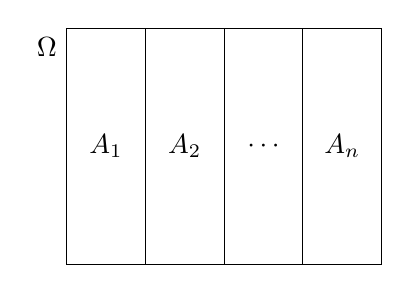
\begin{tikzpicture}
\draw (0,3) node[anchor=north east] {$\Omega$} rectangle (4,0);
\foreach \x in {1,2,3} {
	\draw (\x,0) -- (\x,3);
} 
\node at (0.5,1.5) {$A_1$};
\node at (1.5,1.5) {$A_2$};
\node at (2.5,1.5) {$\cdots$};
\node at (3.5,1.5) {$A_n$};
\end{tikzpicture}
\end{center}

Usually it is easy to get a partition of the sample space splitting a population according to some categorical variable, like for example gender, blood type, etc.
\end{frame}


%---------------------------------------------------------------------slide----
\begin{frame}
\frametitle{Total probability theorem}
If we have a partition of a sample space, we can use it to calculate the probabilities of other events in the same sample space.
\begin{theorem}[Total probability]
Given a partition $A_1,\ldots,A_n$ of a sample space $\Omega$, the probability of any other event $B$ of the same sample
space can be calculated with the formula
\[
P(B) = \sum_{i=1}^n P(A_i\cap B) = \sum_{i=1}^n P(A_i)P(B|A_i).
\]
\end{theorem}
\end{frame}


%---------------------------------------------------------------------slide----
\begin{frame}
\frametitle{Total probability theorem}
\framesubtitle{Proof}
The proof of the theorem is quite simple.
As $A_1,\ldots,A_n$ is a partition of $\Omega$, we have 
\[
B = B\cap \Omega = B\cap (A_1\cup \cdots \cup A_n) = (B\cap A_1)\cup \cdots \cup (B\cap A_n).
\]
And all the events of this union are mutually incompatible as $A_1,\ldots,A_n$ are, thus
\begin{align*}
P(B) &= P((B\cap A_1)\cup \cdots \cup (B\cap A_n)) = P(B\cap A_1)+\cdots + P(B\cap A_n) =\\
&= P(A_1)P(B|A_1)+\cdots + P(A_n)P(B|A_n) = \sum_{i=1}^n P(A_i)P(B|A_i).
\end{align*}

\begin{center}
\tikzsetnextfilename{probability/total_probability}
\mode<article>{\resizebox{0.4\textwidth}{!}{% Author: Alfredo Sánchez Alberca (asalber@ceu.es)

\begin{tikzpicture}
\def\ellipse {(2,1.5) ellipse (1.9cm and 1cm)};
\draw (0,3) node[anchor=north east] {$\Omega$} rectangle (4,0);
\foreach \x in {1,2,3} {
	\draw (\x,0) -- (\x,3);
};

\draw \ellipse;
\node at (2.5,2.2) {$B$};

\node at (0.5,0.2) {$A_1$};
\node at (1.5,0.2) {$A_2$};
\node at (2.5,0.2) {$\cdots$};
\node at (3.5,0.2) {$A_n$};


\pause
\begin{scope}
\clip (0,0) rectangle (1,3);
\draw[fill=color1!30] \ellipse;
\draw (1,0) -- (1,3);
\node[font=\scriptsize] at (0.6,1.5) {$A_1\cap B$}; 
\end{scope}
\pause
\begin{scope}
\clip (1,0) rectangle (2,3);
\draw[fill=color1!30] \ellipse;
\draw (1,0) -- (1,3);
\draw (2,0) -- (2,3);
\node[font=\scriptsize] at (1.5,1.5) {$A_2\cap B$}; 
\end{scope}
\pause
\begin{scope}
\clip (2,0) rectangle (3,3);
\draw[fill=color1!30] \ellipse;
\draw (2,0) -- (2,3);
\draw (3,0) -- (3,3);
\node at (2.5,2.2) {$B$};
\node[font=\scriptsize] at (2.5,1.5) {$\cdots$}; 
\end{scope}
\pause
\begin{scope}
\clip (3,0) rectangle (4,3);
\draw[fill=color1!30] \ellipse;
\draw (3,0) -- (3,3);
\node[font=\scriptsize] at (3.4,1.5) {$A_n\cap B$}; 
\end{scope}
\end{tikzpicture}}}
\mode<presentation>{% Author: Alfredo Sánchez Alberca (asalber@ceu.es)

\begin{tikzpicture}
\def\ellipse {(2,1.5) ellipse (1.9cm and 1cm)};
\draw (0,3) node[anchor=north east] {$\Omega$} rectangle (4,0);
\foreach \x in {1,2,3} {
	\draw (\x,0) -- (\x,3);
};

\draw \ellipse;
\node at (2.5,2.2) {$B$};

\node at (0.5,0.2) {$A_1$};
\node at (1.5,0.2) {$A_2$};
\node at (2.5,0.2) {$\cdots$};
\node at (3.5,0.2) {$A_n$};


\pause
\begin{scope}
\clip (0,0) rectangle (1,3);
\draw[fill=color1!30] \ellipse;
\draw (1,0) -- (1,3);
\node[font=\scriptsize] at (0.6,1.5) {$A_1\cap B$}; 
\end{scope}
\pause
\begin{scope}
\clip (1,0) rectangle (2,3);
\draw[fill=color1!30] \ellipse;
\draw (1,0) -- (1,3);
\draw (2,0) -- (2,3);
\node[font=\scriptsize] at (1.5,1.5) {$A_2\cap B$}; 
\end{scope}
\pause
\begin{scope}
\clip (2,0) rectangle (3,3);
\draw[fill=color1!30] \ellipse;
\draw (2,0) -- (2,3);
\draw (3,0) -- (3,3);
\node at (2.5,2.2) {$B$};
\node[font=\scriptsize] at (2.5,1.5) {$\cdots$}; 
\end{scope}
\pause
\begin{scope}
\clip (3,0) rectangle (4,3);
\draw[fill=color1!30] \ellipse;
\draw (3,0) -- (3,3);
\node[font=\scriptsize] at (3.4,1.5) {$A_n\cap B$}; 
\end{scope}
\end{tikzpicture}}
\end{center}
\end{frame}


%---------------------------------------------------------------------slide----
\begin{frame}
\frametitle{Total probability theorem}
\framesubtitle{Example of diagnosis}
A symptom $S$ can be caused by a disease $D$, but it can also be present in persons without the disease.
In a population, the rate of people with the disease is $0.2$. 
We know also that $90\%$ of persons with the disease have the symptom, while only $40\%$ of persons without the disease have it. 

\emph{What is the probability that a random person of the population has the symptom?}

To answer the question we can apply the total probability theorem using the partition $\{D,\overline D\}$:
\[
P(S) = P(D)P(S|D)+P(\overline D)P(S|\overline D) = 0.2\cdot 0.9 + 0.8\cdot 0.4 = 0.5.
\]
That is, half of the population has the symptom. 

\begin{center}
\emph{Indeed, it is a weighted mean of probabilities!}
\end{center}
\end{frame}


%---------------------------------------------------------------------slide----
\begin{frame}
\frametitle{Total probability theorem}
\framesubtitle{Example of diagnosis with a tree diagram}
The answer to the previous question is even clearer with the tree diagram of the probability space.

\begin{center}
\tikzsetnextfilename{probability/total_probability_space}
\mode<article>{\resizebox{0.6\textwidth}{!}{% Author: Alfredo Sánchez Alberca (asalber@ceu.es)

\begin{tikzpicture}[
grow'=right,
% sloped,
level 1/.style ={level distance=2cm, sibling distance=1.6cm, parent anchor=east, child anchor=west},
level 2/.style ={level distance=2cm, sibling distance=0.8cm},
level 3/.style ={level distance=1.5cm, sibling distance=0.8cm, dashed},
level 4/.style ={level distance=3cm, sibling distance=0.8cm, dashed},
prob/.style={font=\footnotesize,above}
]


\node (root) {}
	child {node {$D$}
		child {node {$S$}
			child {node[color=color2]{$(D,S)$}
				child {node[color=color2]{$0.18$} edge from parent node[prob] {$0.2\cdot 0.9$}}
			}
			edge from parent node[prob] {$0.9$}
		}
		child {node {$\bar S$}
			child {node{$(D,\bar S)$}
				child {node{$0.02$} edge from parent node[prob] {$0.2\cdot 0.1$}}
			}
			edge from parent node[prob,below] {$0.1$}
		}
		edge from parent node[prob] {$0.2$}
	}
	child {node {$\bar D$}
		child {node {$S$}
			child {node[color=color2]{$(\bar D,S)$}
				child {node[color=color2]{$0.32$} edge from parent node[prob] {$0.8\cdot 0.4$}}
			}
			edge from parent node[prob] {$0.4$}
		}
		child {node {$\bar S$}
			child {node{$(\bar D,\bar S)$}
				child {node{$0.48$} edge from parent node[prob] {$0.8\cdot 0.6$}}
			}
			edge from parent node[prob,below] {$0.6$}
		}
		edge from parent node[prob,below] {$0.8$}
	};

\begin{scope}[every node/.style={text width=2cm, align=center, anchor=center, font=\bfseries,}]
\node[above= 0.5cm of root-1-1-1-1] (labels-level) {Probability};
\node[at =(labels-level-|root-1-1-1)] {$\Omega$};
\node[at =(labels-level-|root-1-1)] {Symptom};
\node[at =(labels-level-|root-1)] {Disease};
\end{scope}
\end{tikzpicture}
}}
\mode<presentation>{\resizebox{0.8\textwidth}{!}{% Author: Alfredo Sánchez Alberca (asalber@ceu.es)

\begin{tikzpicture}[
grow'=right,
% sloped,
level 1/.style ={level distance=2cm, sibling distance=1.6cm, parent anchor=east, child anchor=west},
level 2/.style ={level distance=2cm, sibling distance=0.8cm},
level 3/.style ={level distance=1.5cm, sibling distance=0.8cm, dashed},
level 4/.style ={level distance=3cm, sibling distance=0.8cm, dashed},
prob/.style={font=\footnotesize,above}
]


\node (root) {}
	child {node {$D$}
		child {node {$S$}
			child {node[color=color2]{$(D,S)$}
				child {node[color=color2]{$0.18$} edge from parent node[prob] {$0.2\cdot 0.9$}}
			}
			edge from parent node[prob] {$0.9$}
		}
		child {node {$\bar S$}
			child {node{$(D,\bar S)$}
				child {node{$0.02$} edge from parent node[prob] {$0.2\cdot 0.1$}}
			}
			edge from parent node[prob,below] {$0.1$}
		}
		edge from parent node[prob] {$0.2$}
	}
	child {node {$\bar D$}
		child {node {$S$}
			child {node[color=color2]{$(\bar D,S)$}
				child {node[color=color2]{$0.32$} edge from parent node[prob] {$0.8\cdot 0.4$}}
			}
			edge from parent node[prob] {$0.4$}
		}
		child {node {$\bar S$}
			child {node{$(\bar D,\bar S)$}
				child {node{$0.48$} edge from parent node[prob] {$0.8\cdot 0.6$}}
			}
			edge from parent node[prob,below] {$0.6$}
		}
		edge from parent node[prob,below] {$0.8$}
	};

\begin{scope}[every node/.style={text width=2cm, align=center, anchor=center, font=\bfseries,}]
\node[above= 0.5cm of root-1-1-1-1] (labels-level) {Probability};
\node[at =(labels-level-|root-1-1-1)] {$\Omega$};
\node[at =(labels-level-|root-1-1)] {Symptom};
\node[at =(labels-level-|root-1)] {Disease};
\end{scope}
\end{tikzpicture}
}}
\end{center}

\begin{align*}
P(S) &= P(D\cap S) + P(\overline D\cap S) = P(D)P(S|D)+P(\overline D)P(S|\overline D)\\
& = 0.2\cdot 0.9+ 0.8\cdot 0.4 = 0.18 + 0.32 = 0.5.
\end{align*}
\end{frame}


\subsection{Bayes theorem}

%---------------------------------------------------------------------slide----
\begin{frame}
\frametitle{Bayes theorem}
A partition of a sample space $A_1,\cdots,A_n$ may also be interpreted as a set of feasible hypothesis for a fact $B$.

In such cases it may be helpful to calculate the posterior probability $P(A_i|B)$ of every hypothesis.

\begin{theorem}[Bayes]
Given a partition $A_1,\ldots,A_n$ of a sample space $\Omega$ and another event $B$ of the same sample space, the
conditional probability of every even $A_i$ $i=1,\ldots,n$ on $B$ can be calculated with the following formula
\[
P(A_i|B) = \frac{P(A_i\cap B)}{P(B)} = \frac{P(A_i)P(B|A_i)}{\sum_{i=1}^n P(A_i)P(B|A_i)}.
\]
\end{theorem}
\end{frame}


%---------------------------------------------------------------------slide----
\begin{frame}
\frametitle{Bayes theorem}
\framesubtitle{Example of diagnosis}
In the previous example, a more interesting question is about the diagnosis for a person with the symptom.  

In this case we can interpret $D$ and $\overline{D}$ as the two feasible hypothesis for the symptom $S$.
The prior probabilities for them are $P(D)=0.2$ and $P(\overline{D})=0.8$.
That means that if we do not have information about the symptom, the diagnosis would be that the person does not have the disease.

However, if after examining the person we observe the symptom, that information changes the uncertainty about the hypothesis, and we need calculate the posterior probabilities to diagnose, that is,
\[
P(D|S) \mbox{ and } P(\overline{D}|S)
\]
\end{frame}


%---------------------------------------------------------------------slide----
\begin{frame}
\frametitle{Bayes theorem}
\framesubtitle{Example of diagnosis}
To calculate the posterior probabilities we can use the Bayes theorem.
\begin{align*}
P(D|S) &= \frac{P(D)P(S|D)}{P(D)P(S|D)+P(\overline{D})P(S|\overline{D})} = \frac{0.2\cdot 0.9}{0.2\cdot 0.9 + 0.8\cdot 0.4} = \frac{0.18}{0.5}=0.36,\\
P(\overline{D}|S) &= \frac{P(\overline{D})P(S|\overline{D})}{P(D)P(S|D)+P(\overline{D})P(S|\overline{D})} = \frac{0.8\cdot 0.4}{0.2\cdot 0.9 + 0.8\cdot 0.4} = \frac{0.32}{0.5}=0.64.
\end{align*}

As we can see the probability of having the disease has increased. 
Nevertheless, the probability of not having the disease is still greater than the probability of having it, and for that
reason, the diagnosis is not having the disease. 

In this case it is said the the symptom $S$ is \emph{not decisive} in order to diagnose the disease.
\end{frame}


\subsection{Epidemiology}

%---------------------------------------------------------------------slide----
\begin{frame}
\frametitle{Epidemiology}
One of the branches of Medicine that makes an intensive use of probability is \highlight{Epidemilogy}, that study the distribution and causes of diseases in populations identifying risk factors for disease and targets for preventive healthcare.

In Epidemiology we are interested in how often appears a \emph{medical event} $D$ (typically a disease like flu, a risk factor like smoking or a protection factor like a vaccine) that is measured as a nominal variable with two categories (occurrence or not of the event). 

There are different measures related to the frequency of a medical event.
The most important are:
\begin{itemize}
  \item Prevalence
  \item Incidence
  \item Relative risk
  \item Odds ratio
\end{itemize}
\end{frame}


%---------------------------------------------------------------------slide----
\begin{frame}
\frametitle{Prevalence}
\begin{definition}[Prevalence]
The \emph{prevalence} of a medical event $D$ is the proportion of a particular population that is affected by a medical event.
\[
  \mbox{Prevalence}(D) = \frac{\mbox{Num people affected by $D$}}{\mbox{Population size}}
\]
\end{definition}

Often, the prevalence is estimated from a sample as the relative frequency of people affected by the event in the sample.
It is also common to express that frequency as a percentage. 

\textbf{Example}. To estimate the prevalence of flu a sample of 1000 persons has been studied and 150 of them had flu. 
Thus, the prevalence of flu is approximately 150/1000=0.15, that is, a 15\%. 

\end{frame}
  

%---------------------------------------------------------------------slide----
\begin{frame}
\frametitle{Incidence}
\highlight{Incidence} measures the likelihood of occurrence of a medical event in a population within a given period of time.
Incidence can be measured as a cumulative proportion or as a rate.

\begin{definition}[Cumulative incidence]
The \emph{cumulative incidence} of a medical event $D$ is the proportion of people that acquired the event in a period of time, that is, the number of new cases with the event in the period of time divided by the size of the population at risk.
\[
  R(D)=\frac{\mbox{Num of new cases with $D$}}{\mbox{Population at risk size}}
\]
\end{definition}

\textbf{Example}. A population initially contains $1000$ persons without flu and after two years of observation 160 of them got the flu. 
The incidence proportion of flu is 160 cases per $1000$ persons per two years, i.e. 16\% per two years.
\end{frame}
  

%---------------------------------------------------------------------slide----
\begin{frame}
\frametitle{Incidence rate or Absolute risk}
  
\begin{definition}[Incidence rate]
The \emph{incidence rate} or \emph{absolute risk} of a medical event $D$ is the number of new cases with the event divided by the size of the population at risk and by the number of units of time in a given period.
\[
  R(D)=\frac{\mbox{Num of new cases with $D$}}{\mbox{Population at risk size}\times \mbox{Num of time units}}
\]
\end{definition}

\textbf{Example}. A population initially contains $1000$ persons without flu and after two years of observation 160 of them got the flu. 
If we consider the year as the unit of time, the incidence rate of flu is 160 cases per $1000$ persons divided by two years, i.e. 80 cases per 1000 persons-year or 8\% persons per year.
\end{frame}


%---------------------------------------------------------------------slide----
\begin{frame}
\frametitle{Prevalence vs Incidence}
Prevalence must not be confused with incidence. Prevalence indicates how widespread the medical event is, and is more a measure of the burden of the event on society with no regard to time at risk or when subjects may have been exposed to a possible risk factor, whereas incidence conveys information about the risk of being affected by the event.

Prevalence can be measured in cross-sectional studies at a particular time, while in order to measure incidence we need a longitudinal study observing the individuals during a period of time.

Incidence is usually more useful than prevalence in understanding the event etiology: for example, if the incidence of a disease in a population increases, then there is a risk factor that promotes it.

When the incidence is approximately constant for the duration of the event, prevalence is approximately the product of event incidence and average event duration, so 
\begin{center}
  prevalence = incidence $\times$ duration
\end{center}
\end{frame}
  

%---------------------------------------------------------------------slide----
\begin{frame}
\frametitle{Comparing risks}
In order to determine if a factor or characteristic is associated with the medical event we need to compare the risk of the medical event in two populations, one exposed to the factor and the other not exposed.
The group of people exposed to the factor is known as the \emph{treatment group} or the \emph{experimental group} and the group of people unexposed as the \emph{control group}.

Usually the cases observed for each group are represented in a 2$\times$2 table like the one below. 

\begin{center}
  \begin{tabular}{|m{3cm}|m{3cm}<{\centering}|m{3cm}<{\centering}|}
  \cline{2-3}
  \multicolumn{1}{c|}{} & Event $D$ & No event $\overline D$\\ 
  \hline
  Treatment group\newline (exposed) & $a$ & $b$\\ 
  \hline 
  Control group\newline (unexposed) & $c$ & $d$\\ 
  \hline
  \end{tabular}
\end{center}
\end{frame}
  

%---------------------------------------------------------------------slide----
\begin{frame}
\frametitle{Attributable risk or Risk difference $RD$}
\begin{definition}[Attributable risk]
The \emph{attributable risk} or \emph{risk difference} of a medical event $D$ for people exposed to a factor is the difference between the absolute risks of the treatment group and the control group.
\[
  AR(D)=R_T(D)-R_C(D)=\frac{a}{a+b}-\frac{c}{c+d}.
\]
\end{definition}

The attributable risk is the risk of an event that is specifically due to the factor of interest.

Observe that the attributable risk can be positive, when the risk of the treatment group is greater than the risk of the control group, and negative, on the contrary.
\end{frame}


%---------------------------------------------------------------------slide----
\begin{frame}
  \frametitle{Attributable risk $RR$}
  \framesubtitle{Example of a vaccine}
  To determine the effectiveness of a vaccine against the flu, a sample of 1000 person without flu was selected at the beginning of the year.
  Half of them were vaccinated (treatment group) and the other received a placebo (control group).
  The table below summarize the results at the end of the year. 
  
  \begin{center}
    \begin{tabular}{|m{2.7cm}|m{1.5cm}<{\centering}|m{1.5cm}<{\centering}|}
    \cline{2-3}
    \multicolumn{1}{c|}{} & Flu $D$ & No flu $\overline D$\\ 
    \hline
    Treatment group\newline (vaccinated) & $20$ & $480$\\ 
    \hline 
    Control group\newline (Unvaccinated) & $80$ & $420$\\ 
    \hline
  \end{tabular}
  \end{center}
  
  The attributable risk of getting the flu for people vaccinated is
  \[
    AR(D) = \frac{20}{20+480}-\frac{80}{80+420} = -0.12.
  \]
  This means that the risk of getting flu in vaccinated people is a 12\% less than in unvaccinated. 
  \end{frame}


%---------------------------------------------------------------------slide----
\begin{frame}
\frametitle{Relative risk $RR$}
\begin{definition}[Relative risk]
The \emph{relative risk} of a medical event $D$ for people exposed to a factor is the quotient between the proportions of people that acquired the event in a period of time in the treatment and control groups.
That is, the quotient between the incidences of the treatment and the control groups.
\[
  RR(D)=\frac{\mbox{Risk in treatment group}}{\mbox{Risk in control group}}=\frac{R_T(D)}{R_C(D)}=\frac{a/(a+b)}{c/(c+d)}
\]
\end{definition}

Relative risk compares the risk of a medical event between the treatment and the control groups. 
\begin{itemize}
  \item $RR=1$ $\Rightarrow$ There is no association between the event and the exposure to the factor. 
  \item $RR<1$ $\Rightarrow$ Exposure to the factor decreases the risk of the event.
  \item $RR>1$ $\Rightarrow$ Exposure to the factor increases the risk of the event.
\end{itemize}
The further from 1, the stronger the association. 
\end{frame}


%---------------------------------------------------------------------slide----
\begin{frame}
\frametitle{Relative risk $RR$}
\framesubtitle{Example of a vaccine}
To determine the effectiveness of a vaccine against the flu, a sample of 1000 person without flu was selected at the beginning of the year.
Half of them were vaccinated (treatment group) and the other received a placebo (control group).
The table below summarize the results at the end of the year. 

\begin{center}
  \begin{tabular}{|m{2.7cm}|m{1.5cm}<{\centering}|m{1.5cm}<{\centering}|}
  \cline{2-3}
  \multicolumn{1}{c|}{} & Flu $D$ & No flu $\overline D$\\ 
  \hline
  Treatment group\newline (vaccinated) & $20$ & $480$\\ 
  \hline 
  Control group\newline (Unvaccinated) & $80$ & $420$\\ 
  \hline
\end{tabular}
\end{center}

The relative risk of getting the flu for people vaccinated is
\[
  RR(D) = \frac{20/(20+480)}{80/(80+420)} = 0.25.
\]
This means that vaccinated people were only one-fourth as likely to develop flu as were unvaccinated people, i.e. the vaccine reduce the risk of flu by 75\%.
\end{frame}


%---------------------------------------------------------------------slide----
\begin{frame}
\frametitle{Odds}
An alternative way of measuring the risk of a medical event is the \emph{odds}.

\begin{definition}[Odds]
The \emph{odds} of a medical event $D$ in a population is the quotient between the people that acquired the event and people that not in a period of time.
\[
	ODDS(D)=\frac{\mbox{Num new cases with $D$}}{\mbox{Num cases without $D$}}=\frac{P(D)}{P(\overline D)}
\]
\end{definition}

Unlike incidence, that is a proportion less than or equal to 1, the odds can be greater than 1. 
However, it is possible to convert an odds into a probability with the formula
\[
  P(D) = \frac{ODDS(D)}{ODDS(D)+1}
\]

\textbf{Example} A population initially contains $1000$ persons without flu and after a year 160 of them got the flu. 
The odds of flu is 160/840.

Observe that the incidence is 160/1000. 
\end{frame}
 

%---------------------------------------------------------------------slide----
\begin{frame}
\frametitle{Odds ratio $OR$}
\begin{definition}[Odds ratio]
The \emph{odds ratio} of a medical event $D$ for people exposed to a factor is the quotient between the odds of the event of the treatment and the control groups.
\[
  OR(D)=\frac{\mbox{Odds in treatment group}}{\mbox{Odds in control group}}=\frac{a/b}{c/d}=\frac{ad}{bc}
\]
\end{definition}

Odds ratio compares the odds of a medical event between the treatment and the control groups. 
The interpretation is similar to the relative risk. 
\begin{itemize}
  \item $OR=1$ $\Rightarrow$ There is no association between the event and the exposure to the factor. 
  \item $OR<1$ $\Rightarrow$ Exposure to the factor decreases the risk of the event.
  \item $OR>1$ $\Rightarrow$ Exposure to the factor increases the risk of the event.
\end{itemize}
The further from 1, the stronger the association. 
\end{frame}


%---------------------------------------------------------------------slide----
\begin{frame}
\frametitle{Odds ratio $OR$}
\framesubtitle{Example of a vaccine}
To determine the effectiveness of a vaccine against the flu, a sample of 1000 person without flu was selected at the beginning of the year.
Half of them were vaccinated (treatment group) and the other received a placebo (control group).
The table below summarize the results at the end of the year. 

\begin{center}
  \begin{tabular}{|m{2.7cm}|m{1.5cm}<{\centering}|m{1.5cm}<{\centering}|}
  \cline{2-3}
  \multicolumn{1}{c|}{} & Flu $D$ & No flu $\overline D$\\ 
  \hline
  Treatment group\newline (vaccinated) & $20$ & $480$\\ 
  \hline 
  Control group\newline (Unvaccinated) & $80$ & $420$\\ 
  \hline
\end{tabular}
\end{center}

The odds ratio of getting the flu for people vaccinated is
\[
  OR(D) = \frac{20/480}{80/420} = 0.21875.
\]
This means that the odds of getting the flu versus not getting the flu in vaccinated individuals is almost one fifth of that in unvaccinated, i.e. approximately for every 22 persons vaccinated with flu there will be 100 persons unvaccinated with flu. 
\end{frame}


\begin{frame}
\frametitle{Relative risk vs Odds ratio} 
Relative risk and odds ratio are two measures of association but their interpretation is slightly different.
While the relative risk expresses a comparison of risks between the treatment and control groups, the odds ratio expresses a comparison of odds, that is not the same than the risk.
Thus, an odds ratio of 2 \emph{does not} mean that the treatment group has the double of risk of acquire the medical event. 

The interpretation of the odds ratio is trickier because is counterfactual, and give us how many times is more frequent the event in the treatment group in comparison with the control group, assuming that in the control group the event is as frequent as the non-event.

The advantage of the odds ratio is that it does not depend on the prevalence or the incidence of the event, and must be used necessarily when the number of people with the medical event is selected arbitrarily in both groups, like in the case-control studies.
\end{frame}


\begin{frame}
\frametitle{Relative risk vs Odds ratio}
\framesubtitle{Example of lung cancer and smoking}
In order to determine the association between lung cancer and smoking two samples were selected (the second one with the double of non-cancer individuals) getting the following results:

\bigskip
\begin{columns}
\begin{column}{0.5\textwidth}
\textbf{Sample 1}
\begin{center}
\small
\begin{tabular}{|m{1.9cm}|m{1.2cm}<{\centering}|m{1.5cm}<{\centering}|}
\cline{2-3}
\multicolumn{1}{c|}{} & Cancer & No cancer\\ 
\hline
Smokers & $60$ & $80$\\ 
\hline 
Non-smokers & $40$ & $320$\\ 
\hline
\end{tabular}
\end{center}

\begin{align*}
RR(D) &= \frac{60/(60+80)}{40/(40+320)} = 3.86.\\
OR(D) &= \frac{60/80}{40/320} = 6. 
\end{align*}
\end{column}
\begin{column}{0.5\textwidth}
\textbf{Sample 2}
\begin{center}
\small
\begin{tabular}{|m{1.9cm}|m{1.2cm}<{\centering}|m{1.5cm}<{\centering}|}
\cline{2-3}
\multicolumn{1}{c|}{} & Cancer & No cancer\\ 
\hline
Smokers & $60$ & $160$\\ 
\hline 
Non-smokers & $40$ & $640$\\ 
\hline
\end{tabular}
\end{center}

\begin{align*}
RR(D) &= \frac{60/(60+160)}{40/(40+640)} = 4.64.\\
OR(D) &= \frac{60/160}{40/640} = 6. 
\end{align*}
\end{column}
\end{columns}
Thus, when we change the incidence or the prevalence of the event (lung cancer) the relative risk changes, while the odds ratio not. 
\end{frame}


\begin{frame}
\frametitle{Relative risk vs Odds ratio} 
The relation between the relative risk and the odds ratio is given by the following formula

\[
  RR = \frac{OR}{1-R_C+R_C*OR}=OR*\frac{1-R_T}{1-R_C},
\]

where $R_C$ and $R_T$ are the prevalence or the incidence in control and treatment groups respectively.

The odds ratio always overestimate the relative risk when it is greater than 1 and underestimate it when it is less than 1. 
However, with rare medical events (with very small prevalence or incidence) the relative risk and the odds ratio are almost the same. 
\end{frame}


\begin{frame}
\frametitle{Relative risk vs Odds ratio} 
\begin{center}
\tikzsetnextfilename{probability/odds_ratio_vs_relative_risk}
\mode<article>{\resizebox{0.6\textwidth}{!}{% Created by tikzDevice version 0.10.1.2 on 2018-02-15 11:51:08
% !TEX encoding = UTF-8 Unicode
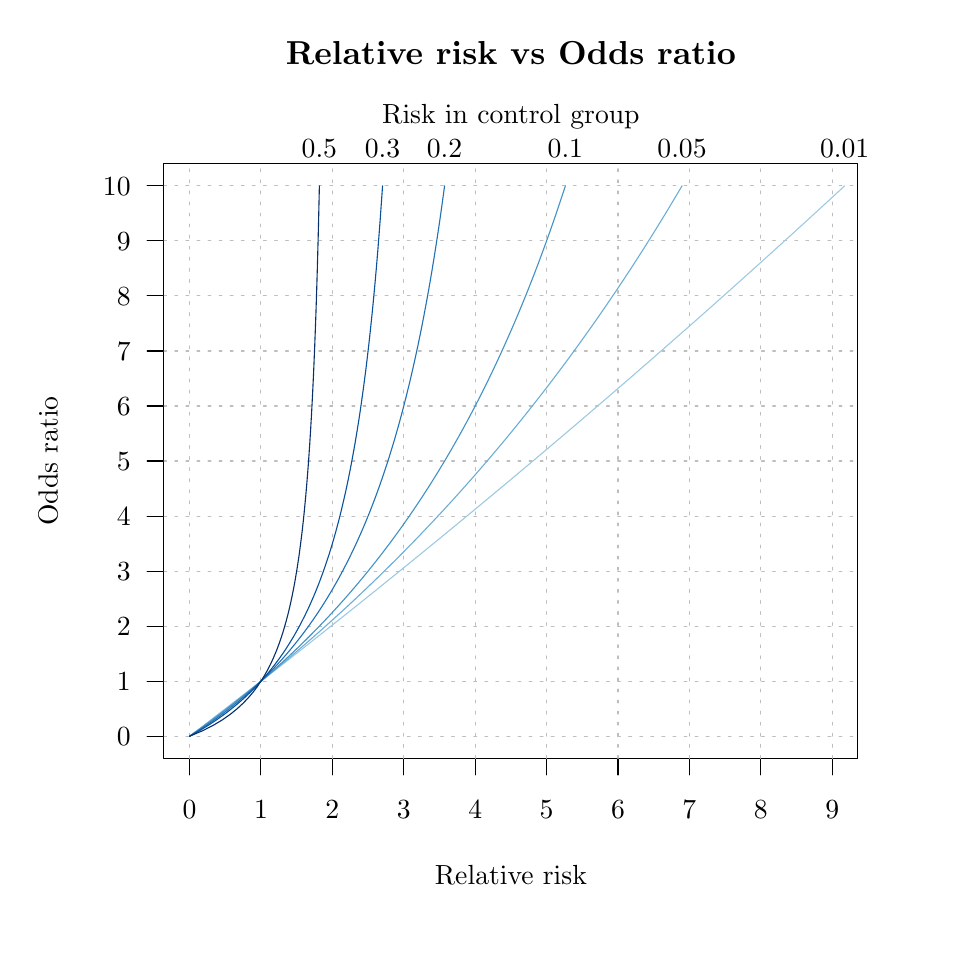
\begin{tikzpicture}[x=1pt,y=1pt]
\definecolor{fillColor}{RGB}{255,255,255}
\path[use as bounding box,fill=fillColor,fill opacity=0.00] (0,0) rectangle (325.21,325.21);
\begin{scope}
\path[clip] (  0.00,  0.00) rectangle (325.21,325.21);
\definecolor{drawColor}{RGB}{0,0,0}

\path[draw=drawColor,line width= 0.4pt,line join=round,line cap=round] ( 49.20, 61.20) --
	(300.01, 61.20) --
	(300.01,276.01) --
	( 49.20,276.01) --
	( 49.20, 61.20);
\end{scope}
\begin{scope}
\path[clip] (  0.00,  0.00) rectangle (325.21,325.21);
\definecolor{drawColor}{RGB}{0,0,0}

\node[text=drawColor,anchor=base,inner sep=0pt, outer sep=0pt, scale=  1.00] at (174.61, 15.60) {Relative risk};

\node[text=drawColor,rotate= 90.00,anchor=base,inner sep=0pt, outer sep=0pt, scale=  1.00] at ( 10.80,168.61) {Odds ratio};
\end{scope}
\begin{scope}
\path[clip] (  0.00,  0.00) rectangle (325.21,325.21);
\definecolor{drawColor}{RGB}{0,0,0}

\path[draw=drawColor,line width= 0.4pt,line join=round,line cap=round] ( 49.20, 69.16) -- ( 49.20,268.06);

\path[draw=drawColor,line width= 0.4pt,line join=round,line cap=round] ( 49.20, 69.16) -- ( 43.20, 69.16);

\path[draw=drawColor,line width= 0.4pt,line join=round,line cap=round] ( 49.20, 89.05) -- ( 43.20, 89.05);

\path[draw=drawColor,line width= 0.4pt,line join=round,line cap=round] ( 49.20,108.94) -- ( 43.20,108.94);

\path[draw=drawColor,line width= 0.4pt,line join=round,line cap=round] ( 49.20,128.83) -- ( 43.20,128.83);

\path[draw=drawColor,line width= 0.4pt,line join=round,line cap=round] ( 49.20,148.72) -- ( 43.20,148.72);

\path[draw=drawColor,line width= 0.4pt,line join=round,line cap=round] ( 49.20,168.61) -- ( 43.20,168.61);

\path[draw=drawColor,line width= 0.4pt,line join=round,line cap=round] ( 49.20,188.50) -- ( 43.20,188.50);

\path[draw=drawColor,line width= 0.4pt,line join=round,line cap=round] ( 49.20,208.39) -- ( 43.20,208.39);

\path[draw=drawColor,line width= 0.4pt,line join=round,line cap=round] ( 49.20,228.28) -- ( 43.20,228.28);

\path[draw=drawColor,line width= 0.4pt,line join=round,line cap=round] ( 49.20,248.17) -- ( 43.20,248.17);

\path[draw=drawColor,line width= 0.4pt,line join=round,line cap=round] ( 49.20,268.06) -- ( 43.20,268.06);

\node[text=drawColor,anchor=base east,inner sep=0pt, outer sep=0pt, scale=  1.00] at ( 37.20, 65.71) {0};

\node[text=drawColor,anchor=base east,inner sep=0pt, outer sep=0pt, scale=  1.00] at ( 37.20, 85.60) {1};

\node[text=drawColor,anchor=base east,inner sep=0pt, outer sep=0pt, scale=  1.00] at ( 37.20,105.49) {2};

\node[text=drawColor,anchor=base east,inner sep=0pt, outer sep=0pt, scale=  1.00] at ( 37.20,125.38) {3};

\node[text=drawColor,anchor=base east,inner sep=0pt, outer sep=0pt, scale=  1.00] at ( 37.20,145.27) {4};

\node[text=drawColor,anchor=base east,inner sep=0pt, outer sep=0pt, scale=  1.00] at ( 37.20,165.16) {5};

\node[text=drawColor,anchor=base east,inner sep=0pt, outer sep=0pt, scale=  1.00] at ( 37.20,185.05) {6};

\node[text=drawColor,anchor=base east,inner sep=0pt, outer sep=0pt, scale=  1.00] at ( 37.20,204.94) {7};

\node[text=drawColor,anchor=base east,inner sep=0pt, outer sep=0pt, scale=  1.00] at ( 37.20,224.83) {8};

\node[text=drawColor,anchor=base east,inner sep=0pt, outer sep=0pt, scale=  1.00] at ( 37.20,244.73) {9};

\node[text=drawColor,anchor=base east,inner sep=0pt, outer sep=0pt, scale=  1.00] at ( 37.20,264.62) {10};

\path[draw=drawColor,line width= 0.4pt,line join=round,line cap=round] ( 58.49, 61.20) -- (290.73, 61.20);

\path[draw=drawColor,line width= 0.4pt,line join=round,line cap=round] ( 58.49, 61.20) -- ( 58.49, 55.20);

\path[draw=drawColor,line width= 0.4pt,line join=round,line cap=round] ( 84.29, 61.20) -- ( 84.29, 55.20);

\path[draw=drawColor,line width= 0.4pt,line join=round,line cap=round] (110.10, 61.20) -- (110.10, 55.20);

\path[draw=drawColor,line width= 0.4pt,line join=round,line cap=round] (135.90, 61.20) -- (135.90, 55.20);

\path[draw=drawColor,line width= 0.4pt,line join=round,line cap=round] (161.71, 61.20) -- (161.71, 55.20);

\path[draw=drawColor,line width= 0.4pt,line join=round,line cap=round] (187.51, 61.20) -- (187.51, 55.20);

\path[draw=drawColor,line width= 0.4pt,line join=round,line cap=round] (213.31, 61.20) -- (213.31, 55.20);

\path[draw=drawColor,line width= 0.4pt,line join=round,line cap=round] (239.12, 61.20) -- (239.12, 55.20);

\path[draw=drawColor,line width= 0.4pt,line join=round,line cap=round] (264.92, 61.20) -- (264.92, 55.20);

\path[draw=drawColor,line width= 0.4pt,line join=round,line cap=round] (290.73, 61.20) -- (290.73, 55.20);

\node[text=drawColor,anchor=base,inner sep=0pt, outer sep=0pt, scale=  1.00] at ( 58.49, 39.60) {0};

\node[text=drawColor,anchor=base,inner sep=0pt, outer sep=0pt, scale=  1.00] at ( 84.29, 39.60) {1};

\node[text=drawColor,anchor=base,inner sep=0pt, outer sep=0pt, scale=  1.00] at (110.10, 39.60) {2};

\node[text=drawColor,anchor=base,inner sep=0pt, outer sep=0pt, scale=  1.00] at (135.90, 39.60) {3};

\node[text=drawColor,anchor=base,inner sep=0pt, outer sep=0pt, scale=  1.00] at (161.71, 39.60) {4};

\node[text=drawColor,anchor=base,inner sep=0pt, outer sep=0pt, scale=  1.00] at (187.51, 39.60) {5};

\node[text=drawColor,anchor=base,inner sep=0pt, outer sep=0pt, scale=  1.00] at (213.31, 39.60) {6};

\node[text=drawColor,anchor=base,inner sep=0pt, outer sep=0pt, scale=  1.00] at (239.12, 39.60) {7};

\node[text=drawColor,anchor=base,inner sep=0pt, outer sep=0pt, scale=  1.00] at (264.92, 39.60) {8};

\node[text=drawColor,anchor=base,inner sep=0pt, outer sep=0pt, scale=  1.00] at (290.73, 39.60) {9};
\end{scope}
\begin{scope}
\path[clip] ( 49.20, 61.20) rectangle (300.01,276.01);
\definecolor{drawColor}{RGB}{190,190,190}

\path[draw=drawColor,line width= 0.4pt,dash pattern=on 1pt off 3pt ,line join=round,line cap=round] ( 49.20, 69.16) -- (300.01, 69.16);

\path[draw=drawColor,line width= 0.4pt,dash pattern=on 1pt off 3pt ,line join=round,line cap=round] ( 49.20, 89.05) -- (300.01, 89.05);

\path[draw=drawColor,line width= 0.4pt,dash pattern=on 1pt off 3pt ,line join=round,line cap=round] ( 49.20,108.94) -- (300.01,108.94);

\path[draw=drawColor,line width= 0.4pt,dash pattern=on 1pt off 3pt ,line join=round,line cap=round] ( 49.20,128.83) -- (300.01,128.83);

\path[draw=drawColor,line width= 0.4pt,dash pattern=on 1pt off 3pt ,line join=round,line cap=round] ( 49.20,148.72) -- (300.01,148.72);

\path[draw=drawColor,line width= 0.4pt,dash pattern=on 1pt off 3pt ,line join=round,line cap=round] ( 49.20,168.61) -- (300.01,168.61);

\path[draw=drawColor,line width= 0.4pt,dash pattern=on 1pt off 3pt ,line join=round,line cap=round] ( 49.20,188.50) -- (300.01,188.50);

\path[draw=drawColor,line width= 0.4pt,dash pattern=on 1pt off 3pt ,line join=round,line cap=round] ( 49.20,208.39) -- (300.01,208.39);

\path[draw=drawColor,line width= 0.4pt,dash pattern=on 1pt off 3pt ,line join=round,line cap=round] ( 49.20,228.28) -- (300.01,228.28);

\path[draw=drawColor,line width= 0.4pt,dash pattern=on 1pt off 3pt ,line join=round,line cap=round] ( 49.20,248.17) -- (300.01,248.17);

\path[draw=drawColor,line width= 0.4pt,dash pattern=on 1pt off 3pt ,line join=round,line cap=round] ( 49.20,268.06) -- (300.01,268.06);

\path[draw=drawColor,line width= 0.4pt,dash pattern=on 1pt off 3pt ,line join=round,line cap=round] ( 58.49, 61.20) -- ( 58.49,276.01);

\path[draw=drawColor,line width= 0.4pt,dash pattern=on 1pt off 3pt ,line join=round,line cap=round] ( 84.29, 61.20) -- ( 84.29,276.01);

\path[draw=drawColor,line width= 0.4pt,dash pattern=on 1pt off 3pt ,line join=round,line cap=round] (110.10, 61.20) -- (110.10,276.01);

\path[draw=drawColor,line width= 0.4pt,dash pattern=on 1pt off 3pt ,line join=round,line cap=round] (135.90, 61.20) -- (135.90,276.01);

\path[draw=drawColor,line width= 0.4pt,dash pattern=on 1pt off 3pt ,line join=round,line cap=round] (161.71, 61.20) -- (161.71,276.01);

\path[draw=drawColor,line width= 0.4pt,dash pattern=on 1pt off 3pt ,line join=round,line cap=round] (187.51, 61.20) -- (187.51,276.01);

\path[draw=drawColor,line width= 0.4pt,dash pattern=on 1pt off 3pt ,line join=round,line cap=round] (213.31, 61.20) -- (213.31,276.01);

\path[draw=drawColor,line width= 0.4pt,dash pattern=on 1pt off 3pt ,line join=round,line cap=round] (239.12, 61.20) -- (239.12,276.01);

\path[draw=drawColor,line width= 0.4pt,dash pattern=on 1pt off 3pt ,line join=round,line cap=round] (264.92, 61.20) -- (264.92,276.01);

\path[draw=drawColor,line width= 0.4pt,dash pattern=on 1pt off 3pt ,line join=round,line cap=round] (290.73, 61.20) -- (290.73,276.01);
\end{scope}
\begin{scope}
\path[clip] (  0.00,  0.00) rectangle (325.21,325.21);
\definecolor{drawColor}{RGB}{0,0,0}

\node[text=drawColor,anchor=base,inner sep=0pt, outer sep=0pt, scale=  1.20] at (174.61,312.01) {\bfseries Relative risk vs Odds ratio};
\end{scope}
\begin{scope}
\path[clip] ( 49.20, 61.20) rectangle (300.01,276.01);
\definecolor{drawColor}{RGB}{158,202,225}

\path[draw=drawColor,line width= 0.4pt,line join=round,line cap=round] ( 58.49, 69.16) --
	( 61.09, 71.15) --
	( 63.69, 73.13) --
	( 66.29, 75.12) --
	( 68.87, 77.11) --
	( 71.46, 79.10) --
	( 74.03, 81.09) --
	( 76.61, 83.08) --
	( 79.17, 85.07) --
	( 81.74, 87.06) --
	( 84.29, 89.05) --
	( 86.85, 91.04) --
	( 89.39, 93.02) --
	( 91.93, 95.01) --
	( 94.47, 97.00) --
	( 97.00, 98.99) --
	( 99.53,100.98) --
	(102.05,102.97) --
	(104.57,104.96) --
	(107.08,106.95) --
	(109.59,108.94) --
	(112.09,110.93) --
	(114.59,112.91) --
	(117.08,114.90) --
	(119.56,116.89) --
	(122.05,118.88) --
	(124.52,120.87) --
	(127.00,122.86) --
	(129.46,124.85) --
	(131.93,126.84) --
	(134.38,128.83) --
	(136.84,130.82) --
	(139.28,132.80) --
	(141.73,134.79) --
	(144.17,136.78) --
	(146.60,138.77) --
	(149.03,140.76) --
	(151.45,142.75) --
	(153.87,144.74) --
	(156.29,146.73) --
	(158.70,148.72) --
	(161.10,150.71) --
	(163.51,152.70) --
	(165.90,154.68) --
	(168.29,156.67) --
	(170.68,158.66) --
	(173.06,160.65) --
	(175.44,162.64) --
	(177.81,164.63) --
	(180.18,166.62) --
	(182.55,168.61) --
	(184.91,170.60) --
	(187.26,172.59) --
	(189.61,174.57) --
	(191.96,176.56) --
	(194.30,178.55) --
	(196.64,180.54) --
	(198.97,182.53) --
	(201.30,184.52) --
	(203.62,186.51) --
	(205.94,188.50) --
	(208.26,190.49) --
	(210.57,192.48) --
	(212.87,194.46) --
	(215.17,196.45) --
	(217.47,198.44) --
	(219.76,200.43) --
	(222.05,202.42) --
	(224.34,204.41) --
	(226.62,206.40) --
	(228.89,208.39) --
	(231.16,210.38) --
	(233.43,212.37) --
	(235.69,214.36) --
	(237.95,216.34) --
	(240.21,218.33) --
	(242.46,220.32) --
	(244.70,222.31) --
	(246.95,224.30) --
	(249.18,226.29) --
	(251.42,228.28) --
	(253.65,230.27) --
	(255.87,232.26) --
	(258.09,234.25) --
	(260.31,236.23) --
	(262.52,238.22) --
	(264.73,240.21) --
	(266.93,242.20) --
	(269.13,244.19) --
	(271.33,246.18) --
	(273.52,248.17) --
	(275.71,250.16) --
	(277.90,252.15) --
	(280.08,254.14) --
	(282.25,256.12) --
	(284.42,258.11) --
	(286.59,260.10) --
	(288.76,262.09) --
	(290.92,264.08) --
	(293.07,266.07) --
	(295.22,268.06);
\end{scope}
\begin{scope}
\path[clip] (  0.00,  0.00) rectangle (325.21,325.21);
\definecolor{drawColor}{RGB}{0,0,0}

\node[text=drawColor,anchor=base,inner sep=0pt, outer sep=0pt, scale=  1.00] at (295.22,278.42) {0.01};
\end{scope}
\begin{scope}
\path[clip] ( 49.20, 61.20) rectangle (300.01,276.01);
\definecolor{drawColor}{RGB}{107,174,214}

\path[draw=drawColor,line width= 0.4pt,line join=round,line cap=round] ( 58.49, 69.16) --
	( 61.19, 71.15) --
	( 63.87, 73.13) --
	( 66.51, 75.12) --
	( 69.13, 77.11) --
	( 71.72, 79.10) --
	( 74.29, 81.09) --
	( 76.83, 83.08) --
	( 79.34, 85.07) --
	( 81.83, 87.06) --
	( 84.29, 89.05) --
	( 86.73, 91.04) --
	( 89.15, 93.02) --
	( 91.54, 95.01) --
	( 93.91, 97.00) --
	( 96.25, 98.99) --
	( 98.57,100.98) --
	(100.87,102.97) --
	(103.15,104.96) --
	(105.41,106.95) --
	(107.64,108.94) --
	(109.85,110.93) --
	(112.04,112.91) --
	(114.22,114.90) --
	(116.37,116.89) --
	(118.50,118.88) --
	(120.61,120.87) --
	(122.70,122.86) --
	(124.77,124.85) --
	(126.83,126.84) --
	(128.86,128.83) --
	(130.88,130.82) --
	(132.88,132.80) --
	(134.86,134.79) --
	(136.82,136.78) --
	(138.77,138.77) --
	(140.70,140.76) --
	(142.61,142.75) --
	(144.50,144.74) --
	(146.38,146.73) --
	(148.24,148.72) --
	(150.09,150.71) --
	(151.92,152.70) --
	(153.73,154.68) --
	(155.53,156.67) --
	(157.31,158.66) --
	(159.08,160.65) --
	(160.83,162.64) --
	(162.57,164.63) --
	(164.30,166.62) --
	(166.01,168.61) --
	(167.70,170.60) --
	(169.38,172.59) --
	(171.05,174.57) --
	(172.70,176.56) --
	(174.34,178.55) --
	(175.97,180.54) --
	(177.58,182.53) --
	(179.19,184.52) --
	(180.77,186.51) --
	(182.35,188.50) --
	(183.91,190.49) --
	(185.46,192.48) --
	(187.00,194.46) --
	(188.53,196.45) --
	(190.04,198.44) --
	(191.54,200.43) --
	(193.03,202.42) --
	(194.51,204.41) --
	(195.98,206.40) --
	(197.43,208.39) --
	(198.88,210.38) --
	(200.31,212.37) --
	(201.74,214.36) --
	(203.15,216.34) --
	(204.55,218.33) --
	(205.94,220.32) --
	(207.32,222.31) --
	(208.69,224.30) --
	(210.05,226.29) --
	(211.40,228.28) --
	(212.74,230.27) --
	(214.07,232.26) --
	(215.39,234.25) --
	(216.70,236.23) --
	(218.01,238.22) --
	(219.30,240.21) --
	(220.58,242.20) --
	(221.85,244.19) --
	(223.12,246.18) --
	(224.37,248.17) --
	(225.62,250.16) --
	(226.86,252.15) --
	(228.08,254.14) --
	(229.30,256.12) --
	(230.52,258.11) --
	(231.72,260.10) --
	(232.91,262.09) --
	(234.10,264.08) --
	(235.28,266.07) --
	(236.45,268.06);
\end{scope}
\begin{scope}
\path[clip] (  0.00,  0.00) rectangle (325.21,325.21);
\definecolor{drawColor}{RGB}{0,0,0}

\node[text=drawColor,anchor=base,inner sep=0pt, outer sep=0pt, scale=  1.00] at (236.45,278.42) {0.05};
\end{scope}
\begin{scope}
\path[clip] ( 49.20, 61.20) rectangle (300.01,276.01);
\definecolor{drawColor}{RGB}{66,146,198}

\path[draw=drawColor,line width= 0.4pt,line join=round,line cap=round] ( 58.49, 69.16) --
	( 61.33, 71.15) --
	( 64.10, 73.13) --
	( 66.81, 75.12) --
	( 69.47, 77.11) --
	( 72.07, 79.10) --
	( 74.62, 81.09) --
	( 77.11, 83.08) --
	( 79.55, 85.07) --
	( 81.95, 87.06) --
	( 84.29, 89.05) --
	( 86.59, 91.04) --
	( 88.85, 93.02) --
	( 91.06, 95.01) --
	( 93.23, 97.00) --
	( 95.35, 98.99) --
	( 97.44,100.98) --
	( 99.49,102.97) --
	(101.50,104.96) --
	(103.47,106.95) --
	(105.41,108.94) --
	(107.31,110.93) --
	(109.18,112.91) --
	(111.01,114.90) --
	(112.81,116.89) --
	(114.59,118.88) --
	(116.33,120.87) --
	(118.04,122.86) --
	(119.72,124.85) --
	(121.37,126.84) --
	(123.00,128.83) --
	(124.60,130.82) --
	(126.17,132.80) --
	(127.72,134.79) --
	(129.24,136.78) --
	(130.74,138.77) --
	(132.22,140.76) --
	(133.67,142.75) --
	(135.10,144.74) --
	(136.50,146.73) --
	(137.89,148.72) --
	(139.25,150.71) --
	(140.59,152.70) --
	(141.92,154.68) --
	(143.22,156.67) --
	(144.50,158.66) --
	(145.77,160.65) --
	(147.01,162.64) --
	(148.24,164.63) --
	(149.45,166.62) --
	(150.65,168.61) --
	(151.82,170.60) --
	(152.98,172.59) --
	(154.13,174.57) --
	(155.25,176.56) --
	(156.37,178.55) --
	(157.46,180.54) --
	(158.55,182.53) --
	(159.61,184.52) --
	(160.67,186.51) --
	(161.71,188.50) --
	(162.73,190.49) --
	(163.74,192.48) --
	(164.74,194.46) --
	(165.73,196.45) --
	(166.70,198.44) --
	(167.66,200.43) --
	(168.61,202.42) --
	(169.54,204.41) --
	(170.47,206.40) --
	(171.38,208.39) --
	(172.28,210.38) --
	(173.17,212.37) --
	(174.05,214.36) --
	(174.92,216.34) --
	(175.78,218.33) --
	(176.63,220.32) --
	(177.47,222.31) --
	(178.29,224.30) --
	(179.11,226.29) --
	(179.92,228.28) --
	(180.72,230.27) --
	(181.51,232.26) --
	(182.29,234.25) --
	(183.06,236.23) --
	(183.82,238.22) --
	(184.58,240.21) --
	(185.32,242.20) --
	(186.06,244.19) --
	(186.79,246.18) --
	(187.51,248.17) --
	(188.22,250.16) --
	(188.93,252.15) --
	(189.62,254.14) --
	(190.31,256.12) --
	(191.00,258.11) --
	(191.67,260.10) --
	(192.34,262.09) --
	(193.00,264.08) --
	(193.65,266.07) --
	(194.30,268.06);
\end{scope}
\begin{scope}
\path[clip] (  0.00,  0.00) rectangle (325.21,325.21);
\definecolor{drawColor}{RGB}{0,0,0}

\node[text=drawColor,anchor=base,inner sep=0pt, outer sep=0pt, scale=  1.00] at (194.30,278.42) {0.1};
\end{scope}
\begin{scope}
\path[clip] ( 49.20, 61.20) rectangle (300.01,276.01);
\definecolor{drawColor}{RGB}{33,113,181}

\path[draw=drawColor,line width= 0.4pt,line join=round,line cap=round] ( 58.49, 69.16) --
	( 61.64, 71.15) --
	( 64.63, 73.13) --
	( 67.49, 75.12) --
	( 70.22, 77.11) --
	( 72.83, 79.10) --
	( 75.32, 81.09) --
	( 77.71, 83.08) --
	( 79.99, 85.07) --
	( 82.19, 87.06) --
	( 84.29, 89.05) --
	( 86.32, 91.04) --
	( 88.26, 93.02) --
	( 90.14, 95.01) --
	( 91.94, 97.00) --
	( 93.68, 98.99) --
	( 95.35,100.98) --
	( 96.97,102.97) --
	( 98.53,104.96) --
	(100.04,106.95) --
	(101.50,108.94) --
	(102.91,110.93) --
	(104.27,112.91) --
	(105.59,114.90) --
	(106.87,116.89) --
	(108.11,118.88) --
	(109.32,120.87) --
	(110.48,122.86) --
	(111.62,124.85) --
	(112.72,126.84) --
	(113.78,128.83) --
	(114.82,130.82) --
	(115.83,132.80) --
	(116.81,134.79) --
	(117.77,136.78) --
	(118.70,138.77) --
	(119.60,140.76) --
	(120.49,142.75) --
	(121.35,144.74) --
	(122.18,146.73) --
	(123.00,148.72) --
	(123.80,150.71) --
	(124.57,152.70) --
	(125.33,154.68) --
	(126.07,156.67) --
	(126.79,158.66) --
	(127.50,160.65) --
	(128.19,162.64) --
	(128.86,164.63) --
	(129.52,166.62) --
	(130.17,168.61) --
	(130.80,170.60) --
	(131.41,172.59) --
	(132.02,174.57) --
	(132.61,176.56) --
	(133.19,178.55) --
	(133.75,180.54) --
	(134.31,182.53) --
	(134.85,184.52) --
	(135.38,186.51) --
	(135.90,188.50) --
	(136.41,190.49) --
	(136.91,192.48) --
	(137.40,194.46) --
	(137.89,196.45) --
	(138.36,198.44) --
	(138.82,200.43) --
	(139.28,202.42) --
	(139.72,204.41) --
	(140.16,206.40) --
	(140.59,208.39) --
	(141.02,210.38) --
	(141.43,212.37) --
	(141.84,214.36) --
	(142.24,216.34) --
	(142.63,218.33) --
	(143.02,220.32) --
	(143.40,222.31) --
	(143.77,224.30) --
	(144.14,226.29) --
	(144.50,228.28) --
	(144.86,230.27) --
	(145.21,232.26) --
	(145.55,234.25) --
	(145.89,236.23) --
	(146.22,238.22) --
	(146.55,240.21) --
	(146.87,242.20) --
	(147.19,244.19) --
	(147.50,246.18) --
	(147.81,248.17) --
	(148.11,250.16) --
	(148.41,252.15) --
	(148.71,254.14) --
	(149.00,256.12) --
	(149.28,258.11) --
	(149.56,260.10) --
	(149.84,262.09) --
	(150.11,264.08) --
	(150.38,266.07) --
	(150.65,268.06);
\end{scope}
\begin{scope}
\path[clip] (  0.00,  0.00) rectangle (325.21,325.21);
\definecolor{drawColor}{RGB}{0,0,0}

\node[text=drawColor,anchor=base,inner sep=0pt, outer sep=0pt, scale=  1.00] at (150.65,278.42) {0.2};
\end{scope}
\begin{scope}
\path[clip] ( 49.20, 61.20) rectangle (300.01,276.01);
\definecolor{drawColor}{RGB}{8,81,156}

\path[draw=drawColor,line width= 0.4pt,line join=round,line cap=round] ( 58.49, 69.16) --
	( 62.02, 71.15) --
	( 65.28, 73.13) --
	( 68.29, 75.12) --
	( 71.08, 77.11) --
	( 73.67, 79.10) --
	( 76.08, 81.09) --
	( 78.34, 83.08) --
	( 80.45, 85.07) --
	( 82.43, 87.06) --
	( 84.29, 89.05) --
	( 86.05, 91.04) --
	( 87.70, 93.02) --
	( 89.26, 95.01) --
	( 90.74, 97.00) --
	( 92.15, 98.99) --
	( 93.48,100.98) --
	( 94.74,102.97) --
	( 95.95,104.96) --
	( 97.09,106.95) --
	( 98.19,108.94) --
	( 99.23,110.93) --
	(100.23,112.91) --
	(101.19,114.90) --
	(102.10,116.89) --
	(102.98,118.88) --
	(103.82,120.87) --
	(104.63,122.86) --
	(105.41,124.85) --
	(106.15,126.84) --
	(106.87,128.83) --
	(107.56,130.82) --
	(108.23,132.80) --
	(108.88,134.79) --
	(109.50,136.78) --
	(110.10,138.77) --
	(110.68,140.76) --
	(111.24,142.75) --
	(111.78,144.74) --
	(112.31,146.73) --
	(112.81,148.72) --
	(113.31,150.71) --
	(113.78,152.70) --
	(114.25,154.68) --
	(114.70,156.67) --
	(115.13,158.66) --
	(115.56,160.65) --
	(115.97,162.64) --
	(116.37,164.63) --
	(116.76,166.62) --
	(117.13,168.61) --
	(117.50,170.60) --
	(117.86,172.59) --
	(118.21,174.57) --
	(118.55,176.56) --
	(118.88,178.55) --
	(119.20,180.54) --
	(119.52,182.53) --
	(119.83,184.52) --
	(120.13,186.51) --
	(120.42,188.50) --
	(120.70,190.49) --
	(120.98,192.48) --
	(121.26,194.46) --
	(121.52,196.45) --
	(121.78,198.44) --
	(122.04,200.43) --
	(122.29,202.42) --
	(122.53,204.41) --
	(122.77,206.40) --
	(123.00,208.39) --
	(123.23,210.38) --
	(123.45,212.37) --
	(123.67,214.36) --
	(123.88,216.34) --
	(124.09,218.33) --
	(124.30,220.32) --
	(124.50,222.31) --
	(124.70,224.30) --
	(124.89,226.29) --
	(125.08,228.28) --
	(125.27,230.27) --
	(125.45,232.26) --
	(125.63,234.25) --
	(125.80,236.23) --
	(125.98,238.22) --
	(126.15,240.21) --
	(126.31,242.20) --
	(126.48,244.19) --
	(126.64,246.18) --
	(126.79,248.17) --
	(126.95,250.16) --
	(127.10,252.15) --
	(127.25,254.14) --
	(127.40,256.12) --
	(127.54,258.11) --
	(127.68,260.10) --
	(127.82,262.09) --
	(127.96,264.08) --
	(128.10,266.07) --
	(128.23,268.06);
\end{scope}
\begin{scope}
\path[clip] (  0.00,  0.00) rectangle (325.21,325.21);
\definecolor{drawColor}{RGB}{0,0,0}

\node[text=drawColor,anchor=base,inner sep=0pt, outer sep=0pt, scale=  1.00] at (128.23,278.42) {0.3};
\end{scope}
\begin{scope}
\path[clip] ( 49.20, 61.20) rectangle (300.01,276.01);
\definecolor{drawColor}{RGB}{8,48,107}

\path[draw=drawColor,line width= 0.4pt,line join=round,line cap=round] ( 58.49, 69.16) --
	( 63.18, 71.15) --
	( 67.09, 73.13) --
	( 70.40, 75.12) --
	( 73.23, 77.11) --
	( 75.69, 79.10) --
	( 77.84, 81.09) --
	( 79.74, 83.08) --
	( 81.43, 85.07) --
	( 82.94, 87.06) --
	( 84.29, 89.05) --
	( 85.52, 91.04) --
	( 86.64, 93.02) --
	( 87.66, 95.01) --
	( 88.59, 97.00) --
	( 89.45, 98.99) --
	( 90.25,100.98) --
	( 90.98,102.97) --
	( 91.67,104.96) --
	( 92.30,106.95) --
	( 92.89,108.94) --
	( 93.45,110.93) --
	( 93.97,112.91) --
	( 94.46,114.90) --
	( 94.92,116.89) --
	( 95.35,118.88) --
	( 95.76,120.87) --
	( 96.15,122.86) --
	( 96.52,124.85) --
	( 96.86,126.84) --
	( 97.20,128.83) --
	( 97.51,130.82) --
	( 97.81,132.80) --
	( 98.10,134.79) --
	( 98.37,136.78) --
	( 98.63,138.77) --
	( 98.88,140.76) --
	( 99.12,142.75) --
	( 99.35,144.74) --
	( 99.57,146.73) --
	( 99.78,148.72) --
	( 99.98,150.71) --
	(100.17,152.70) --
	(100.36,154.68) --
	(100.54,156.67) --
	(100.71,158.66) --
	(100.88,160.65) --
	(101.04,162.64) --
	(101.20,164.63) --
	(101.35,166.62) --
	(101.50,168.61) --
	(101.64,170.60) --
	(101.77,172.59) --
	(101.91,174.57) --
	(102.03,176.56) --
	(102.16,178.55) --
	(102.28,180.54) --
	(102.39,182.53) --
	(102.51,184.52) --
	(102.62,186.51) --
	(102.72,188.50) --
	(102.83,190.49) --
	(102.93,192.48) --
	(103.03,194.46) --
	(103.12,196.45) --
	(103.22,198.44) --
	(103.31,200.43) --
	(103.40,202.42) --
	(103.48,204.41) --
	(103.56,206.40) --
	(103.65,208.39) --
	(103.73,210.38) --
	(103.80,212.37) --
	(103.88,214.36) --
	(103.95,216.34) --
	(104.03,218.33) --
	(104.10,220.32) --
	(104.17,222.31) --
	(104.23,224.30) --
	(104.30,226.29) --
	(104.36,228.28) --
	(104.43,230.27) --
	(104.49,232.26) --
	(104.55,234.25) --
	(104.61,236.23) --
	(104.67,238.22) --
	(104.72,240.21) --
	(104.78,242.20) --
	(104.83,244.19) --
	(104.88,246.18) --
	(104.94,248.17) --
	(104.99,250.16) --
	(105.04,252.15) --
	(105.09,254.14) --
	(105.14,256.12) --
	(105.18,258.11) --
	(105.23,260.10) --
	(105.27,262.09) --
	(105.32,264.08) --
	(105.36,266.07) --
	(105.41,268.06);
\end{scope}
\begin{scope}
\path[clip] (  0.00,  0.00) rectangle (325.21,325.21);
\definecolor{drawColor}{RGB}{0,0,0}

\node[text=drawColor,anchor=base,inner sep=0pt, outer sep=0pt, scale=  1.00] at (105.41,278.42) {0.5};

\node[text=drawColor,anchor=base,inner sep=0pt, outer sep=0pt, scale=  1.00] at (174.61,290.41) {Risk in control group};
\end{scope}
\end{tikzpicture}
}}
\mode<presentation>{\resizebox{!}{\textheight}{% Created by tikzDevice version 0.10.1.2 on 2018-02-15 11:51:08
% !TEX encoding = UTF-8 Unicode
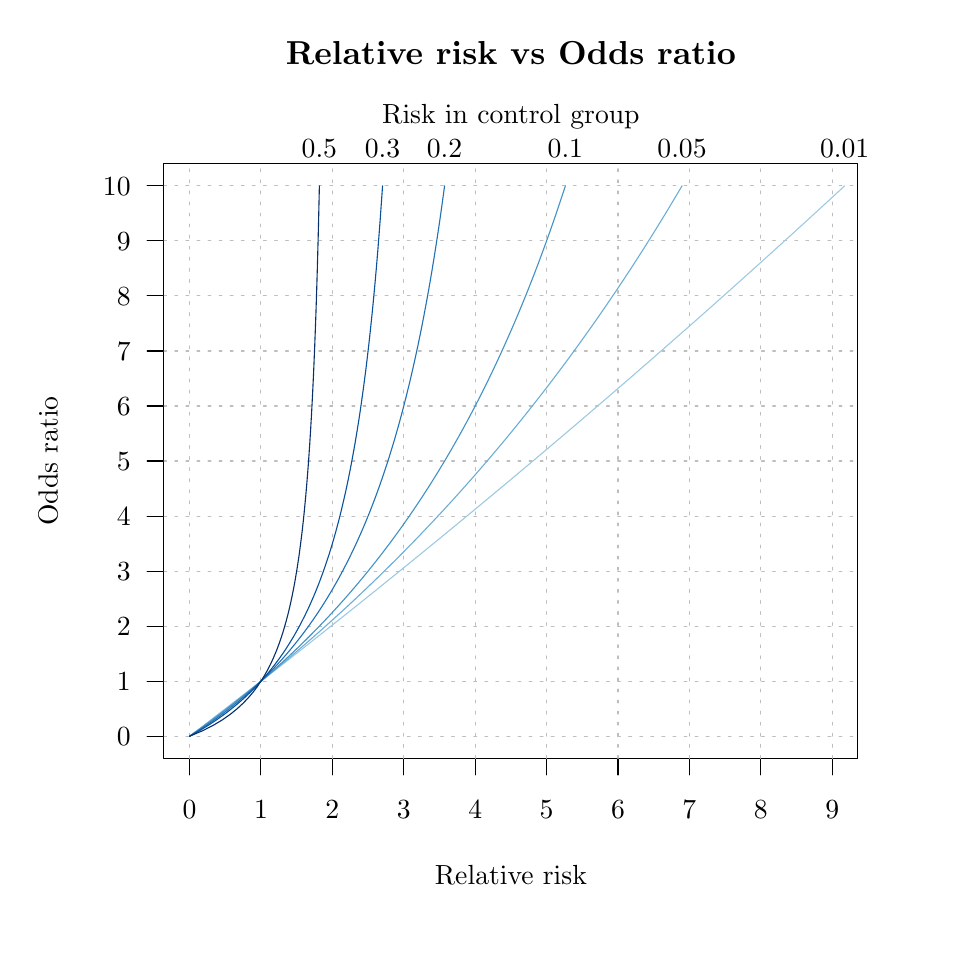
\begin{tikzpicture}[x=1pt,y=1pt]
\definecolor{fillColor}{RGB}{255,255,255}
\path[use as bounding box,fill=fillColor,fill opacity=0.00] (0,0) rectangle (325.21,325.21);
\begin{scope}
\path[clip] (  0.00,  0.00) rectangle (325.21,325.21);
\definecolor{drawColor}{RGB}{0,0,0}

\path[draw=drawColor,line width= 0.4pt,line join=round,line cap=round] ( 49.20, 61.20) --
	(300.01, 61.20) --
	(300.01,276.01) --
	( 49.20,276.01) --
	( 49.20, 61.20);
\end{scope}
\begin{scope}
\path[clip] (  0.00,  0.00) rectangle (325.21,325.21);
\definecolor{drawColor}{RGB}{0,0,0}

\node[text=drawColor,anchor=base,inner sep=0pt, outer sep=0pt, scale=  1.00] at (174.61, 15.60) {Relative risk};

\node[text=drawColor,rotate= 90.00,anchor=base,inner sep=0pt, outer sep=0pt, scale=  1.00] at ( 10.80,168.61) {Odds ratio};
\end{scope}
\begin{scope}
\path[clip] (  0.00,  0.00) rectangle (325.21,325.21);
\definecolor{drawColor}{RGB}{0,0,0}

\path[draw=drawColor,line width= 0.4pt,line join=round,line cap=round] ( 49.20, 69.16) -- ( 49.20,268.06);

\path[draw=drawColor,line width= 0.4pt,line join=round,line cap=round] ( 49.20, 69.16) -- ( 43.20, 69.16);

\path[draw=drawColor,line width= 0.4pt,line join=round,line cap=round] ( 49.20, 89.05) -- ( 43.20, 89.05);

\path[draw=drawColor,line width= 0.4pt,line join=round,line cap=round] ( 49.20,108.94) -- ( 43.20,108.94);

\path[draw=drawColor,line width= 0.4pt,line join=round,line cap=round] ( 49.20,128.83) -- ( 43.20,128.83);

\path[draw=drawColor,line width= 0.4pt,line join=round,line cap=round] ( 49.20,148.72) -- ( 43.20,148.72);

\path[draw=drawColor,line width= 0.4pt,line join=round,line cap=round] ( 49.20,168.61) -- ( 43.20,168.61);

\path[draw=drawColor,line width= 0.4pt,line join=round,line cap=round] ( 49.20,188.50) -- ( 43.20,188.50);

\path[draw=drawColor,line width= 0.4pt,line join=round,line cap=round] ( 49.20,208.39) -- ( 43.20,208.39);

\path[draw=drawColor,line width= 0.4pt,line join=round,line cap=round] ( 49.20,228.28) -- ( 43.20,228.28);

\path[draw=drawColor,line width= 0.4pt,line join=round,line cap=round] ( 49.20,248.17) -- ( 43.20,248.17);

\path[draw=drawColor,line width= 0.4pt,line join=round,line cap=round] ( 49.20,268.06) -- ( 43.20,268.06);

\node[text=drawColor,anchor=base east,inner sep=0pt, outer sep=0pt, scale=  1.00] at ( 37.20, 65.71) {0};

\node[text=drawColor,anchor=base east,inner sep=0pt, outer sep=0pt, scale=  1.00] at ( 37.20, 85.60) {1};

\node[text=drawColor,anchor=base east,inner sep=0pt, outer sep=0pt, scale=  1.00] at ( 37.20,105.49) {2};

\node[text=drawColor,anchor=base east,inner sep=0pt, outer sep=0pt, scale=  1.00] at ( 37.20,125.38) {3};

\node[text=drawColor,anchor=base east,inner sep=0pt, outer sep=0pt, scale=  1.00] at ( 37.20,145.27) {4};

\node[text=drawColor,anchor=base east,inner sep=0pt, outer sep=0pt, scale=  1.00] at ( 37.20,165.16) {5};

\node[text=drawColor,anchor=base east,inner sep=0pt, outer sep=0pt, scale=  1.00] at ( 37.20,185.05) {6};

\node[text=drawColor,anchor=base east,inner sep=0pt, outer sep=0pt, scale=  1.00] at ( 37.20,204.94) {7};

\node[text=drawColor,anchor=base east,inner sep=0pt, outer sep=0pt, scale=  1.00] at ( 37.20,224.83) {8};

\node[text=drawColor,anchor=base east,inner sep=0pt, outer sep=0pt, scale=  1.00] at ( 37.20,244.73) {9};

\node[text=drawColor,anchor=base east,inner sep=0pt, outer sep=0pt, scale=  1.00] at ( 37.20,264.62) {10};

\path[draw=drawColor,line width= 0.4pt,line join=round,line cap=round] ( 58.49, 61.20) -- (290.73, 61.20);

\path[draw=drawColor,line width= 0.4pt,line join=round,line cap=round] ( 58.49, 61.20) -- ( 58.49, 55.20);

\path[draw=drawColor,line width= 0.4pt,line join=round,line cap=round] ( 84.29, 61.20) -- ( 84.29, 55.20);

\path[draw=drawColor,line width= 0.4pt,line join=round,line cap=round] (110.10, 61.20) -- (110.10, 55.20);

\path[draw=drawColor,line width= 0.4pt,line join=round,line cap=round] (135.90, 61.20) -- (135.90, 55.20);

\path[draw=drawColor,line width= 0.4pt,line join=round,line cap=round] (161.71, 61.20) -- (161.71, 55.20);

\path[draw=drawColor,line width= 0.4pt,line join=round,line cap=round] (187.51, 61.20) -- (187.51, 55.20);

\path[draw=drawColor,line width= 0.4pt,line join=round,line cap=round] (213.31, 61.20) -- (213.31, 55.20);

\path[draw=drawColor,line width= 0.4pt,line join=round,line cap=round] (239.12, 61.20) -- (239.12, 55.20);

\path[draw=drawColor,line width= 0.4pt,line join=round,line cap=round] (264.92, 61.20) -- (264.92, 55.20);

\path[draw=drawColor,line width= 0.4pt,line join=round,line cap=round] (290.73, 61.20) -- (290.73, 55.20);

\node[text=drawColor,anchor=base,inner sep=0pt, outer sep=0pt, scale=  1.00] at ( 58.49, 39.60) {0};

\node[text=drawColor,anchor=base,inner sep=0pt, outer sep=0pt, scale=  1.00] at ( 84.29, 39.60) {1};

\node[text=drawColor,anchor=base,inner sep=0pt, outer sep=0pt, scale=  1.00] at (110.10, 39.60) {2};

\node[text=drawColor,anchor=base,inner sep=0pt, outer sep=0pt, scale=  1.00] at (135.90, 39.60) {3};

\node[text=drawColor,anchor=base,inner sep=0pt, outer sep=0pt, scale=  1.00] at (161.71, 39.60) {4};

\node[text=drawColor,anchor=base,inner sep=0pt, outer sep=0pt, scale=  1.00] at (187.51, 39.60) {5};

\node[text=drawColor,anchor=base,inner sep=0pt, outer sep=0pt, scale=  1.00] at (213.31, 39.60) {6};

\node[text=drawColor,anchor=base,inner sep=0pt, outer sep=0pt, scale=  1.00] at (239.12, 39.60) {7};

\node[text=drawColor,anchor=base,inner sep=0pt, outer sep=0pt, scale=  1.00] at (264.92, 39.60) {8};

\node[text=drawColor,anchor=base,inner sep=0pt, outer sep=0pt, scale=  1.00] at (290.73, 39.60) {9};
\end{scope}
\begin{scope}
\path[clip] ( 49.20, 61.20) rectangle (300.01,276.01);
\definecolor{drawColor}{RGB}{190,190,190}

\path[draw=drawColor,line width= 0.4pt,dash pattern=on 1pt off 3pt ,line join=round,line cap=round] ( 49.20, 69.16) -- (300.01, 69.16);

\path[draw=drawColor,line width= 0.4pt,dash pattern=on 1pt off 3pt ,line join=round,line cap=round] ( 49.20, 89.05) -- (300.01, 89.05);

\path[draw=drawColor,line width= 0.4pt,dash pattern=on 1pt off 3pt ,line join=round,line cap=round] ( 49.20,108.94) -- (300.01,108.94);

\path[draw=drawColor,line width= 0.4pt,dash pattern=on 1pt off 3pt ,line join=round,line cap=round] ( 49.20,128.83) -- (300.01,128.83);

\path[draw=drawColor,line width= 0.4pt,dash pattern=on 1pt off 3pt ,line join=round,line cap=round] ( 49.20,148.72) -- (300.01,148.72);

\path[draw=drawColor,line width= 0.4pt,dash pattern=on 1pt off 3pt ,line join=round,line cap=round] ( 49.20,168.61) -- (300.01,168.61);

\path[draw=drawColor,line width= 0.4pt,dash pattern=on 1pt off 3pt ,line join=round,line cap=round] ( 49.20,188.50) -- (300.01,188.50);

\path[draw=drawColor,line width= 0.4pt,dash pattern=on 1pt off 3pt ,line join=round,line cap=round] ( 49.20,208.39) -- (300.01,208.39);

\path[draw=drawColor,line width= 0.4pt,dash pattern=on 1pt off 3pt ,line join=round,line cap=round] ( 49.20,228.28) -- (300.01,228.28);

\path[draw=drawColor,line width= 0.4pt,dash pattern=on 1pt off 3pt ,line join=round,line cap=round] ( 49.20,248.17) -- (300.01,248.17);

\path[draw=drawColor,line width= 0.4pt,dash pattern=on 1pt off 3pt ,line join=round,line cap=round] ( 49.20,268.06) -- (300.01,268.06);

\path[draw=drawColor,line width= 0.4pt,dash pattern=on 1pt off 3pt ,line join=round,line cap=round] ( 58.49, 61.20) -- ( 58.49,276.01);

\path[draw=drawColor,line width= 0.4pt,dash pattern=on 1pt off 3pt ,line join=round,line cap=round] ( 84.29, 61.20) -- ( 84.29,276.01);

\path[draw=drawColor,line width= 0.4pt,dash pattern=on 1pt off 3pt ,line join=round,line cap=round] (110.10, 61.20) -- (110.10,276.01);

\path[draw=drawColor,line width= 0.4pt,dash pattern=on 1pt off 3pt ,line join=round,line cap=round] (135.90, 61.20) -- (135.90,276.01);

\path[draw=drawColor,line width= 0.4pt,dash pattern=on 1pt off 3pt ,line join=round,line cap=round] (161.71, 61.20) -- (161.71,276.01);

\path[draw=drawColor,line width= 0.4pt,dash pattern=on 1pt off 3pt ,line join=round,line cap=round] (187.51, 61.20) -- (187.51,276.01);

\path[draw=drawColor,line width= 0.4pt,dash pattern=on 1pt off 3pt ,line join=round,line cap=round] (213.31, 61.20) -- (213.31,276.01);

\path[draw=drawColor,line width= 0.4pt,dash pattern=on 1pt off 3pt ,line join=round,line cap=round] (239.12, 61.20) -- (239.12,276.01);

\path[draw=drawColor,line width= 0.4pt,dash pattern=on 1pt off 3pt ,line join=round,line cap=round] (264.92, 61.20) -- (264.92,276.01);

\path[draw=drawColor,line width= 0.4pt,dash pattern=on 1pt off 3pt ,line join=round,line cap=round] (290.73, 61.20) -- (290.73,276.01);
\end{scope}
\begin{scope}
\path[clip] (  0.00,  0.00) rectangle (325.21,325.21);
\definecolor{drawColor}{RGB}{0,0,0}

\node[text=drawColor,anchor=base,inner sep=0pt, outer sep=0pt, scale=  1.20] at (174.61,312.01) {\bfseries Relative risk vs Odds ratio};
\end{scope}
\begin{scope}
\path[clip] ( 49.20, 61.20) rectangle (300.01,276.01);
\definecolor{drawColor}{RGB}{158,202,225}

\path[draw=drawColor,line width= 0.4pt,line join=round,line cap=round] ( 58.49, 69.16) --
	( 61.09, 71.15) --
	( 63.69, 73.13) --
	( 66.29, 75.12) --
	( 68.87, 77.11) --
	( 71.46, 79.10) --
	( 74.03, 81.09) --
	( 76.61, 83.08) --
	( 79.17, 85.07) --
	( 81.74, 87.06) --
	( 84.29, 89.05) --
	( 86.85, 91.04) --
	( 89.39, 93.02) --
	( 91.93, 95.01) --
	( 94.47, 97.00) --
	( 97.00, 98.99) --
	( 99.53,100.98) --
	(102.05,102.97) --
	(104.57,104.96) --
	(107.08,106.95) --
	(109.59,108.94) --
	(112.09,110.93) --
	(114.59,112.91) --
	(117.08,114.90) --
	(119.56,116.89) --
	(122.05,118.88) --
	(124.52,120.87) --
	(127.00,122.86) --
	(129.46,124.85) --
	(131.93,126.84) --
	(134.38,128.83) --
	(136.84,130.82) --
	(139.28,132.80) --
	(141.73,134.79) --
	(144.17,136.78) --
	(146.60,138.77) --
	(149.03,140.76) --
	(151.45,142.75) --
	(153.87,144.74) --
	(156.29,146.73) --
	(158.70,148.72) --
	(161.10,150.71) --
	(163.51,152.70) --
	(165.90,154.68) --
	(168.29,156.67) --
	(170.68,158.66) --
	(173.06,160.65) --
	(175.44,162.64) --
	(177.81,164.63) --
	(180.18,166.62) --
	(182.55,168.61) --
	(184.91,170.60) --
	(187.26,172.59) --
	(189.61,174.57) --
	(191.96,176.56) --
	(194.30,178.55) --
	(196.64,180.54) --
	(198.97,182.53) --
	(201.30,184.52) --
	(203.62,186.51) --
	(205.94,188.50) --
	(208.26,190.49) --
	(210.57,192.48) --
	(212.87,194.46) --
	(215.17,196.45) --
	(217.47,198.44) --
	(219.76,200.43) --
	(222.05,202.42) --
	(224.34,204.41) --
	(226.62,206.40) --
	(228.89,208.39) --
	(231.16,210.38) --
	(233.43,212.37) --
	(235.69,214.36) --
	(237.95,216.34) --
	(240.21,218.33) --
	(242.46,220.32) --
	(244.70,222.31) --
	(246.95,224.30) --
	(249.18,226.29) --
	(251.42,228.28) --
	(253.65,230.27) --
	(255.87,232.26) --
	(258.09,234.25) --
	(260.31,236.23) --
	(262.52,238.22) --
	(264.73,240.21) --
	(266.93,242.20) --
	(269.13,244.19) --
	(271.33,246.18) --
	(273.52,248.17) --
	(275.71,250.16) --
	(277.90,252.15) --
	(280.08,254.14) --
	(282.25,256.12) --
	(284.42,258.11) --
	(286.59,260.10) --
	(288.76,262.09) --
	(290.92,264.08) --
	(293.07,266.07) --
	(295.22,268.06);
\end{scope}
\begin{scope}
\path[clip] (  0.00,  0.00) rectangle (325.21,325.21);
\definecolor{drawColor}{RGB}{0,0,0}

\node[text=drawColor,anchor=base,inner sep=0pt, outer sep=0pt, scale=  1.00] at (295.22,278.42) {0.01};
\end{scope}
\begin{scope}
\path[clip] ( 49.20, 61.20) rectangle (300.01,276.01);
\definecolor{drawColor}{RGB}{107,174,214}

\path[draw=drawColor,line width= 0.4pt,line join=round,line cap=round] ( 58.49, 69.16) --
	( 61.19, 71.15) --
	( 63.87, 73.13) --
	( 66.51, 75.12) --
	( 69.13, 77.11) --
	( 71.72, 79.10) --
	( 74.29, 81.09) --
	( 76.83, 83.08) --
	( 79.34, 85.07) --
	( 81.83, 87.06) --
	( 84.29, 89.05) --
	( 86.73, 91.04) --
	( 89.15, 93.02) --
	( 91.54, 95.01) --
	( 93.91, 97.00) --
	( 96.25, 98.99) --
	( 98.57,100.98) --
	(100.87,102.97) --
	(103.15,104.96) --
	(105.41,106.95) --
	(107.64,108.94) --
	(109.85,110.93) --
	(112.04,112.91) --
	(114.22,114.90) --
	(116.37,116.89) --
	(118.50,118.88) --
	(120.61,120.87) --
	(122.70,122.86) --
	(124.77,124.85) --
	(126.83,126.84) --
	(128.86,128.83) --
	(130.88,130.82) --
	(132.88,132.80) --
	(134.86,134.79) --
	(136.82,136.78) --
	(138.77,138.77) --
	(140.70,140.76) --
	(142.61,142.75) --
	(144.50,144.74) --
	(146.38,146.73) --
	(148.24,148.72) --
	(150.09,150.71) --
	(151.92,152.70) --
	(153.73,154.68) --
	(155.53,156.67) --
	(157.31,158.66) --
	(159.08,160.65) --
	(160.83,162.64) --
	(162.57,164.63) --
	(164.30,166.62) --
	(166.01,168.61) --
	(167.70,170.60) --
	(169.38,172.59) --
	(171.05,174.57) --
	(172.70,176.56) --
	(174.34,178.55) --
	(175.97,180.54) --
	(177.58,182.53) --
	(179.19,184.52) --
	(180.77,186.51) --
	(182.35,188.50) --
	(183.91,190.49) --
	(185.46,192.48) --
	(187.00,194.46) --
	(188.53,196.45) --
	(190.04,198.44) --
	(191.54,200.43) --
	(193.03,202.42) --
	(194.51,204.41) --
	(195.98,206.40) --
	(197.43,208.39) --
	(198.88,210.38) --
	(200.31,212.37) --
	(201.74,214.36) --
	(203.15,216.34) --
	(204.55,218.33) --
	(205.94,220.32) --
	(207.32,222.31) --
	(208.69,224.30) --
	(210.05,226.29) --
	(211.40,228.28) --
	(212.74,230.27) --
	(214.07,232.26) --
	(215.39,234.25) --
	(216.70,236.23) --
	(218.01,238.22) --
	(219.30,240.21) --
	(220.58,242.20) --
	(221.85,244.19) --
	(223.12,246.18) --
	(224.37,248.17) --
	(225.62,250.16) --
	(226.86,252.15) --
	(228.08,254.14) --
	(229.30,256.12) --
	(230.52,258.11) --
	(231.72,260.10) --
	(232.91,262.09) --
	(234.10,264.08) --
	(235.28,266.07) --
	(236.45,268.06);
\end{scope}
\begin{scope}
\path[clip] (  0.00,  0.00) rectangle (325.21,325.21);
\definecolor{drawColor}{RGB}{0,0,0}

\node[text=drawColor,anchor=base,inner sep=0pt, outer sep=0pt, scale=  1.00] at (236.45,278.42) {0.05};
\end{scope}
\begin{scope}
\path[clip] ( 49.20, 61.20) rectangle (300.01,276.01);
\definecolor{drawColor}{RGB}{66,146,198}

\path[draw=drawColor,line width= 0.4pt,line join=round,line cap=round] ( 58.49, 69.16) --
	( 61.33, 71.15) --
	( 64.10, 73.13) --
	( 66.81, 75.12) --
	( 69.47, 77.11) --
	( 72.07, 79.10) --
	( 74.62, 81.09) --
	( 77.11, 83.08) --
	( 79.55, 85.07) --
	( 81.95, 87.06) --
	( 84.29, 89.05) --
	( 86.59, 91.04) --
	( 88.85, 93.02) --
	( 91.06, 95.01) --
	( 93.23, 97.00) --
	( 95.35, 98.99) --
	( 97.44,100.98) --
	( 99.49,102.97) --
	(101.50,104.96) --
	(103.47,106.95) --
	(105.41,108.94) --
	(107.31,110.93) --
	(109.18,112.91) --
	(111.01,114.90) --
	(112.81,116.89) --
	(114.59,118.88) --
	(116.33,120.87) --
	(118.04,122.86) --
	(119.72,124.85) --
	(121.37,126.84) --
	(123.00,128.83) --
	(124.60,130.82) --
	(126.17,132.80) --
	(127.72,134.79) --
	(129.24,136.78) --
	(130.74,138.77) --
	(132.22,140.76) --
	(133.67,142.75) --
	(135.10,144.74) --
	(136.50,146.73) --
	(137.89,148.72) --
	(139.25,150.71) --
	(140.59,152.70) --
	(141.92,154.68) --
	(143.22,156.67) --
	(144.50,158.66) --
	(145.77,160.65) --
	(147.01,162.64) --
	(148.24,164.63) --
	(149.45,166.62) --
	(150.65,168.61) --
	(151.82,170.60) --
	(152.98,172.59) --
	(154.13,174.57) --
	(155.25,176.56) --
	(156.37,178.55) --
	(157.46,180.54) --
	(158.55,182.53) --
	(159.61,184.52) --
	(160.67,186.51) --
	(161.71,188.50) --
	(162.73,190.49) --
	(163.74,192.48) --
	(164.74,194.46) --
	(165.73,196.45) --
	(166.70,198.44) --
	(167.66,200.43) --
	(168.61,202.42) --
	(169.54,204.41) --
	(170.47,206.40) --
	(171.38,208.39) --
	(172.28,210.38) --
	(173.17,212.37) --
	(174.05,214.36) --
	(174.92,216.34) --
	(175.78,218.33) --
	(176.63,220.32) --
	(177.47,222.31) --
	(178.29,224.30) --
	(179.11,226.29) --
	(179.92,228.28) --
	(180.72,230.27) --
	(181.51,232.26) --
	(182.29,234.25) --
	(183.06,236.23) --
	(183.82,238.22) --
	(184.58,240.21) --
	(185.32,242.20) --
	(186.06,244.19) --
	(186.79,246.18) --
	(187.51,248.17) --
	(188.22,250.16) --
	(188.93,252.15) --
	(189.62,254.14) --
	(190.31,256.12) --
	(191.00,258.11) --
	(191.67,260.10) --
	(192.34,262.09) --
	(193.00,264.08) --
	(193.65,266.07) --
	(194.30,268.06);
\end{scope}
\begin{scope}
\path[clip] (  0.00,  0.00) rectangle (325.21,325.21);
\definecolor{drawColor}{RGB}{0,0,0}

\node[text=drawColor,anchor=base,inner sep=0pt, outer sep=0pt, scale=  1.00] at (194.30,278.42) {0.1};
\end{scope}
\begin{scope}
\path[clip] ( 49.20, 61.20) rectangle (300.01,276.01);
\definecolor{drawColor}{RGB}{33,113,181}

\path[draw=drawColor,line width= 0.4pt,line join=round,line cap=round] ( 58.49, 69.16) --
	( 61.64, 71.15) --
	( 64.63, 73.13) --
	( 67.49, 75.12) --
	( 70.22, 77.11) --
	( 72.83, 79.10) --
	( 75.32, 81.09) --
	( 77.71, 83.08) --
	( 79.99, 85.07) --
	( 82.19, 87.06) --
	( 84.29, 89.05) --
	( 86.32, 91.04) --
	( 88.26, 93.02) --
	( 90.14, 95.01) --
	( 91.94, 97.00) --
	( 93.68, 98.99) --
	( 95.35,100.98) --
	( 96.97,102.97) --
	( 98.53,104.96) --
	(100.04,106.95) --
	(101.50,108.94) --
	(102.91,110.93) --
	(104.27,112.91) --
	(105.59,114.90) --
	(106.87,116.89) --
	(108.11,118.88) --
	(109.32,120.87) --
	(110.48,122.86) --
	(111.62,124.85) --
	(112.72,126.84) --
	(113.78,128.83) --
	(114.82,130.82) --
	(115.83,132.80) --
	(116.81,134.79) --
	(117.77,136.78) --
	(118.70,138.77) --
	(119.60,140.76) --
	(120.49,142.75) --
	(121.35,144.74) --
	(122.18,146.73) --
	(123.00,148.72) --
	(123.80,150.71) --
	(124.57,152.70) --
	(125.33,154.68) --
	(126.07,156.67) --
	(126.79,158.66) --
	(127.50,160.65) --
	(128.19,162.64) --
	(128.86,164.63) --
	(129.52,166.62) --
	(130.17,168.61) --
	(130.80,170.60) --
	(131.41,172.59) --
	(132.02,174.57) --
	(132.61,176.56) --
	(133.19,178.55) --
	(133.75,180.54) --
	(134.31,182.53) --
	(134.85,184.52) --
	(135.38,186.51) --
	(135.90,188.50) --
	(136.41,190.49) --
	(136.91,192.48) --
	(137.40,194.46) --
	(137.89,196.45) --
	(138.36,198.44) --
	(138.82,200.43) --
	(139.28,202.42) --
	(139.72,204.41) --
	(140.16,206.40) --
	(140.59,208.39) --
	(141.02,210.38) --
	(141.43,212.37) --
	(141.84,214.36) --
	(142.24,216.34) --
	(142.63,218.33) --
	(143.02,220.32) --
	(143.40,222.31) --
	(143.77,224.30) --
	(144.14,226.29) --
	(144.50,228.28) --
	(144.86,230.27) --
	(145.21,232.26) --
	(145.55,234.25) --
	(145.89,236.23) --
	(146.22,238.22) --
	(146.55,240.21) --
	(146.87,242.20) --
	(147.19,244.19) --
	(147.50,246.18) --
	(147.81,248.17) --
	(148.11,250.16) --
	(148.41,252.15) --
	(148.71,254.14) --
	(149.00,256.12) --
	(149.28,258.11) --
	(149.56,260.10) --
	(149.84,262.09) --
	(150.11,264.08) --
	(150.38,266.07) --
	(150.65,268.06);
\end{scope}
\begin{scope}
\path[clip] (  0.00,  0.00) rectangle (325.21,325.21);
\definecolor{drawColor}{RGB}{0,0,0}

\node[text=drawColor,anchor=base,inner sep=0pt, outer sep=0pt, scale=  1.00] at (150.65,278.42) {0.2};
\end{scope}
\begin{scope}
\path[clip] ( 49.20, 61.20) rectangle (300.01,276.01);
\definecolor{drawColor}{RGB}{8,81,156}

\path[draw=drawColor,line width= 0.4pt,line join=round,line cap=round] ( 58.49, 69.16) --
	( 62.02, 71.15) --
	( 65.28, 73.13) --
	( 68.29, 75.12) --
	( 71.08, 77.11) --
	( 73.67, 79.10) --
	( 76.08, 81.09) --
	( 78.34, 83.08) --
	( 80.45, 85.07) --
	( 82.43, 87.06) --
	( 84.29, 89.05) --
	( 86.05, 91.04) --
	( 87.70, 93.02) --
	( 89.26, 95.01) --
	( 90.74, 97.00) --
	( 92.15, 98.99) --
	( 93.48,100.98) --
	( 94.74,102.97) --
	( 95.95,104.96) --
	( 97.09,106.95) --
	( 98.19,108.94) --
	( 99.23,110.93) --
	(100.23,112.91) --
	(101.19,114.90) --
	(102.10,116.89) --
	(102.98,118.88) --
	(103.82,120.87) --
	(104.63,122.86) --
	(105.41,124.85) --
	(106.15,126.84) --
	(106.87,128.83) --
	(107.56,130.82) --
	(108.23,132.80) --
	(108.88,134.79) --
	(109.50,136.78) --
	(110.10,138.77) --
	(110.68,140.76) --
	(111.24,142.75) --
	(111.78,144.74) --
	(112.31,146.73) --
	(112.81,148.72) --
	(113.31,150.71) --
	(113.78,152.70) --
	(114.25,154.68) --
	(114.70,156.67) --
	(115.13,158.66) --
	(115.56,160.65) --
	(115.97,162.64) --
	(116.37,164.63) --
	(116.76,166.62) --
	(117.13,168.61) --
	(117.50,170.60) --
	(117.86,172.59) --
	(118.21,174.57) --
	(118.55,176.56) --
	(118.88,178.55) --
	(119.20,180.54) --
	(119.52,182.53) --
	(119.83,184.52) --
	(120.13,186.51) --
	(120.42,188.50) --
	(120.70,190.49) --
	(120.98,192.48) --
	(121.26,194.46) --
	(121.52,196.45) --
	(121.78,198.44) --
	(122.04,200.43) --
	(122.29,202.42) --
	(122.53,204.41) --
	(122.77,206.40) --
	(123.00,208.39) --
	(123.23,210.38) --
	(123.45,212.37) --
	(123.67,214.36) --
	(123.88,216.34) --
	(124.09,218.33) --
	(124.30,220.32) --
	(124.50,222.31) --
	(124.70,224.30) --
	(124.89,226.29) --
	(125.08,228.28) --
	(125.27,230.27) --
	(125.45,232.26) --
	(125.63,234.25) --
	(125.80,236.23) --
	(125.98,238.22) --
	(126.15,240.21) --
	(126.31,242.20) --
	(126.48,244.19) --
	(126.64,246.18) --
	(126.79,248.17) --
	(126.95,250.16) --
	(127.10,252.15) --
	(127.25,254.14) --
	(127.40,256.12) --
	(127.54,258.11) --
	(127.68,260.10) --
	(127.82,262.09) --
	(127.96,264.08) --
	(128.10,266.07) --
	(128.23,268.06);
\end{scope}
\begin{scope}
\path[clip] (  0.00,  0.00) rectangle (325.21,325.21);
\definecolor{drawColor}{RGB}{0,0,0}

\node[text=drawColor,anchor=base,inner sep=0pt, outer sep=0pt, scale=  1.00] at (128.23,278.42) {0.3};
\end{scope}
\begin{scope}
\path[clip] ( 49.20, 61.20) rectangle (300.01,276.01);
\definecolor{drawColor}{RGB}{8,48,107}

\path[draw=drawColor,line width= 0.4pt,line join=round,line cap=round] ( 58.49, 69.16) --
	( 63.18, 71.15) --
	( 67.09, 73.13) --
	( 70.40, 75.12) --
	( 73.23, 77.11) --
	( 75.69, 79.10) --
	( 77.84, 81.09) --
	( 79.74, 83.08) --
	( 81.43, 85.07) --
	( 82.94, 87.06) --
	( 84.29, 89.05) --
	( 85.52, 91.04) --
	( 86.64, 93.02) --
	( 87.66, 95.01) --
	( 88.59, 97.00) --
	( 89.45, 98.99) --
	( 90.25,100.98) --
	( 90.98,102.97) --
	( 91.67,104.96) --
	( 92.30,106.95) --
	( 92.89,108.94) --
	( 93.45,110.93) --
	( 93.97,112.91) --
	( 94.46,114.90) --
	( 94.92,116.89) --
	( 95.35,118.88) --
	( 95.76,120.87) --
	( 96.15,122.86) --
	( 96.52,124.85) --
	( 96.86,126.84) --
	( 97.20,128.83) --
	( 97.51,130.82) --
	( 97.81,132.80) --
	( 98.10,134.79) --
	( 98.37,136.78) --
	( 98.63,138.77) --
	( 98.88,140.76) --
	( 99.12,142.75) --
	( 99.35,144.74) --
	( 99.57,146.73) --
	( 99.78,148.72) --
	( 99.98,150.71) --
	(100.17,152.70) --
	(100.36,154.68) --
	(100.54,156.67) --
	(100.71,158.66) --
	(100.88,160.65) --
	(101.04,162.64) --
	(101.20,164.63) --
	(101.35,166.62) --
	(101.50,168.61) --
	(101.64,170.60) --
	(101.77,172.59) --
	(101.91,174.57) --
	(102.03,176.56) --
	(102.16,178.55) --
	(102.28,180.54) --
	(102.39,182.53) --
	(102.51,184.52) --
	(102.62,186.51) --
	(102.72,188.50) --
	(102.83,190.49) --
	(102.93,192.48) --
	(103.03,194.46) --
	(103.12,196.45) --
	(103.22,198.44) --
	(103.31,200.43) --
	(103.40,202.42) --
	(103.48,204.41) --
	(103.56,206.40) --
	(103.65,208.39) --
	(103.73,210.38) --
	(103.80,212.37) --
	(103.88,214.36) --
	(103.95,216.34) --
	(104.03,218.33) --
	(104.10,220.32) --
	(104.17,222.31) --
	(104.23,224.30) --
	(104.30,226.29) --
	(104.36,228.28) --
	(104.43,230.27) --
	(104.49,232.26) --
	(104.55,234.25) --
	(104.61,236.23) --
	(104.67,238.22) --
	(104.72,240.21) --
	(104.78,242.20) --
	(104.83,244.19) --
	(104.88,246.18) --
	(104.94,248.17) --
	(104.99,250.16) --
	(105.04,252.15) --
	(105.09,254.14) --
	(105.14,256.12) --
	(105.18,258.11) --
	(105.23,260.10) --
	(105.27,262.09) --
	(105.32,264.08) --
	(105.36,266.07) --
	(105.41,268.06);
\end{scope}
\begin{scope}
\path[clip] (  0.00,  0.00) rectangle (325.21,325.21);
\definecolor{drawColor}{RGB}{0,0,0}

\node[text=drawColor,anchor=base,inner sep=0pt, outer sep=0pt, scale=  1.00] at (105.41,278.42) {0.5};

\node[text=drawColor,anchor=base,inner sep=0pt, outer sep=0pt, scale=  1.00] at (174.61,290.41) {Risk in control group};
\end{scope}
\end{tikzpicture}
}}
\end{center}
\end{frame}



\subsection{Diagnostic tests}

%---------------------------------------------------------------------slide----
\begin{frame}
\frametitle{Diagnostic tests}
In Epidemiology it is common to use diagnostic test to diagnose diseases.

In general, diagnostic tests are not fully reliable and have some risk of misdiagnosis as it is represented in the table below.

\begin{center}
\begin{tabular}{|m{2.5cm}|m{3cm}<{\centering}|m{3cm}<{\centering}|}
\cline{2-3}
\multicolumn{1}{c|}{} & Presence of disease $D$ & Absence of disease $\overline D$\\ \hline
Test outcome\newline positive $+$ & \textcolor{green}{True Positive}\newline $TP$ & \textcolor{red}{False
Positive}\newline $FP$\\ \hline Test outcome\newline negative $-$ & \textcolor{red}{False Negative}\newline $FN$ &
\textcolor{green}{True Negative}\newline $TN$\\ \hline
\end{tabular}
\end{center}
\end{frame}


%---------------------------------------------------------------------slide----
\begin{frame}
\frametitle{Sensitivity and specificity of a diagnostic test}
The performance of a diagnostic test depends on the following two probabilities.
\begin{definition}[Sensitivity]
The \emph{sensitivity} of a diagnostic test is the proportion of positive outcomes in persons with the disease 
\[
P(+|D)=\frac{TP}{TP+FN}
\]
\end{definition}

\begin{definition}[Specificity]
The \emph{specificity} of a diagnostic test is the proportion of negative outcomes in persons without the disease
\[
P(-|\overline{D})=\frac{TN}{TN+FP}
\]
\end{definition}
\end{frame}


%---------------------------------------------------------------------slide----
\begin{frame}
\frametitle{Sensitivity and specificity interpretation}
Usually, there is a trade-off between sensitivity and specificity.  

A test with high sensitivity will detect the disease in most sick persons, but it will produce also more false positives than a less sensitive test. 
This way, a positive outcome in a test with high sensitivity is not useful for confirming the disease, but a negative outcome is useful for ruling out the disease, since it rarely give negative outcomes in sick people.

On the other hand, a test with a high specificity will rule out the disease in most healthy persons, but it will produce also more false negatives than a less specific test. 
Thus, a negative outcome in a test with high specificity is not useful for ruling out the disease, but a positive is useful to confirm the disease, since it rarely give positive outcomes in healthy people.  
\end{frame}


%---------------------------------------------------------------------slide----
\begin{frame}
\frametitle{Sensitivity and specificity interpretation}
Deciding on a test with greater sensitivity or a test with greater specificity depends on the type of disease and the
goal of the test.
In general, we will use a sensitive test when:
\begin{itemize}
\item The disease is serious and it is important to detect it. 
\item The disease is curable. 
\item The false positives do not provoke serious traumas.
\end{itemize}

And we will use a specific test when:
\begin{itemize}
\item The disease is important but difficult or impossible to cure.
\item The false positives provoke serious traumas. 
\item The treatment of false positives can have dangerous consequences.  
\end{itemize}
\end{frame}


%---------------------------------------------------------------------slide----
\begin{frame}
\frametitle{Predictive values of a diagnostic test}
But the most important aspect of a diagnostic test is its predictive power, that is measured with the following two posterior probabilities.
\begin{definition}[Positive predictive value $PPV$]
The \emph{positive predictive value} of a diagnostic test is the proportion of persons with the disease to persons with a positive outcome
\[
P(D|+) = \frac{TP}{TP+FP}
\]
\end{definition}

\begin{definition}[Negative predictive value $NPV$]
The \emph{negative predictive value} of a diagnostic test is the proportion of persons without the disease to persons with a negative outcome 
\[
P(\overline{D}|-) = \frac{TN}{TN+FN}
\]
\end{definition}
\end{frame}


%---------------------------------------------------------------------slide----
\begin{frame}
\frametitle{Predictive values interpretation}
Positive and negative predictive values allow to confirm or to rule out the disease, respectively, if they reach at least a threshold of $0.5$.
\[
\begin{array}{rcl}
PPV>0.5 & \Rightarrow & \mbox{Disease diagnostic}\\
NPV>0.5 & \Rightarrow & \mbox{Not disease diagnostic} 
\end{array}
\]

However, these probabilities depends on prevalence of the disease $P(D)$.
They can be calculated from the sensitivity and the specificity of the diagnostic test using the Bayes theorem.

\begin{align*}
PPV=P(D|+) &= \frac{P(D)P(+|D)}{P(D)P(+|D)+P(\overline{D})P(+|\overline{D})}\\
NPV=P(\overline{D}|-) &= \frac{P(\overline{D})P(-|\overline{D})}{P(D)P(-|D)+P(\overline{D})P(-|\overline{D})}
%  = \frac{\mbox{Prevalence}\cdot
% \mbox{Sensitivity}}{\mbox{Prevalence}\cdot \mbox{Sensitivity}+(1-\mbox{Prevalence})\cdot (1-\mbox{Specificity})}
\end{align*}

Thus, with frequent diseases, the positive predictive value increases, and with rare diseases, the negative predictive value increases. 
\end{frame}


% ---------------------------------------------------------------------slide----
\begin{frame}
\frametitle{Diagnostic tests}
\framesubtitle{Example}
A diagnostic test for the flu has been tried in a random sample of 1000 persons.
The results are summarized in the table below.
\begin{center}
\begin{tabular}{|m{2.5cm}|m{3cm}<{\centering}|m{3cm}<{\centering}|}
\cline{2-3}
\multicolumn{1}{c|}{} & Presence of flu $D$ & Absence of flu $\overline D$\\ \hline
Test outcome $+$ & 95 & 90 \\
\hline
Test outcome $-$ & 5 & 810 \\
\hline
\end{tabular}
\end{center}

According to this sample, the prevalence of the flu can be estimated as
\[
P(D) = \frac{95+5}{1000} = 0.1.
\] 

The sensitivity of this diagnostic test is
\[
P(+|D) = \frac{95}{95+5}= 0.95. 
\] 

And the specificity is 
\[
P(-|\overline{D}) = \frac{810}{90+810}=0.9.
\]
\end{frame}


% ---------------------------------------------------------------------slide----
\begin{frame}
\frametitle{Diagnostic tests}
\framesubtitle{Example cont.}
The predictive positive value of the diagnostic test is
\[
PPV = P(D|+) = \frac{95}{95+90} = 0.5135.
\]

As this value is over $0.5$, this means that we will diagnose the flu if the outcome of the test is positive. 
However, the confidence in the diagnostic will be low, as this value is pretty close to $0.5$.

On the other hand, the predictive negative value is 
\[
NPV = P(\overline{D}|-) = \frac{810}{5+810} = 0.9939. 
\]

As this value is almost 1, that means that is almost sure that a person does not have the flu if he or she gets a
negative outcome in the test. 

Thus, this test is a powerful test to rule out the flu, but not so powerful to confirm it.    
\end{frame}


%---------------------------------------------------------------------slide----
\begin{frame}
\frametitle{Likelihood ratios of a diagnostic test}
The following measures are usually derived from sensitivity and specificity.
\begin{definition}[Positive likelihood ratio $LR+$]
The \emph{positive likelihood ratio} of a diagnostic test is the ratio between the probability of positive outcomes in
persons with the disease and healthy persons respectively,
\[
LR+=\frac{P(+|D)}{P(+|\overline{D})} = \frac{\mbox{Sensitivity}}{1-\mbox{Specificity}}
\]
\end{definition}

\begin{definition}[Negative likelihood ratio $LR-$]
The \emph{negative likelihood ratio} of a diagnostic test is the ratio between the probability of negative outcomes in
persons with the disease and healthy persons respectively,
\[
LR-=\frac{P(-|D)}{P(-|\overline{D})} = \frac{1-\mbox{Sensitivity}}{\mbox{Specificity}}
\]
\end{definition}
\end{frame}


%---------------------------------------------------------------------slide----
\begin{frame}
\frametitle{Likelihood ratios interpretation}
Positive likelihood ratio can be interpreted as the number of times that a positive outcome is more probable in people
with the disease than in people without it. 

On the other hand, negative likelihood ratio can be interpreted as the number of times that a negative outcome is more
probable in people with the disease than in people without it. 

Post-test probabilities can be calculated from pre-test probabilities through likelihood ratios.

\[
P(D|+) = \frac{P(D)P(+|D)}{P(D)P(+|D)+P(\overline{D})P(+|\overline{D})} = \frac{P(D)LR+}{1-P(D)+P(D)LR+}
\]

Thus, 
\begin{itemize}
\item A likelihood ratio greater than 1 increases the probability of disease.
\item A likelihood ratio less than 1 decreases the probability of disease.
\item A likelihood ratio 1 does not change the pre-test probability. 
\end{itemize}
\end{frame}


%---------------------------------------------------------------------slide----
\begin{frame}
\frametitle{Likelihood ratios interpretation}
\begin{center}
\tikzsetnextfilename{probability/likelihood_ratios}
\mode<article>{\resizebox{0.6\textwidth}{!}{% Created by tikzDevice version 0.10.1 on 2016-03-21 19:09:18
% !TEX encoding = UTF-8 Unicode
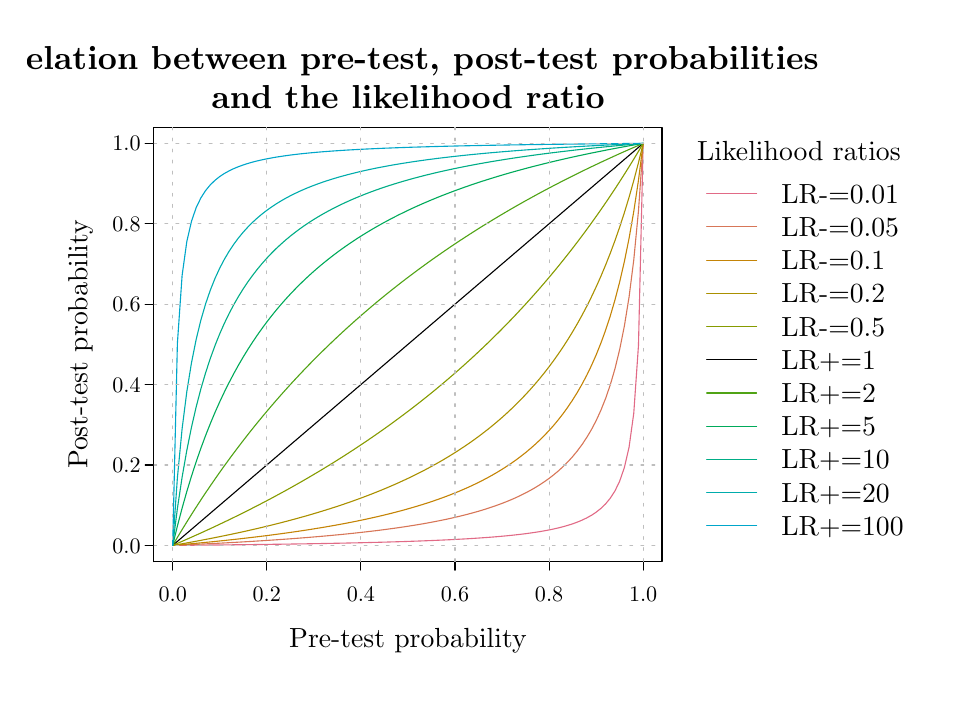
\begin{tikzpicture}[x=1pt,y=1pt]
\definecolor{fillColor}{RGB}{255,255,255}
\path[use as bounding box,fill=fillColor,fill opacity=0.00] (0,0) rectangle (325.21,238.49);
\begin{scope}
\path[clip] ( 45.60, 45.60) rectangle (229.21,202.49);
\definecolor{drawColor}{RGB}{0,0,0}

\path[draw=drawColor,line width= 0.4pt,line join=round,line cap=round] ( 52.40, 51.41) --
	( 54.10, 52.86) --
	( 55.80, 54.32) --
	( 57.50, 55.77) --
	( 59.20, 57.22) --
	( 60.90, 58.67) --
	( 62.60, 60.13) --
	( 64.30, 61.58) --
	( 66.00, 63.03) --
	( 67.70, 64.49) --
	( 69.40, 65.94) --
	( 71.10, 67.39) --
	( 72.80, 68.84) --
	( 74.50, 70.30) --
	( 76.20, 71.75) --
	( 77.90, 73.20) --
	( 79.60, 74.65) --
	( 81.30, 76.11) --
	( 83.00, 77.56) --
	( 84.70, 79.01) --
	( 86.40, 80.46) --
	( 88.10, 81.92) --
	( 89.80, 83.37) --
	( 91.50, 84.82) --
	( 93.20, 86.28) --
	( 94.90, 87.73) --
	( 96.60, 89.18) --
	( 98.30, 90.63) --
	(100.00, 92.09) --
	(101.70, 93.54) --
	(103.40, 94.99) --
	(105.10, 96.44) --
	(106.80, 97.90) --
	(108.51, 99.35) --
	(110.21,100.80) --
	(111.91,102.26) --
	(113.61,103.71) --
	(115.31,105.16) --
	(117.01,106.61) --
	(118.71,108.07) --
	(120.41,109.52) --
	(122.11,110.97) --
	(123.81,112.42) --
	(125.51,113.88) --
	(127.21,115.33) --
	(128.91,116.78) --
	(130.61,118.23) --
	(132.31,119.69) --
	(134.01,121.14) --
	(135.71,122.59) --
	(137.41,124.05) --
	(139.11,125.50) --
	(140.81,126.95) --
	(142.51,128.40) --
	(144.21,129.86) --
	(145.91,131.31) --
	(147.61,132.76) --
	(149.31,134.21) --
	(151.01,135.67) --
	(152.71,137.12) --
	(154.41,138.57) --
	(156.11,140.03) --
	(157.81,141.48) --
	(159.51,142.93) --
	(161.21,144.38) --
	(162.91,145.84) --
	(164.61,147.29) --
	(166.31,148.74) --
	(168.01,150.19) --
	(169.71,151.65) --
	(171.41,153.10) --
	(173.11,154.55) --
	(174.81,156.00) --
	(176.51,157.46) --
	(178.21,158.91) --
	(179.91,160.36) --
	(181.61,161.82) --
	(183.31,163.27) --
	(185.01,164.72) --
	(186.71,166.17) --
	(188.41,167.63) --
	(190.11,169.08) --
	(191.81,170.53) --
	(193.51,171.98) --
	(195.21,173.44) --
	(196.91,174.89) --
	(198.61,176.34) --
	(200.31,177.80) --
	(202.01,179.25) --
	(203.71,180.70) --
	(205.41,182.15) --
	(207.11,183.61) --
	(208.81,185.06) --
	(210.51,186.51) --
	(212.21,187.96) --
	(213.91,189.42) --
	(215.61,190.87) --
	(217.31,192.32) --
	(219.01,193.77) --
	(220.71,195.23) --
	(222.41,196.68);
\end{scope}
\begin{scope}
\path[clip] (  0.00,  0.00) rectangle (325.21,238.49);
\definecolor{drawColor}{RGB}{0,0,0}

\path[draw=drawColor,line width= 0.4pt,line join=round,line cap=round] ( 52.40, 45.60) -- (222.41, 45.60);

\path[draw=drawColor,line width= 0.4pt,line join=round,line cap=round] ( 52.40, 45.60) -- ( 52.40, 42.46);

\path[draw=drawColor,line width= 0.4pt,line join=round,line cap=round] ( 86.40, 45.60) -- ( 86.40, 42.46);

\path[draw=drawColor,line width= 0.4pt,line join=round,line cap=round] (120.41, 45.60) -- (120.41, 42.46);

\path[draw=drawColor,line width= 0.4pt,line join=round,line cap=round] (154.41, 45.60) -- (154.41, 42.46);

\path[draw=drawColor,line width= 0.4pt,line join=round,line cap=round] (188.41, 45.60) -- (188.41, 42.46);

\path[draw=drawColor,line width= 0.4pt,line join=round,line cap=round] (222.41, 45.60) -- (222.41, 42.46);

\node[text=drawColor,anchor=base,inner sep=0pt, outer sep=0pt, scale=  0.80] at ( 52.40, 31.20) {0.0};

\node[text=drawColor,anchor=base,inner sep=0pt, outer sep=0pt, scale=  0.80] at ( 86.40, 31.20) {0.2};

\node[text=drawColor,anchor=base,inner sep=0pt, outer sep=0pt, scale=  0.80] at (120.41, 31.20) {0.4};

\node[text=drawColor,anchor=base,inner sep=0pt, outer sep=0pt, scale=  0.80] at (154.41, 31.20) {0.6};

\node[text=drawColor,anchor=base,inner sep=0pt, outer sep=0pt, scale=  0.80] at (188.41, 31.20) {0.8};

\node[text=drawColor,anchor=base,inner sep=0pt, outer sep=0pt, scale=  0.80] at (222.41, 31.20) {1.0};

\path[draw=drawColor,line width= 0.4pt,line join=round,line cap=round] ( 45.60, 51.41) -- ( 45.60,196.68);

\path[draw=drawColor,line width= 0.4pt,line join=round,line cap=round] ( 45.60, 51.41) -- ( 42.46, 51.41);

\path[draw=drawColor,line width= 0.4pt,line join=round,line cap=round] ( 45.60, 80.46) -- ( 42.46, 80.46);

\path[draw=drawColor,line width= 0.4pt,line join=round,line cap=round] ( 45.60,109.52) -- ( 42.46,109.52);

\path[draw=drawColor,line width= 0.4pt,line join=round,line cap=round] ( 45.60,138.57) -- ( 42.46,138.57);

\path[draw=drawColor,line width= 0.4pt,line join=round,line cap=round] ( 45.60,167.63) -- ( 42.46,167.63);

\path[draw=drawColor,line width= 0.4pt,line join=round,line cap=round] ( 45.60,196.68) -- ( 42.46,196.68);

\node[text=drawColor,anchor=base east,inner sep=0pt, outer sep=0pt, scale=  0.80] at ( 40.80, 48.66) {0.0};

\node[text=drawColor,anchor=base east,inner sep=0pt, outer sep=0pt, scale=  0.80] at ( 40.80, 77.71) {0.2};

\node[text=drawColor,anchor=base east,inner sep=0pt, outer sep=0pt, scale=  0.80] at ( 40.80,106.76) {0.4};

\node[text=drawColor,anchor=base east,inner sep=0pt, outer sep=0pt, scale=  0.80] at ( 40.80,135.82) {0.6};

\node[text=drawColor,anchor=base east,inner sep=0pt, outer sep=0pt, scale=  0.80] at ( 40.80,164.87) {0.8};

\node[text=drawColor,anchor=base east,inner sep=0pt, outer sep=0pt, scale=  0.80] at ( 40.80,193.93) {1.0};

\path[draw=drawColor,line width= 0.4pt,line join=round,line cap=round] ( 45.60, 45.60) --
	(229.21, 45.60) --
	(229.21,202.49) --
	( 45.60,202.49) --
	( 45.60, 45.60);
\end{scope}
\begin{scope}
\path[clip] (  0.00,  0.00) rectangle (325.21,238.49);
\definecolor{drawColor}{RGB}{0,0,0}

\node[text=drawColor,anchor=base,inner sep=0pt, outer sep=0pt, scale=  1.20] at (137.41,223.55) {\bfseries Relation between pre-test, post-test probabilities};

\node[text=drawColor,anchor=base,inner sep=0pt, outer sep=0pt, scale=  1.20] at (137.41,209.15) {\bfseries  and the likelihood ratio};

\node[text=drawColor,anchor=base,inner sep=0pt, outer sep=0pt, scale=  1.00] at (137.41, 14.40) {Pre-test probability};

\node[text=drawColor,rotate= 90.00,anchor=base,inner sep=0pt, outer sep=0pt, scale=  1.00] at ( 21.60,124.05) {Post-test probability};
\end{scope}
\begin{scope}
\path[clip] ( 45.60, 45.60) rectangle (229.21,202.49);
\definecolor{drawColor}{RGB}{225,106,134}

\path[draw=drawColor,line width= 0.4pt,line join=round,line cap=round] ( 52.40, 51.41) --
	( 54.10, 51.43) --
	( 55.80, 51.44) --
	( 57.50, 51.46) --
	( 59.20, 51.47) --
	( 60.90, 51.49) --
	( 62.60, 51.50) --
	( 64.30, 51.52) --
	( 66.00, 51.54) --
	( 67.70, 51.55) --
	( 69.40, 51.57) --
	( 71.10, 51.59) --
	( 72.80, 51.61) --
	( 74.50, 51.63) --
	( 76.20, 51.65) --
	( 77.90, 51.67) --
	( 79.60, 51.69) --
	( 81.30, 51.71) --
	( 83.00, 51.73) --
	( 84.70, 51.75) --
	( 86.40, 51.77) --
	( 88.10, 51.80) --
	( 89.80, 51.82) --
	( 91.50, 51.84) --
	( 93.20, 51.87) --
	( 94.90, 51.89) --
	( 96.60, 51.92) --
	( 98.30, 51.95) --
	(100.00, 51.97) --
	(101.70, 52.00) --
	(103.40, 52.03) --
	(105.10, 52.06) --
	(106.80, 52.09) --
	(108.51, 52.12) --
	(110.21, 52.16) --
	(111.91, 52.19) --
	(113.61, 52.22) --
	(115.31, 52.26) --
	(117.01, 52.30) --
	(118.71, 52.33) --
	(120.41, 52.37) --
	(122.11, 52.41) --
	(123.81, 52.46) --
	(125.51, 52.50) --
	(127.21, 52.54) --
	(128.91, 52.59) --
	(130.61, 52.64) --
	(132.31, 52.69) --
	(134.01, 52.74) --
	(135.71, 52.79) --
	(137.41, 52.85) --
	(139.11, 52.91) --
	(140.81, 52.97) --
	(142.51, 53.03) --
	(144.21, 53.10) --
	(145.91, 53.16) --
	(147.61, 53.24) --
	(149.31, 53.31) --
	(151.01, 53.39) --
	(152.71, 53.47) --
	(154.41, 53.56) --
	(156.11, 53.65) --
	(157.81, 53.74) --
	(159.51, 53.84) --
	(161.21, 53.95) --
	(162.91, 54.06) --
	(164.61, 54.18) --
	(166.31, 54.30) --
	(168.01, 54.43) --
	(169.71, 54.57) --
	(171.41, 54.72) --
	(173.11, 54.88) --
	(174.81, 55.05) --
	(176.51, 55.24) --
	(178.21, 55.43) --
	(179.91, 55.64) --
	(181.61, 55.87) --
	(183.31, 56.12) --
	(185.01, 56.38) --
	(186.71, 56.68) --
	(188.41, 57.00) --
	(190.11, 57.35) --
	(191.81, 57.74) --
	(193.51, 58.17) --
	(195.21, 58.66) --
	(196.91, 59.20) --
	(198.61, 59.82) --
	(200.31, 60.52) --
	(202.01, 61.34) --
	(203.71, 62.28) --
	(205.41, 63.41) --
	(207.11, 64.75) --
	(208.81, 66.39) --
	(210.51, 68.45) --
	(212.21, 71.09) --
	(213.91, 74.61) --
	(215.61, 79.53) --
	(217.31, 86.90) --
	(219.01, 99.18) --
	(220.71,123.68) --
	(222.41,196.68);
\definecolor{drawColor}{RGB}{215,118,88}

\path[draw=drawColor,line width= 0.4pt,line join=round,line cap=round] ( 52.40, 51.41) --
	( 54.10, 51.48) --
	( 55.80, 51.56) --
	( 57.50, 51.64) --
	( 59.20, 51.71) --
	( 60.90, 51.79) --
	( 62.60, 51.87) --
	( 64.30, 51.96) --
	( 66.00, 52.04) --
	( 67.70, 52.13) --
	( 69.40, 52.21) --
	( 71.10, 52.30) --
	( 72.80, 52.39) --
	( 74.50, 52.49) --
	( 76.20, 52.58) --
	( 77.90, 52.68) --
	( 79.60, 52.78) --
	( 81.30, 52.88) --
	( 83.00, 52.99) --
	( 84.70, 53.09) --
	( 86.40, 53.20) --
	( 88.10, 53.32) --
	( 89.80, 53.43) --
	( 91.50, 53.55) --
	( 93.20, 53.67) --
	( 94.90, 53.79) --
	( 96.60, 53.92) --
	( 98.30, 54.05) --
	(100.00, 54.18) --
	(101.70, 54.32) --
	(103.40, 54.46) --
	(105.10, 54.60) --
	(106.80, 54.75) --
	(108.51, 54.90) --
	(110.21, 55.06) --
	(111.91, 55.22) --
	(113.61, 55.38) --
	(115.31, 55.55) --
	(117.01, 55.73) --
	(118.71, 55.91) --
	(120.41, 56.10) --
	(122.11, 56.29) --
	(123.81, 56.49) --
	(125.51, 56.69) --
	(127.21, 56.90) --
	(128.91, 57.12) --
	(130.61, 57.35) --
	(132.31, 57.58) --
	(134.01, 57.82) --
	(135.71, 58.07) --
	(137.41, 58.33) --
	(139.11, 58.60) --
	(140.81, 58.88) --
	(142.51, 59.16) --
	(144.21, 59.46) --
	(145.91, 59.78) --
	(147.61, 60.10) --
	(149.31, 60.44) --
	(151.01, 60.79) --
	(152.71, 61.16) --
	(154.41, 61.55) --
	(156.11, 61.95) --
	(157.81, 62.37) --
	(159.51, 62.81) --
	(161.21, 63.27) --
	(162.91, 63.75) --
	(164.61, 64.26) --
	(166.31, 64.80) --
	(168.01, 65.36) --
	(169.71, 65.96) --
	(171.41, 66.59) --
	(173.11, 67.25) --
	(174.81, 67.96) --
	(176.51, 68.71) --
	(178.21, 69.51) --
	(179.91, 70.36) --
	(181.61, 71.27) --
	(183.31, 72.24) --
	(185.01, 73.29) --
	(186.71, 74.41) --
	(188.41, 75.62) --
	(190.11, 76.94) --
	(191.81, 78.36) --
	(193.51, 79.92) --
	(195.21, 81.62) --
	(196.91, 83.48) --
	(198.61, 85.55) --
	(200.31, 87.83) --
	(202.01, 90.39) --
	(203.71, 93.25) --
	(205.41, 96.49) --
	(207.11,100.19) --
	(208.81,104.45) --
	(210.51,109.39) --
	(212.21,115.22) --
	(213.91,122.18) --
	(215.61,130.65) --
	(217.31,141.16) --
	(219.01,154.57) --
	(220.71,172.27) --
	(222.41,196.68);
\definecolor{drawColor}{RGB}{196,132,7}

\path[draw=drawColor,line width= 0.4pt,line join=round,line cap=round] ( 52.40, 51.41) --
	( 54.10, 51.56) --
	( 55.80, 51.71) --
	( 57.50, 51.86) --
	( 59.20, 52.01) --
	( 60.90, 52.17) --
	( 62.60, 52.33) --
	( 64.30, 52.50) --
	( 66.00, 52.66) --
	( 67.70, 52.83) --
	( 69.40, 53.01) --
	( 71.10, 53.18) --
	( 72.80, 53.37) --
	( 74.50, 53.55) --
	( 76.20, 53.74) --
	( 77.90, 53.93) --
	( 79.60, 54.13) --
	( 81.30, 54.33) --
	( 83.00, 54.53) --
	( 84.70, 54.74) --
	( 86.40, 54.95) --
	( 88.10, 55.17) --
	( 89.80, 55.40) --
	( 91.50, 55.62) --
	( 93.20, 55.86) --
	( 94.90, 56.10) --
	( 96.60, 56.34) --
	( 98.30, 56.59) --
	(100.00, 56.85) --
	(101.70, 57.11) --
	(103.40, 57.38) --
	(105.10, 57.66) --
	(106.80, 57.94) --
	(108.51, 58.23) --
	(110.21, 58.53) --
	(111.91, 58.83) --
	(113.61, 59.15) --
	(115.31, 59.47) --
	(117.01, 59.80) --
	(118.71, 60.14) --
	(120.41, 60.49) --
	(122.11, 60.85) --
	(123.81, 61.22) --
	(125.51, 61.60) --
	(127.21, 61.99) --
	(128.91, 62.40) --
	(130.61, 62.81) --
	(132.31, 63.24) --
	(134.01, 63.69) --
	(135.71, 64.14) --
	(137.41, 64.62) --
	(139.11, 65.11) --
	(140.81, 65.61) --
	(142.51, 66.13) --
	(144.21, 66.67) --
	(145.91, 67.23) --
	(147.61, 67.81) --
	(149.31, 68.41) --
	(151.01, 69.04) --
	(152.71, 69.69) --
	(154.41, 70.36) --
	(156.11, 71.06) --
	(157.81, 71.79) --
	(159.51, 72.55) --
	(161.21, 73.34) --
	(162.91, 74.16) --
	(164.61, 75.03) --
	(166.31, 75.93) --
	(168.01, 76.87) --
	(169.71, 77.86) --
	(171.41, 78.89) --
	(173.11, 79.98) --
	(174.81, 81.12) --
	(176.51, 82.33) --
	(178.21, 83.60) --
	(179.91, 84.93) --
	(181.61, 86.35) --
	(183.31, 87.85) --
	(185.01, 89.43) --
	(186.71, 91.12) --
	(188.41, 92.92) --
	(190.11, 94.83) --
	(191.81, 96.88) --
	(193.51, 99.07) --
	(195.21,101.42) --
	(196.91,103.96) --
	(198.61,106.69) --
	(200.31,109.65) --
	(202.01,112.87) --
	(203.71,116.38) --
	(205.41,120.22) --
	(207.11,124.45) --
	(208.81,129.11) --
	(210.51,134.29) --
	(212.21,140.08) --
	(213.91,146.59) --
	(215.61,153.95) --
	(217.31,162.36) --
	(219.01,172.06) --
	(220.71,183.35) --
	(222.41,196.68);
\definecolor{drawColor}{RGB}{170,144,0}

\path[draw=drawColor,line width= 0.4pt,line join=round,line cap=round] ( 52.40, 51.41) --
	( 54.10, 51.70) --
	( 55.80, 52.00) --
	( 57.50, 52.30) --
	( 59.20, 52.61) --
	( 60.90, 52.92) --
	( 62.60, 53.24) --
	( 64.30, 53.57) --
	( 66.00, 53.89) --
	( 67.70, 54.23) --
	( 69.40, 54.57) --
	( 71.10, 54.92) --
	( 72.80, 55.27) --
	( 74.50, 55.63) --
	( 76.20, 55.99) --
	( 77.90, 56.36) --
	( 79.60, 56.74) --
	( 81.30, 57.13) --
	( 83.00, 57.52) --
	( 84.70, 57.92) --
	( 86.40, 58.33) --
	( 88.10, 58.74) --
	( 89.80, 59.17) --
	( 91.50, 59.60) --
	( 93.20, 60.04) --
	( 94.90, 60.49) --
	( 96.60, 60.95) --
	( 98.30, 61.42) --
	(100.00, 61.89) --
	(101.70, 62.38) --
	(103.40, 62.88) --
	(105.10, 63.39) --
	(106.80, 63.91) --
	(108.51, 64.44) --
	(110.21, 64.98) --
	(111.91, 65.53) --
	(113.61, 66.10) --
	(115.31, 66.68) --
	(117.01, 67.27) --
	(118.71, 67.88) --
	(120.41, 68.50) --
	(122.11, 69.14) --
	(123.81, 69.79) --
	(125.51, 70.46) --
	(127.21, 71.14) --
	(128.91, 71.84) --
	(130.61, 72.56) --
	(132.31, 73.29) --
	(134.01, 74.05) --
	(135.71, 74.83) --
	(137.41, 75.62) --
	(139.11, 76.44) --
	(140.81, 77.28) --
	(142.51, 78.14) --
	(144.21, 79.03) --
	(145.91, 79.95) --
	(147.61, 80.89) --
	(149.31, 81.85) --
	(151.01, 82.85) --
	(152.71, 83.88) --
	(154.41, 84.93) --
	(156.11, 86.03) --
	(157.81, 87.15) --
	(159.51, 88.31) --
	(161.21, 89.51) --
	(162.91, 90.75) --
	(164.61, 92.04) --
	(166.31, 93.36) --
	(168.01, 94.74) --
	(169.71, 96.16) --
	(171.41, 97.63) --
	(173.11, 99.16) --
	(174.81,100.75) --
	(176.51,102.39) --
	(178.21,104.11) --
	(179.91,105.89) --
	(181.61,107.74) --
	(183.31,109.67) --
	(185.01,111.68) --
	(186.71,113.78) --
	(188.41,115.97) --
	(190.11,118.27) --
	(191.81,120.67) --
	(193.51,123.18) --
	(195.21,125.82) --
	(196.91,128.59) --
	(198.61,131.50) --
	(200.31,134.56) --
	(202.01,137.79) --
	(203.71,141.20) --
	(205.41,144.80) --
	(207.11,148.61) --
	(208.81,152.66) --
	(210.51,156.96) --
	(212.21,161.53) --
	(213.91,166.42) --
	(215.61,171.63) --
	(217.31,177.22) --
	(219.01,183.23) --
	(220.71,189.70) --
	(222.41,196.68);
\definecolor{drawColor}{RGB}{134,155,0}

\path[draw=drawColor,line width= 0.4pt,line join=round,line cap=round] ( 52.40, 51.41) --
	( 54.10, 52.14) --
	( 55.80, 52.88) --
	( 57.50, 53.62) --
	( 59.20, 54.38) --
	( 60.90, 55.14) --
	( 62.60, 55.90) --
	( 64.30, 56.68) --
	( 66.00, 57.46) --
	( 67.70, 58.26) --
	( 69.40, 59.06) --
	( 71.10, 59.87) --
	( 72.80, 60.68) --
	( 74.50, 61.51) --
	( 76.20, 62.35) --
	( 77.90, 63.19) --
	( 79.60, 64.04) --
	( 81.30, 64.91) --
	( 83.00, 65.78) --
	( 84.70, 66.66) --
	( 86.40, 67.55) --
	( 88.10, 68.45) --
	( 89.80, 69.37) --
	( 91.50, 70.29) --
	( 93.20, 71.22) --
	( 94.90, 72.16) --
	( 96.60, 73.12) --
	( 98.30, 74.08) --
	(100.00, 75.06) --
	(101.70, 76.05) --
	(103.40, 77.05) --
	(105.10, 78.06) --
	(106.80, 79.08) --
	(108.51, 80.12) --
	(110.21, 81.16) --
	(111.91, 82.23) --
	(113.61, 83.30) --
	(115.31, 84.39) --
	(117.01, 85.49) --
	(118.71, 86.60) --
	(120.41, 87.73) --
	(122.11, 88.87) --
	(123.81, 90.03) --
	(125.51, 91.20) --
	(127.21, 92.38) --
	(128.91, 93.59) --
	(130.61, 94.80) --
	(132.31, 96.04) --
	(134.01, 97.29) --
	(135.71, 98.55) --
	(137.41, 99.83) --
	(139.11,101.13) --
	(140.81,102.45) --
	(142.51,103.79) --
	(144.21,105.14) --
	(145.91,106.51) --
	(147.61,107.90) --
	(149.31,109.32) --
	(151.01,110.75) --
	(152.71,112.20) --
	(154.41,113.67) --
	(156.11,115.16) --
	(157.81,116.68) --
	(159.51,118.21) --
	(161.21,119.77) --
	(162.91,121.36) --
	(164.61,122.96) --
	(166.31,124.59) --
	(168.01,126.25) --
	(169.71,127.93) --
	(171.41,129.63) --
	(173.11,131.37) --
	(174.81,133.12) --
	(176.51,134.91) --
	(178.21,136.73) --
	(179.91,138.57) --
	(181.61,140.45) --
	(183.31,142.35) --
	(185.01,144.29) --
	(186.71,146.26) --
	(188.41,148.26) --
	(190.11,150.29) --
	(191.81,152.36) --
	(193.51,154.47) --
	(195.21,156.61) --
	(196.91,158.78) --
	(198.61,161.00) --
	(200.31,163.26) --
	(202.01,165.55) --
	(203.71,167.89) --
	(205.41,170.27) --
	(207.11,172.69) --
	(208.81,175.16) --
	(210.51,177.67) --
	(212.21,180.23) --
	(213.91,182.85) --
	(215.61,185.51) --
	(217.31,188.22) --
	(219.01,190.98) --
	(220.71,193.80) --
	(222.41,196.68);
\definecolor{drawColor}{RGB}{80,163,21}

\path[draw=drawColor,line width= 0.4pt,line join=round,line cap=round] ( 52.40, 51.41) --
	( 54.10, 54.29) --
	( 55.80, 57.11) --
	( 57.50, 59.87) --
	( 59.20, 62.59) --
	( 60.90, 65.25) --
	( 62.60, 67.86) --
	( 64.30, 70.42) --
	( 66.00, 72.93) --
	( 67.70, 75.40) --
	( 69.40, 77.82) --
	( 71.10, 80.20) --
	( 72.80, 82.54) --
	( 74.50, 84.84) --
	( 76.20, 87.09) --
	( 77.90, 89.31) --
	( 79.60, 91.49) --
	( 81.30, 93.63) --
	( 83.00, 95.73) --
	( 84.70, 97.80) --
	( 86.40, 99.83) --
	( 88.10,101.83) --
	( 89.80,103.80) --
	( 91.50,105.74) --
	( 93.20,107.64) --
	( 94.90,109.52) --
	( 96.60,111.36) --
	( 98.30,113.18) --
	(100.00,114.97) --
	(101.70,116.73) --
	(103.40,118.46) --
	(105.10,120.16) --
	(106.80,121.84) --
	(108.51,123.50) --
	(110.21,125.13) --
	(111.91,126.74) --
	(113.61,128.32) --
	(115.31,129.88) --
	(117.01,131.41) --
	(118.71,132.93) --
	(120.41,134.42) --
	(122.11,135.89) --
	(123.81,137.34) --
	(125.51,138.78) --
	(127.21,140.19) --
	(128.91,141.58) --
	(130.61,142.95) --
	(132.31,144.30) --
	(134.01,145.64) --
	(135.71,146.96) --
	(137.41,148.26) --
	(139.11,149.54) --
	(140.81,150.81) --
	(142.51,152.05) --
	(144.21,153.29) --
	(145.91,154.51) --
	(147.61,155.71) --
	(149.31,156.89) --
	(151.01,158.06) --
	(152.71,159.22) --
	(154.41,160.36) --
	(156.11,161.49) --
	(157.81,162.60) --
	(159.51,163.70) --
	(161.21,164.79) --
	(162.91,165.87) --
	(164.61,166.93) --
	(166.31,167.97) --
	(168.01,169.01) --
	(169.71,170.03) --
	(171.41,171.04) --
	(173.11,172.04) --
	(174.81,173.03) --
	(176.51,174.01) --
	(178.21,174.97) --
	(179.91,175.93) --
	(181.61,176.87) --
	(183.31,177.80) --
	(185.01,178.73) --
	(186.71,179.64) --
	(188.41,180.54) --
	(190.11,181.43) --
	(191.81,182.31) --
	(193.51,183.19) --
	(195.21,184.05) --
	(196.91,184.90) --
	(198.61,185.75) --
	(200.31,186.58) --
	(202.01,187.41) --
	(203.71,188.23) --
	(205.41,189.03) --
	(207.11,189.84) --
	(208.81,190.63) --
	(210.51,191.41) --
	(212.21,192.19) --
	(213.91,192.96) --
	(215.61,193.72) --
	(217.31,194.47) --
	(219.01,195.21) --
	(220.71,195.95) --
	(222.41,196.68);
\definecolor{drawColor}{RGB}{0,170,90}

\path[draw=drawColor,line width= 0.4pt,line join=round,line cap=round] ( 52.40, 51.41) --
	( 54.10, 58.39) --
	( 55.80, 64.86) --
	( 57.50, 70.87) --
	( 59.20, 76.46) --
	( 60.90, 81.68) --
	( 62.60, 86.56) --
	( 64.30, 91.13) --
	( 66.00, 95.43) --
	( 67.70, 99.48) --
	( 69.40,103.29) --
	( 71.10,106.90) --
	( 72.80,110.30) --
	( 74.50,113.53) --
	( 76.20,116.60) --
	( 77.90,119.51) --
	( 79.60,122.27) --
	( 81.30,124.91) --
	( 83.00,127.42) --
	( 84.70,129.82) --
	( 86.40,132.12) --
	( 88.10,134.31) --
	( 89.80,136.41) --
	( 91.50,138.42) --
	( 93.20,140.35) --
	( 94.90,142.20) --
	( 96.60,143.98) --
	( 98.30,145.70) --
	(100.00,147.34) --
	(101.70,148.93) --
	(103.40,150.46) --
	(105.10,151.93) --
	(106.80,153.35) --
	(108.51,154.73) --
	(110.21,156.05) --
	(111.91,157.34) --
	(113.61,158.58) --
	(115.31,159.78) --
	(117.01,160.94) --
	(118.71,162.07) --
	(120.41,163.16) --
	(122.11,164.21) --
	(123.81,165.24) --
	(125.51,166.24) --
	(127.21,167.21) --
	(128.91,168.15) --
	(130.61,169.06) --
	(132.31,169.95) --
	(134.01,170.81) --
	(135.71,171.65) --
	(137.41,172.47) --
	(139.11,173.27) --
	(140.81,174.04) --
	(142.51,174.80) --
	(144.21,175.53) --
	(145.91,176.25) --
	(147.61,176.95) --
	(149.31,177.64) --
	(151.01,178.30) --
	(152.71,178.95) --
	(154.41,179.59) --
	(156.11,180.21) --
	(157.81,180.82) --
	(159.51,181.41) --
	(161.21,181.99) --
	(162.91,182.56) --
	(164.61,183.11) --
	(166.31,183.65) --
	(168.01,184.18) --
	(169.71,184.70) --
	(171.41,185.21) --
	(173.11,185.71) --
	(174.81,186.20) --
	(176.51,186.67) --
	(178.21,187.14) --
	(179.91,187.60) --
	(181.61,188.05) --
	(183.31,188.49) --
	(185.01,188.92) --
	(186.71,189.35) --
	(188.41,189.76) --
	(190.11,190.17) --
	(191.81,190.57) --
	(193.51,190.96) --
	(195.21,191.35) --
	(196.91,191.73) --
	(198.61,192.10) --
	(200.31,192.46) --
	(202.01,192.82) --
	(203.71,193.18) --
	(205.41,193.52) --
	(207.11,193.86) --
	(208.81,194.20) --
	(210.51,194.53) --
	(212.21,194.85) --
	(213.91,195.17) --
	(215.61,195.48) --
	(217.31,195.79) --
	(219.01,196.09) --
	(220.71,196.39) --
	(222.41,196.68);
\definecolor{drawColor}{RGB}{0,173,134}

\path[draw=drawColor,line width= 0.4pt,line join=round,line cap=round] ( 52.40, 51.41) --
	( 54.10, 64.74) --
	( 55.80, 76.03) --
	( 57.50, 85.73) --
	( 59.20, 94.14) --
	( 60.90,101.50) --
	( 62.60,108.01) --
	( 64.30,113.80) --
	( 66.00,118.98) --
	( 67.70,123.64) --
	( 69.40,127.87) --
	( 71.10,131.71) --
	( 72.80,135.22) --
	( 74.50,138.44) --
	( 76.20,141.40) --
	( 77.90,144.14) --
	( 79.60,146.67) --
	( 81.30,149.02) --
	( 83.00,151.21) --
	( 84.70,153.26) --
	( 86.40,155.17) --
	( 88.10,156.97) --
	( 89.80,158.66) --
	( 91.50,160.24) --
	( 93.20,161.74) --
	( 94.90,163.16) --
	( 96.60,164.49) --
	( 98.30,165.76) --
	(100.00,166.97) --
	(101.70,168.11) --
	(103.40,169.20) --
	(105.10,170.23) --
	(106.80,171.22) --
	(108.51,172.16) --
	(110.21,173.06) --
	(111.91,173.93) --
	(113.61,174.75) --
	(115.31,175.54) --
	(117.01,176.30) --
	(118.71,177.03) --
	(120.41,177.73) --
	(122.11,178.41) --
	(123.81,179.05) --
	(125.51,179.68) --
	(127.21,180.28) --
	(128.91,180.86) --
	(130.61,181.42) --
	(132.31,181.96) --
	(134.01,182.48) --
	(135.71,182.99) --
	(137.41,183.47) --
	(139.11,183.95) --
	(140.81,184.40) --
	(142.51,184.85) --
	(144.21,185.28) --
	(145.91,185.69) --
	(147.61,186.10) --
	(149.31,186.49) --
	(151.01,186.87) --
	(152.71,187.24) --
	(154.41,187.60) --
	(156.11,187.95) --
	(157.81,188.29) --
	(159.51,188.62) --
	(161.21,188.94) --
	(162.91,189.26) --
	(164.61,189.56) --
	(166.31,189.86) --
	(168.01,190.15) --
	(169.71,190.43) --
	(171.41,190.71) --
	(173.11,190.98) --
	(174.81,191.24) --
	(176.51,191.50) --
	(178.21,191.75) --
	(179.91,191.99) --
	(181.61,192.23) --
	(183.31,192.47) --
	(185.01,192.70) --
	(186.71,192.92) --
	(188.41,193.14) --
	(190.11,193.35) --
	(191.81,193.56) --
	(193.51,193.76) --
	(195.21,193.96) --
	(196.91,194.16) --
	(198.61,194.35) --
	(200.31,194.54) --
	(202.01,194.73) --
	(203.71,194.91) --
	(205.41,195.08) --
	(207.11,195.26) --
	(208.81,195.43) --
	(210.51,195.59) --
	(212.21,195.76) --
	(213.91,195.92) --
	(215.61,196.08) --
	(217.31,196.23) --
	(219.01,196.38) --
	(220.71,196.53) --
	(222.41,196.68);
\definecolor{drawColor}{RGB}{0,172,172}

\path[draw=drawColor,line width= 0.4pt,line join=round,line cap=round] ( 52.40, 51.41) --
	( 54.10, 75.83) --
	( 55.80, 93.52) --
	( 57.50,106.93) --
	( 59.20,117.44) --
	( 60.90,125.91) --
	( 62.60,132.87) --
	( 64.30,138.70) --
	( 66.00,143.65) --
	( 67.70,147.90) --
	( 69.40,151.60) --
	( 71.10,154.84) --
	( 72.80,157.71) --
	( 74.50,160.26) --
	( 76.20,162.55) --
	( 77.90,164.61) --
	( 79.60,166.48) --
	( 81.30,168.18) --
	( 83.00,169.73) --
	( 84.70,171.16) --
	( 86.40,172.47) --
	( 88.10,173.68) --
	( 89.80,174.81) --
	( 91.50,175.85) --
	( 93.20,176.82) --
	( 94.90,177.73) --
	( 96.60,178.58) --
	( 98.30,179.38) --
	(100.00,180.13) --
	(101.70,180.84) --
	(103.40,181.50) --
	(105.10,182.13) --
	(106.80,182.73) --
	(108.51,183.29) --
	(110.21,183.83) --
	(111.91,184.34) --
	(113.61,184.82) --
	(115.31,185.28) --
	(117.01,185.72) --
	(118.71,186.14) --
	(120.41,186.55) --
	(122.11,186.93) --
	(123.81,187.30) --
	(125.51,187.65) --
	(127.21,187.99) --
	(128.91,188.31) --
	(130.61,188.63) --
	(132.31,188.93) --
	(134.01,189.22) --
	(135.71,189.49) --
	(137.41,189.76) --
	(139.11,190.02) --
	(140.81,190.27) --
	(142.51,190.51) --
	(144.21,190.75) --
	(145.91,190.97) --
	(147.61,191.19) --
	(149.31,191.40) --
	(151.01,191.60) --
	(152.71,191.80) --
	(154.41,191.99) --
	(156.11,192.18) --
	(157.81,192.36) --
	(159.51,192.54) --
	(161.21,192.71) --
	(162.91,192.87) --
	(164.61,193.03) --
	(166.31,193.19) --
	(168.01,193.34) --
	(169.71,193.49) --
	(171.41,193.63) --
	(173.11,193.77) --
	(174.81,193.91) --
	(176.51,194.04) --
	(178.21,194.17) --
	(179.91,194.30) --
	(181.61,194.42) --
	(183.31,194.54) --
	(185.01,194.66) --
	(186.71,194.77) --
	(188.41,194.89) --
	(190.11,195.00) --
	(191.81,195.10) --
	(193.51,195.21) --
	(195.21,195.31) --
	(196.91,195.41) --
	(198.61,195.51) --
	(200.31,195.60) --
	(202.01,195.70) --
	(203.71,195.79) --
	(205.41,195.88) --
	(207.11,195.97) --
	(208.81,196.05) --
	(210.51,196.14) --
	(212.21,196.22) --
	(213.91,196.30) --
	(215.61,196.38) --
	(217.31,196.46) --
	(219.01,196.53) --
	(220.71,196.61) --
	(222.41,196.68);
\definecolor{drawColor}{RGB}{0,166,202}

\path[draw=drawColor,line width= 0.4pt,line join=round,line cap=round] ( 52.40, 51.41) --
	( 54.10,124.41) --
	( 55.80,148.91) --
	( 57.50,161.19) --
	( 59.20,168.56) --
	( 60.90,173.49) --
	( 62.60,177.00) --
	( 64.30,179.64) --
	( 66.00,181.70) --
	( 67.70,183.34) --
	( 69.40,184.69) --
	( 71.10,185.81) --
	( 72.80,186.75) --
	( 74.50,187.57) --
	( 76.20,188.27) --
	( 77.90,188.89) --
	( 79.60,189.43) --
	( 81.30,189.92) --
	( 83.00,190.35) --
	( 84.70,190.74) --
	( 86.40,191.09) --
	( 88.10,191.41) --
	( 89.80,191.71) --
	( 91.50,191.97) --
	( 93.20,192.22) --
	( 94.90,192.45) --
	( 96.60,192.66) --
	( 98.30,192.86) --
	(100.00,193.04) --
	(101.70,193.21) --
	(103.40,193.37) --
	(105.10,193.52) --
	(106.80,193.66) --
	(108.51,193.79) --
	(110.21,193.91) --
	(111.91,194.03) --
	(113.61,194.14) --
	(115.31,194.25) --
	(117.01,194.35) --
	(118.71,194.44) --
	(120.41,194.53) --
	(122.11,194.62) --
	(123.81,194.70) --
	(125.51,194.78) --
	(127.21,194.85) --
	(128.91,194.93) --
	(130.61,194.99) --
	(132.31,195.06) --
	(134.01,195.12) --
	(135.71,195.18) --
	(137.41,195.24) --
	(139.11,195.30) --
	(140.81,195.35) --
	(142.51,195.40) --
	(144.21,195.45) --
	(145.91,195.50) --
	(147.61,195.55) --
	(149.31,195.59) --
	(151.01,195.64) --
	(152.71,195.68) --
	(154.41,195.72) --
	(156.11,195.76) --
	(157.81,195.80) --
	(159.51,195.83) --
	(161.21,195.87) --
	(162.91,195.90) --
	(164.61,195.94) --
	(166.31,195.97) --
	(168.01,196.00) --
	(169.71,196.03) --
	(171.41,196.06) --
	(173.11,196.09) --
	(174.81,196.12) --
	(176.51,196.14) --
	(178.21,196.17) --
	(179.91,196.20) --
	(181.61,196.22) --
	(183.31,196.25) --
	(185.01,196.27) --
	(186.71,196.30) --
	(188.41,196.32) --
	(190.11,196.34) --
	(191.81,196.36) --
	(193.51,196.38) --
	(195.21,196.40) --
	(196.91,196.42) --
	(198.61,196.44) --
	(200.31,196.46) --
	(202.01,196.48) --
	(203.71,196.50) --
	(205.41,196.52) --
	(207.11,196.54) --
	(208.81,196.55) --
	(210.51,196.57) --
	(212.21,196.59) --
	(213.91,196.60) --
	(215.61,196.62) --
	(217.31,196.64) --
	(219.01,196.65) --
	(220.71,196.67) --
	(222.41,196.68);
\definecolor{drawColor}{RGB}{190,190,190}

\path[draw=drawColor,line width= 0.4pt,dash pattern=on 1pt off 3pt ,line join=round,line cap=round] ( 45.60, 51.41) -- (229.21, 51.41);

\path[draw=drawColor,line width= 0.4pt,dash pattern=on 1pt off 3pt ,line join=round,line cap=round] ( 45.60, 80.46) -- (229.21, 80.46);

\path[draw=drawColor,line width= 0.4pt,dash pattern=on 1pt off 3pt ,line join=round,line cap=round] ( 45.60,109.52) -- (229.21,109.52);

\path[draw=drawColor,line width= 0.4pt,dash pattern=on 1pt off 3pt ,line join=round,line cap=round] ( 45.60,138.57) -- (229.21,138.57);

\path[draw=drawColor,line width= 0.4pt,dash pattern=on 1pt off 3pt ,line join=round,line cap=round] ( 45.60,167.63) -- (229.21,167.63);

\path[draw=drawColor,line width= 0.4pt,dash pattern=on 1pt off 3pt ,line join=round,line cap=round] ( 45.60,196.68) -- (229.21,196.68);

\path[draw=drawColor,line width= 0.4pt,dash pattern=on 1pt off 3pt ,line join=round,line cap=round] ( 52.40, 45.60) -- ( 52.40,202.49);

\path[draw=drawColor,line width= 0.4pt,dash pattern=on 1pt off 3pt ,line join=round,line cap=round] ( 86.40, 45.60) -- ( 86.40,202.49);

\path[draw=drawColor,line width= 0.4pt,dash pattern=on 1pt off 3pt ,line join=round,line cap=round] (120.41, 45.60) -- (120.41,202.49);

\path[draw=drawColor,line width= 0.4pt,dash pattern=on 1pt off 3pt ,line join=round,line cap=round] (154.41, 45.60) -- (154.41,202.49);

\path[draw=drawColor,line width= 0.4pt,dash pattern=on 1pt off 3pt ,line join=round,line cap=round] (188.41, 45.60) -- (188.41,202.49);

\path[draw=drawColor,line width= 0.4pt,dash pattern=on 1pt off 3pt ,line join=round,line cap=round] (222.41, 45.60) -- (222.41,202.49);
\end{scope}
\begin{scope}
\path[clip] (  0.00,  0.00) rectangle (325.21,238.49);
\definecolor{drawColor}{RGB}{225,106,134}

\path[draw=drawColor,line width= 0.4pt,line join=round,line cap=round] (245.37,178.49) -- (263.37,178.49);
\definecolor{drawColor}{RGB}{215,118,88}

\path[draw=drawColor,line width= 0.4pt,line join=round,line cap=round] (245.37,166.49) -- (263.37,166.49);
\definecolor{drawColor}{RGB}{196,132,7}

\path[draw=drawColor,line width= 0.4pt,line join=round,line cap=round] (245.37,154.49) -- (263.37,154.49);
\definecolor{drawColor}{RGB}{170,144,0}

\path[draw=drawColor,line width= 0.4pt,line join=round,line cap=round] (245.37,142.49) -- (263.37,142.49);
\definecolor{drawColor}{RGB}{134,155,0}

\path[draw=drawColor,line width= 0.4pt,line join=round,line cap=round] (245.37,130.49) -- (263.37,130.49);
\definecolor{drawColor}{RGB}{0,0,0}

\path[draw=drawColor,line width= 0.4pt,line join=round,line cap=round] (245.37,118.49) -- (263.37,118.49);
\definecolor{drawColor}{RGB}{80,163,21}

\path[draw=drawColor,line width= 0.4pt,line join=round,line cap=round] (245.37,106.49) -- (263.37,106.49);
\definecolor{drawColor}{RGB}{0,170,90}

\path[draw=drawColor,line width= 0.4pt,line join=round,line cap=round] (245.37, 94.49) -- (263.37, 94.49);
\definecolor{drawColor}{RGB}{0,173,134}

\path[draw=drawColor,line width= 0.4pt,line join=round,line cap=round] (245.37, 82.49) -- (263.37, 82.49);
\definecolor{drawColor}{RGB}{0,172,172}

\path[draw=drawColor,line width= 0.4pt,line join=round,line cap=round] (245.37, 70.49) -- (263.37, 70.49);
\definecolor{drawColor}{RGB}{0,166,202}

\path[draw=drawColor,line width= 0.4pt,line join=round,line cap=round] (245.37, 58.49) -- (263.37, 58.49);
\definecolor{drawColor}{RGB}{0,0,0}

\node[text=drawColor,anchor=base,inner sep=0pt, outer sep=0pt, scale=  1.00] at (278.69,190.49) {Likelihood ratios};

\node[text=drawColor,anchor=base west,inner sep=0pt, outer sep=0pt, scale=  1.00] at (272.37,175.05) {LR-=0.01};

\node[text=drawColor,anchor=base west,inner sep=0pt, outer sep=0pt, scale=  1.00] at (272.37,163.05) {LR-=0.05};

\node[text=drawColor,anchor=base west,inner sep=0pt, outer sep=0pt, scale=  1.00] at (272.37,151.05) {LR-=0.1};

\node[text=drawColor,anchor=base west,inner sep=0pt, outer sep=0pt, scale=  1.00] at (272.37,139.05) {LR-=0.2};

\node[text=drawColor,anchor=base west,inner sep=0pt, outer sep=0pt, scale=  1.00] at (272.37,127.05) {LR-=0.5};

\node[text=drawColor,anchor=base west,inner sep=0pt, outer sep=0pt, scale=  1.00] at (272.37,115.05) {LR+=1};

\node[text=drawColor,anchor=base west,inner sep=0pt, outer sep=0pt, scale=  1.00] at (272.37,103.05) {LR+=2};

\node[text=drawColor,anchor=base west,inner sep=0pt, outer sep=0pt, scale=  1.00] at (272.37, 91.05) {LR+=5};

\node[text=drawColor,anchor=base west,inner sep=0pt, outer sep=0pt, scale=  1.00] at (272.37, 79.05) {LR+=10};

\node[text=drawColor,anchor=base west,inner sep=0pt, outer sep=0pt, scale=  1.00] at (272.37, 67.05) {LR+=20};

\node[text=drawColor,anchor=base west,inner sep=0pt, outer sep=0pt, scale=  1.00] at (272.37, 55.05) {LR+=100};
\end{scope}
\end{tikzpicture}
}}
\mode<presentation>{\resizebox{0.95\textwidth}{!}{% Created by tikzDevice version 0.10.1 on 2016-03-21 19:09:18
% !TEX encoding = UTF-8 Unicode
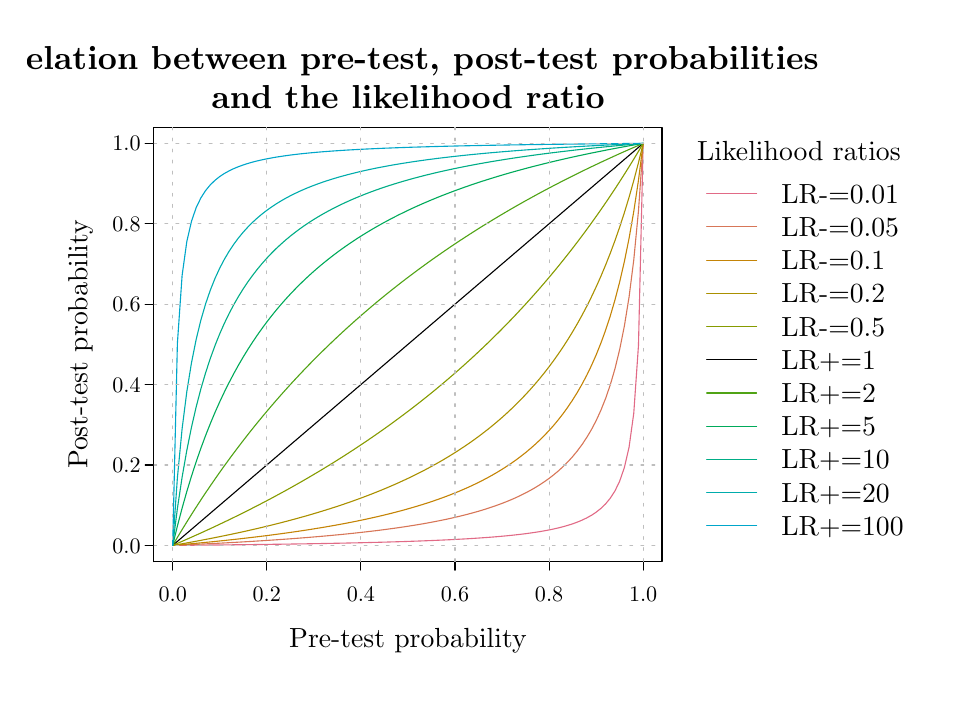
\begin{tikzpicture}[x=1pt,y=1pt]
\definecolor{fillColor}{RGB}{255,255,255}
\path[use as bounding box,fill=fillColor,fill opacity=0.00] (0,0) rectangle (325.21,238.49);
\begin{scope}
\path[clip] ( 45.60, 45.60) rectangle (229.21,202.49);
\definecolor{drawColor}{RGB}{0,0,0}

\path[draw=drawColor,line width= 0.4pt,line join=round,line cap=round] ( 52.40, 51.41) --
	( 54.10, 52.86) --
	( 55.80, 54.32) --
	( 57.50, 55.77) --
	( 59.20, 57.22) --
	( 60.90, 58.67) --
	( 62.60, 60.13) --
	( 64.30, 61.58) --
	( 66.00, 63.03) --
	( 67.70, 64.49) --
	( 69.40, 65.94) --
	( 71.10, 67.39) --
	( 72.80, 68.84) --
	( 74.50, 70.30) --
	( 76.20, 71.75) --
	( 77.90, 73.20) --
	( 79.60, 74.65) --
	( 81.30, 76.11) --
	( 83.00, 77.56) --
	( 84.70, 79.01) --
	( 86.40, 80.46) --
	( 88.10, 81.92) --
	( 89.80, 83.37) --
	( 91.50, 84.82) --
	( 93.20, 86.28) --
	( 94.90, 87.73) --
	( 96.60, 89.18) --
	( 98.30, 90.63) --
	(100.00, 92.09) --
	(101.70, 93.54) --
	(103.40, 94.99) --
	(105.10, 96.44) --
	(106.80, 97.90) --
	(108.51, 99.35) --
	(110.21,100.80) --
	(111.91,102.26) --
	(113.61,103.71) --
	(115.31,105.16) --
	(117.01,106.61) --
	(118.71,108.07) --
	(120.41,109.52) --
	(122.11,110.97) --
	(123.81,112.42) --
	(125.51,113.88) --
	(127.21,115.33) --
	(128.91,116.78) --
	(130.61,118.23) --
	(132.31,119.69) --
	(134.01,121.14) --
	(135.71,122.59) --
	(137.41,124.05) --
	(139.11,125.50) --
	(140.81,126.95) --
	(142.51,128.40) --
	(144.21,129.86) --
	(145.91,131.31) --
	(147.61,132.76) --
	(149.31,134.21) --
	(151.01,135.67) --
	(152.71,137.12) --
	(154.41,138.57) --
	(156.11,140.03) --
	(157.81,141.48) --
	(159.51,142.93) --
	(161.21,144.38) --
	(162.91,145.84) --
	(164.61,147.29) --
	(166.31,148.74) --
	(168.01,150.19) --
	(169.71,151.65) --
	(171.41,153.10) --
	(173.11,154.55) --
	(174.81,156.00) --
	(176.51,157.46) --
	(178.21,158.91) --
	(179.91,160.36) --
	(181.61,161.82) --
	(183.31,163.27) --
	(185.01,164.72) --
	(186.71,166.17) --
	(188.41,167.63) --
	(190.11,169.08) --
	(191.81,170.53) --
	(193.51,171.98) --
	(195.21,173.44) --
	(196.91,174.89) --
	(198.61,176.34) --
	(200.31,177.80) --
	(202.01,179.25) --
	(203.71,180.70) --
	(205.41,182.15) --
	(207.11,183.61) --
	(208.81,185.06) --
	(210.51,186.51) --
	(212.21,187.96) --
	(213.91,189.42) --
	(215.61,190.87) --
	(217.31,192.32) --
	(219.01,193.77) --
	(220.71,195.23) --
	(222.41,196.68);
\end{scope}
\begin{scope}
\path[clip] (  0.00,  0.00) rectangle (325.21,238.49);
\definecolor{drawColor}{RGB}{0,0,0}

\path[draw=drawColor,line width= 0.4pt,line join=round,line cap=round] ( 52.40, 45.60) -- (222.41, 45.60);

\path[draw=drawColor,line width= 0.4pt,line join=round,line cap=round] ( 52.40, 45.60) -- ( 52.40, 42.46);

\path[draw=drawColor,line width= 0.4pt,line join=round,line cap=round] ( 86.40, 45.60) -- ( 86.40, 42.46);

\path[draw=drawColor,line width= 0.4pt,line join=round,line cap=round] (120.41, 45.60) -- (120.41, 42.46);

\path[draw=drawColor,line width= 0.4pt,line join=round,line cap=round] (154.41, 45.60) -- (154.41, 42.46);

\path[draw=drawColor,line width= 0.4pt,line join=round,line cap=round] (188.41, 45.60) -- (188.41, 42.46);

\path[draw=drawColor,line width= 0.4pt,line join=round,line cap=round] (222.41, 45.60) -- (222.41, 42.46);

\node[text=drawColor,anchor=base,inner sep=0pt, outer sep=0pt, scale=  0.80] at ( 52.40, 31.20) {0.0};

\node[text=drawColor,anchor=base,inner sep=0pt, outer sep=0pt, scale=  0.80] at ( 86.40, 31.20) {0.2};

\node[text=drawColor,anchor=base,inner sep=0pt, outer sep=0pt, scale=  0.80] at (120.41, 31.20) {0.4};

\node[text=drawColor,anchor=base,inner sep=0pt, outer sep=0pt, scale=  0.80] at (154.41, 31.20) {0.6};

\node[text=drawColor,anchor=base,inner sep=0pt, outer sep=0pt, scale=  0.80] at (188.41, 31.20) {0.8};

\node[text=drawColor,anchor=base,inner sep=0pt, outer sep=0pt, scale=  0.80] at (222.41, 31.20) {1.0};

\path[draw=drawColor,line width= 0.4pt,line join=round,line cap=round] ( 45.60, 51.41) -- ( 45.60,196.68);

\path[draw=drawColor,line width= 0.4pt,line join=round,line cap=round] ( 45.60, 51.41) -- ( 42.46, 51.41);

\path[draw=drawColor,line width= 0.4pt,line join=round,line cap=round] ( 45.60, 80.46) -- ( 42.46, 80.46);

\path[draw=drawColor,line width= 0.4pt,line join=round,line cap=round] ( 45.60,109.52) -- ( 42.46,109.52);

\path[draw=drawColor,line width= 0.4pt,line join=round,line cap=round] ( 45.60,138.57) -- ( 42.46,138.57);

\path[draw=drawColor,line width= 0.4pt,line join=round,line cap=round] ( 45.60,167.63) -- ( 42.46,167.63);

\path[draw=drawColor,line width= 0.4pt,line join=round,line cap=round] ( 45.60,196.68) -- ( 42.46,196.68);

\node[text=drawColor,anchor=base east,inner sep=0pt, outer sep=0pt, scale=  0.80] at ( 40.80, 48.66) {0.0};

\node[text=drawColor,anchor=base east,inner sep=0pt, outer sep=0pt, scale=  0.80] at ( 40.80, 77.71) {0.2};

\node[text=drawColor,anchor=base east,inner sep=0pt, outer sep=0pt, scale=  0.80] at ( 40.80,106.76) {0.4};

\node[text=drawColor,anchor=base east,inner sep=0pt, outer sep=0pt, scale=  0.80] at ( 40.80,135.82) {0.6};

\node[text=drawColor,anchor=base east,inner sep=0pt, outer sep=0pt, scale=  0.80] at ( 40.80,164.87) {0.8};

\node[text=drawColor,anchor=base east,inner sep=0pt, outer sep=0pt, scale=  0.80] at ( 40.80,193.93) {1.0};

\path[draw=drawColor,line width= 0.4pt,line join=round,line cap=round] ( 45.60, 45.60) --
	(229.21, 45.60) --
	(229.21,202.49) --
	( 45.60,202.49) --
	( 45.60, 45.60);
\end{scope}
\begin{scope}
\path[clip] (  0.00,  0.00) rectangle (325.21,238.49);
\definecolor{drawColor}{RGB}{0,0,0}

\node[text=drawColor,anchor=base,inner sep=0pt, outer sep=0pt, scale=  1.20] at (137.41,223.55) {\bfseries Relation between pre-test, post-test probabilities};

\node[text=drawColor,anchor=base,inner sep=0pt, outer sep=0pt, scale=  1.20] at (137.41,209.15) {\bfseries  and the likelihood ratio};

\node[text=drawColor,anchor=base,inner sep=0pt, outer sep=0pt, scale=  1.00] at (137.41, 14.40) {Pre-test probability};

\node[text=drawColor,rotate= 90.00,anchor=base,inner sep=0pt, outer sep=0pt, scale=  1.00] at ( 21.60,124.05) {Post-test probability};
\end{scope}
\begin{scope}
\path[clip] ( 45.60, 45.60) rectangle (229.21,202.49);
\definecolor{drawColor}{RGB}{225,106,134}

\path[draw=drawColor,line width= 0.4pt,line join=round,line cap=round] ( 52.40, 51.41) --
	( 54.10, 51.43) --
	( 55.80, 51.44) --
	( 57.50, 51.46) --
	( 59.20, 51.47) --
	( 60.90, 51.49) --
	( 62.60, 51.50) --
	( 64.30, 51.52) --
	( 66.00, 51.54) --
	( 67.70, 51.55) --
	( 69.40, 51.57) --
	( 71.10, 51.59) --
	( 72.80, 51.61) --
	( 74.50, 51.63) --
	( 76.20, 51.65) --
	( 77.90, 51.67) --
	( 79.60, 51.69) --
	( 81.30, 51.71) --
	( 83.00, 51.73) --
	( 84.70, 51.75) --
	( 86.40, 51.77) --
	( 88.10, 51.80) --
	( 89.80, 51.82) --
	( 91.50, 51.84) --
	( 93.20, 51.87) --
	( 94.90, 51.89) --
	( 96.60, 51.92) --
	( 98.30, 51.95) --
	(100.00, 51.97) --
	(101.70, 52.00) --
	(103.40, 52.03) --
	(105.10, 52.06) --
	(106.80, 52.09) --
	(108.51, 52.12) --
	(110.21, 52.16) --
	(111.91, 52.19) --
	(113.61, 52.22) --
	(115.31, 52.26) --
	(117.01, 52.30) --
	(118.71, 52.33) --
	(120.41, 52.37) --
	(122.11, 52.41) --
	(123.81, 52.46) --
	(125.51, 52.50) --
	(127.21, 52.54) --
	(128.91, 52.59) --
	(130.61, 52.64) --
	(132.31, 52.69) --
	(134.01, 52.74) --
	(135.71, 52.79) --
	(137.41, 52.85) --
	(139.11, 52.91) --
	(140.81, 52.97) --
	(142.51, 53.03) --
	(144.21, 53.10) --
	(145.91, 53.16) --
	(147.61, 53.24) --
	(149.31, 53.31) --
	(151.01, 53.39) --
	(152.71, 53.47) --
	(154.41, 53.56) --
	(156.11, 53.65) --
	(157.81, 53.74) --
	(159.51, 53.84) --
	(161.21, 53.95) --
	(162.91, 54.06) --
	(164.61, 54.18) --
	(166.31, 54.30) --
	(168.01, 54.43) --
	(169.71, 54.57) --
	(171.41, 54.72) --
	(173.11, 54.88) --
	(174.81, 55.05) --
	(176.51, 55.24) --
	(178.21, 55.43) --
	(179.91, 55.64) --
	(181.61, 55.87) --
	(183.31, 56.12) --
	(185.01, 56.38) --
	(186.71, 56.68) --
	(188.41, 57.00) --
	(190.11, 57.35) --
	(191.81, 57.74) --
	(193.51, 58.17) --
	(195.21, 58.66) --
	(196.91, 59.20) --
	(198.61, 59.82) --
	(200.31, 60.52) --
	(202.01, 61.34) --
	(203.71, 62.28) --
	(205.41, 63.41) --
	(207.11, 64.75) --
	(208.81, 66.39) --
	(210.51, 68.45) --
	(212.21, 71.09) --
	(213.91, 74.61) --
	(215.61, 79.53) --
	(217.31, 86.90) --
	(219.01, 99.18) --
	(220.71,123.68) --
	(222.41,196.68);
\definecolor{drawColor}{RGB}{215,118,88}

\path[draw=drawColor,line width= 0.4pt,line join=round,line cap=round] ( 52.40, 51.41) --
	( 54.10, 51.48) --
	( 55.80, 51.56) --
	( 57.50, 51.64) --
	( 59.20, 51.71) --
	( 60.90, 51.79) --
	( 62.60, 51.87) --
	( 64.30, 51.96) --
	( 66.00, 52.04) --
	( 67.70, 52.13) --
	( 69.40, 52.21) --
	( 71.10, 52.30) --
	( 72.80, 52.39) --
	( 74.50, 52.49) --
	( 76.20, 52.58) --
	( 77.90, 52.68) --
	( 79.60, 52.78) --
	( 81.30, 52.88) --
	( 83.00, 52.99) --
	( 84.70, 53.09) --
	( 86.40, 53.20) --
	( 88.10, 53.32) --
	( 89.80, 53.43) --
	( 91.50, 53.55) --
	( 93.20, 53.67) --
	( 94.90, 53.79) --
	( 96.60, 53.92) --
	( 98.30, 54.05) --
	(100.00, 54.18) --
	(101.70, 54.32) --
	(103.40, 54.46) --
	(105.10, 54.60) --
	(106.80, 54.75) --
	(108.51, 54.90) --
	(110.21, 55.06) --
	(111.91, 55.22) --
	(113.61, 55.38) --
	(115.31, 55.55) --
	(117.01, 55.73) --
	(118.71, 55.91) --
	(120.41, 56.10) --
	(122.11, 56.29) --
	(123.81, 56.49) --
	(125.51, 56.69) --
	(127.21, 56.90) --
	(128.91, 57.12) --
	(130.61, 57.35) --
	(132.31, 57.58) --
	(134.01, 57.82) --
	(135.71, 58.07) --
	(137.41, 58.33) --
	(139.11, 58.60) --
	(140.81, 58.88) --
	(142.51, 59.16) --
	(144.21, 59.46) --
	(145.91, 59.78) --
	(147.61, 60.10) --
	(149.31, 60.44) --
	(151.01, 60.79) --
	(152.71, 61.16) --
	(154.41, 61.55) --
	(156.11, 61.95) --
	(157.81, 62.37) --
	(159.51, 62.81) --
	(161.21, 63.27) --
	(162.91, 63.75) --
	(164.61, 64.26) --
	(166.31, 64.80) --
	(168.01, 65.36) --
	(169.71, 65.96) --
	(171.41, 66.59) --
	(173.11, 67.25) --
	(174.81, 67.96) --
	(176.51, 68.71) --
	(178.21, 69.51) --
	(179.91, 70.36) --
	(181.61, 71.27) --
	(183.31, 72.24) --
	(185.01, 73.29) --
	(186.71, 74.41) --
	(188.41, 75.62) --
	(190.11, 76.94) --
	(191.81, 78.36) --
	(193.51, 79.92) --
	(195.21, 81.62) --
	(196.91, 83.48) --
	(198.61, 85.55) --
	(200.31, 87.83) --
	(202.01, 90.39) --
	(203.71, 93.25) --
	(205.41, 96.49) --
	(207.11,100.19) --
	(208.81,104.45) --
	(210.51,109.39) --
	(212.21,115.22) --
	(213.91,122.18) --
	(215.61,130.65) --
	(217.31,141.16) --
	(219.01,154.57) --
	(220.71,172.27) --
	(222.41,196.68);
\definecolor{drawColor}{RGB}{196,132,7}

\path[draw=drawColor,line width= 0.4pt,line join=round,line cap=round] ( 52.40, 51.41) --
	( 54.10, 51.56) --
	( 55.80, 51.71) --
	( 57.50, 51.86) --
	( 59.20, 52.01) --
	( 60.90, 52.17) --
	( 62.60, 52.33) --
	( 64.30, 52.50) --
	( 66.00, 52.66) --
	( 67.70, 52.83) --
	( 69.40, 53.01) --
	( 71.10, 53.18) --
	( 72.80, 53.37) --
	( 74.50, 53.55) --
	( 76.20, 53.74) --
	( 77.90, 53.93) --
	( 79.60, 54.13) --
	( 81.30, 54.33) --
	( 83.00, 54.53) --
	( 84.70, 54.74) --
	( 86.40, 54.95) --
	( 88.10, 55.17) --
	( 89.80, 55.40) --
	( 91.50, 55.62) --
	( 93.20, 55.86) --
	( 94.90, 56.10) --
	( 96.60, 56.34) --
	( 98.30, 56.59) --
	(100.00, 56.85) --
	(101.70, 57.11) --
	(103.40, 57.38) --
	(105.10, 57.66) --
	(106.80, 57.94) --
	(108.51, 58.23) --
	(110.21, 58.53) --
	(111.91, 58.83) --
	(113.61, 59.15) --
	(115.31, 59.47) --
	(117.01, 59.80) --
	(118.71, 60.14) --
	(120.41, 60.49) --
	(122.11, 60.85) --
	(123.81, 61.22) --
	(125.51, 61.60) --
	(127.21, 61.99) --
	(128.91, 62.40) --
	(130.61, 62.81) --
	(132.31, 63.24) --
	(134.01, 63.69) --
	(135.71, 64.14) --
	(137.41, 64.62) --
	(139.11, 65.11) --
	(140.81, 65.61) --
	(142.51, 66.13) --
	(144.21, 66.67) --
	(145.91, 67.23) --
	(147.61, 67.81) --
	(149.31, 68.41) --
	(151.01, 69.04) --
	(152.71, 69.69) --
	(154.41, 70.36) --
	(156.11, 71.06) --
	(157.81, 71.79) --
	(159.51, 72.55) --
	(161.21, 73.34) --
	(162.91, 74.16) --
	(164.61, 75.03) --
	(166.31, 75.93) --
	(168.01, 76.87) --
	(169.71, 77.86) --
	(171.41, 78.89) --
	(173.11, 79.98) --
	(174.81, 81.12) --
	(176.51, 82.33) --
	(178.21, 83.60) --
	(179.91, 84.93) --
	(181.61, 86.35) --
	(183.31, 87.85) --
	(185.01, 89.43) --
	(186.71, 91.12) --
	(188.41, 92.92) --
	(190.11, 94.83) --
	(191.81, 96.88) --
	(193.51, 99.07) --
	(195.21,101.42) --
	(196.91,103.96) --
	(198.61,106.69) --
	(200.31,109.65) --
	(202.01,112.87) --
	(203.71,116.38) --
	(205.41,120.22) --
	(207.11,124.45) --
	(208.81,129.11) --
	(210.51,134.29) --
	(212.21,140.08) --
	(213.91,146.59) --
	(215.61,153.95) --
	(217.31,162.36) --
	(219.01,172.06) --
	(220.71,183.35) --
	(222.41,196.68);
\definecolor{drawColor}{RGB}{170,144,0}

\path[draw=drawColor,line width= 0.4pt,line join=round,line cap=round] ( 52.40, 51.41) --
	( 54.10, 51.70) --
	( 55.80, 52.00) --
	( 57.50, 52.30) --
	( 59.20, 52.61) --
	( 60.90, 52.92) --
	( 62.60, 53.24) --
	( 64.30, 53.57) --
	( 66.00, 53.89) --
	( 67.70, 54.23) --
	( 69.40, 54.57) --
	( 71.10, 54.92) --
	( 72.80, 55.27) --
	( 74.50, 55.63) --
	( 76.20, 55.99) --
	( 77.90, 56.36) --
	( 79.60, 56.74) --
	( 81.30, 57.13) --
	( 83.00, 57.52) --
	( 84.70, 57.92) --
	( 86.40, 58.33) --
	( 88.10, 58.74) --
	( 89.80, 59.17) --
	( 91.50, 59.60) --
	( 93.20, 60.04) --
	( 94.90, 60.49) --
	( 96.60, 60.95) --
	( 98.30, 61.42) --
	(100.00, 61.89) --
	(101.70, 62.38) --
	(103.40, 62.88) --
	(105.10, 63.39) --
	(106.80, 63.91) --
	(108.51, 64.44) --
	(110.21, 64.98) --
	(111.91, 65.53) --
	(113.61, 66.10) --
	(115.31, 66.68) --
	(117.01, 67.27) --
	(118.71, 67.88) --
	(120.41, 68.50) --
	(122.11, 69.14) --
	(123.81, 69.79) --
	(125.51, 70.46) --
	(127.21, 71.14) --
	(128.91, 71.84) --
	(130.61, 72.56) --
	(132.31, 73.29) --
	(134.01, 74.05) --
	(135.71, 74.83) --
	(137.41, 75.62) --
	(139.11, 76.44) --
	(140.81, 77.28) --
	(142.51, 78.14) --
	(144.21, 79.03) --
	(145.91, 79.95) --
	(147.61, 80.89) --
	(149.31, 81.85) --
	(151.01, 82.85) --
	(152.71, 83.88) --
	(154.41, 84.93) --
	(156.11, 86.03) --
	(157.81, 87.15) --
	(159.51, 88.31) --
	(161.21, 89.51) --
	(162.91, 90.75) --
	(164.61, 92.04) --
	(166.31, 93.36) --
	(168.01, 94.74) --
	(169.71, 96.16) --
	(171.41, 97.63) --
	(173.11, 99.16) --
	(174.81,100.75) --
	(176.51,102.39) --
	(178.21,104.11) --
	(179.91,105.89) --
	(181.61,107.74) --
	(183.31,109.67) --
	(185.01,111.68) --
	(186.71,113.78) --
	(188.41,115.97) --
	(190.11,118.27) --
	(191.81,120.67) --
	(193.51,123.18) --
	(195.21,125.82) --
	(196.91,128.59) --
	(198.61,131.50) --
	(200.31,134.56) --
	(202.01,137.79) --
	(203.71,141.20) --
	(205.41,144.80) --
	(207.11,148.61) --
	(208.81,152.66) --
	(210.51,156.96) --
	(212.21,161.53) --
	(213.91,166.42) --
	(215.61,171.63) --
	(217.31,177.22) --
	(219.01,183.23) --
	(220.71,189.70) --
	(222.41,196.68);
\definecolor{drawColor}{RGB}{134,155,0}

\path[draw=drawColor,line width= 0.4pt,line join=round,line cap=round] ( 52.40, 51.41) --
	( 54.10, 52.14) --
	( 55.80, 52.88) --
	( 57.50, 53.62) --
	( 59.20, 54.38) --
	( 60.90, 55.14) --
	( 62.60, 55.90) --
	( 64.30, 56.68) --
	( 66.00, 57.46) --
	( 67.70, 58.26) --
	( 69.40, 59.06) --
	( 71.10, 59.87) --
	( 72.80, 60.68) --
	( 74.50, 61.51) --
	( 76.20, 62.35) --
	( 77.90, 63.19) --
	( 79.60, 64.04) --
	( 81.30, 64.91) --
	( 83.00, 65.78) --
	( 84.70, 66.66) --
	( 86.40, 67.55) --
	( 88.10, 68.45) --
	( 89.80, 69.37) --
	( 91.50, 70.29) --
	( 93.20, 71.22) --
	( 94.90, 72.16) --
	( 96.60, 73.12) --
	( 98.30, 74.08) --
	(100.00, 75.06) --
	(101.70, 76.05) --
	(103.40, 77.05) --
	(105.10, 78.06) --
	(106.80, 79.08) --
	(108.51, 80.12) --
	(110.21, 81.16) --
	(111.91, 82.23) --
	(113.61, 83.30) --
	(115.31, 84.39) --
	(117.01, 85.49) --
	(118.71, 86.60) --
	(120.41, 87.73) --
	(122.11, 88.87) --
	(123.81, 90.03) --
	(125.51, 91.20) --
	(127.21, 92.38) --
	(128.91, 93.59) --
	(130.61, 94.80) --
	(132.31, 96.04) --
	(134.01, 97.29) --
	(135.71, 98.55) --
	(137.41, 99.83) --
	(139.11,101.13) --
	(140.81,102.45) --
	(142.51,103.79) --
	(144.21,105.14) --
	(145.91,106.51) --
	(147.61,107.90) --
	(149.31,109.32) --
	(151.01,110.75) --
	(152.71,112.20) --
	(154.41,113.67) --
	(156.11,115.16) --
	(157.81,116.68) --
	(159.51,118.21) --
	(161.21,119.77) --
	(162.91,121.36) --
	(164.61,122.96) --
	(166.31,124.59) --
	(168.01,126.25) --
	(169.71,127.93) --
	(171.41,129.63) --
	(173.11,131.37) --
	(174.81,133.12) --
	(176.51,134.91) --
	(178.21,136.73) --
	(179.91,138.57) --
	(181.61,140.45) --
	(183.31,142.35) --
	(185.01,144.29) --
	(186.71,146.26) --
	(188.41,148.26) --
	(190.11,150.29) --
	(191.81,152.36) --
	(193.51,154.47) --
	(195.21,156.61) --
	(196.91,158.78) --
	(198.61,161.00) --
	(200.31,163.26) --
	(202.01,165.55) --
	(203.71,167.89) --
	(205.41,170.27) --
	(207.11,172.69) --
	(208.81,175.16) --
	(210.51,177.67) --
	(212.21,180.23) --
	(213.91,182.85) --
	(215.61,185.51) --
	(217.31,188.22) --
	(219.01,190.98) --
	(220.71,193.80) --
	(222.41,196.68);
\definecolor{drawColor}{RGB}{80,163,21}

\path[draw=drawColor,line width= 0.4pt,line join=round,line cap=round] ( 52.40, 51.41) --
	( 54.10, 54.29) --
	( 55.80, 57.11) --
	( 57.50, 59.87) --
	( 59.20, 62.59) --
	( 60.90, 65.25) --
	( 62.60, 67.86) --
	( 64.30, 70.42) --
	( 66.00, 72.93) --
	( 67.70, 75.40) --
	( 69.40, 77.82) --
	( 71.10, 80.20) --
	( 72.80, 82.54) --
	( 74.50, 84.84) --
	( 76.20, 87.09) --
	( 77.90, 89.31) --
	( 79.60, 91.49) --
	( 81.30, 93.63) --
	( 83.00, 95.73) --
	( 84.70, 97.80) --
	( 86.40, 99.83) --
	( 88.10,101.83) --
	( 89.80,103.80) --
	( 91.50,105.74) --
	( 93.20,107.64) --
	( 94.90,109.52) --
	( 96.60,111.36) --
	( 98.30,113.18) --
	(100.00,114.97) --
	(101.70,116.73) --
	(103.40,118.46) --
	(105.10,120.16) --
	(106.80,121.84) --
	(108.51,123.50) --
	(110.21,125.13) --
	(111.91,126.74) --
	(113.61,128.32) --
	(115.31,129.88) --
	(117.01,131.41) --
	(118.71,132.93) --
	(120.41,134.42) --
	(122.11,135.89) --
	(123.81,137.34) --
	(125.51,138.78) --
	(127.21,140.19) --
	(128.91,141.58) --
	(130.61,142.95) --
	(132.31,144.30) --
	(134.01,145.64) --
	(135.71,146.96) --
	(137.41,148.26) --
	(139.11,149.54) --
	(140.81,150.81) --
	(142.51,152.05) --
	(144.21,153.29) --
	(145.91,154.51) --
	(147.61,155.71) --
	(149.31,156.89) --
	(151.01,158.06) --
	(152.71,159.22) --
	(154.41,160.36) --
	(156.11,161.49) --
	(157.81,162.60) --
	(159.51,163.70) --
	(161.21,164.79) --
	(162.91,165.87) --
	(164.61,166.93) --
	(166.31,167.97) --
	(168.01,169.01) --
	(169.71,170.03) --
	(171.41,171.04) --
	(173.11,172.04) --
	(174.81,173.03) --
	(176.51,174.01) --
	(178.21,174.97) --
	(179.91,175.93) --
	(181.61,176.87) --
	(183.31,177.80) --
	(185.01,178.73) --
	(186.71,179.64) --
	(188.41,180.54) --
	(190.11,181.43) --
	(191.81,182.31) --
	(193.51,183.19) --
	(195.21,184.05) --
	(196.91,184.90) --
	(198.61,185.75) --
	(200.31,186.58) --
	(202.01,187.41) --
	(203.71,188.23) --
	(205.41,189.03) --
	(207.11,189.84) --
	(208.81,190.63) --
	(210.51,191.41) --
	(212.21,192.19) --
	(213.91,192.96) --
	(215.61,193.72) --
	(217.31,194.47) --
	(219.01,195.21) --
	(220.71,195.95) --
	(222.41,196.68);
\definecolor{drawColor}{RGB}{0,170,90}

\path[draw=drawColor,line width= 0.4pt,line join=round,line cap=round] ( 52.40, 51.41) --
	( 54.10, 58.39) --
	( 55.80, 64.86) --
	( 57.50, 70.87) --
	( 59.20, 76.46) --
	( 60.90, 81.68) --
	( 62.60, 86.56) --
	( 64.30, 91.13) --
	( 66.00, 95.43) --
	( 67.70, 99.48) --
	( 69.40,103.29) --
	( 71.10,106.90) --
	( 72.80,110.30) --
	( 74.50,113.53) --
	( 76.20,116.60) --
	( 77.90,119.51) --
	( 79.60,122.27) --
	( 81.30,124.91) --
	( 83.00,127.42) --
	( 84.70,129.82) --
	( 86.40,132.12) --
	( 88.10,134.31) --
	( 89.80,136.41) --
	( 91.50,138.42) --
	( 93.20,140.35) --
	( 94.90,142.20) --
	( 96.60,143.98) --
	( 98.30,145.70) --
	(100.00,147.34) --
	(101.70,148.93) --
	(103.40,150.46) --
	(105.10,151.93) --
	(106.80,153.35) --
	(108.51,154.73) --
	(110.21,156.05) --
	(111.91,157.34) --
	(113.61,158.58) --
	(115.31,159.78) --
	(117.01,160.94) --
	(118.71,162.07) --
	(120.41,163.16) --
	(122.11,164.21) --
	(123.81,165.24) --
	(125.51,166.24) --
	(127.21,167.21) --
	(128.91,168.15) --
	(130.61,169.06) --
	(132.31,169.95) --
	(134.01,170.81) --
	(135.71,171.65) --
	(137.41,172.47) --
	(139.11,173.27) --
	(140.81,174.04) --
	(142.51,174.80) --
	(144.21,175.53) --
	(145.91,176.25) --
	(147.61,176.95) --
	(149.31,177.64) --
	(151.01,178.30) --
	(152.71,178.95) --
	(154.41,179.59) --
	(156.11,180.21) --
	(157.81,180.82) --
	(159.51,181.41) --
	(161.21,181.99) --
	(162.91,182.56) --
	(164.61,183.11) --
	(166.31,183.65) --
	(168.01,184.18) --
	(169.71,184.70) --
	(171.41,185.21) --
	(173.11,185.71) --
	(174.81,186.20) --
	(176.51,186.67) --
	(178.21,187.14) --
	(179.91,187.60) --
	(181.61,188.05) --
	(183.31,188.49) --
	(185.01,188.92) --
	(186.71,189.35) --
	(188.41,189.76) --
	(190.11,190.17) --
	(191.81,190.57) --
	(193.51,190.96) --
	(195.21,191.35) --
	(196.91,191.73) --
	(198.61,192.10) --
	(200.31,192.46) --
	(202.01,192.82) --
	(203.71,193.18) --
	(205.41,193.52) --
	(207.11,193.86) --
	(208.81,194.20) --
	(210.51,194.53) --
	(212.21,194.85) --
	(213.91,195.17) --
	(215.61,195.48) --
	(217.31,195.79) --
	(219.01,196.09) --
	(220.71,196.39) --
	(222.41,196.68);
\definecolor{drawColor}{RGB}{0,173,134}

\path[draw=drawColor,line width= 0.4pt,line join=round,line cap=round] ( 52.40, 51.41) --
	( 54.10, 64.74) --
	( 55.80, 76.03) --
	( 57.50, 85.73) --
	( 59.20, 94.14) --
	( 60.90,101.50) --
	( 62.60,108.01) --
	( 64.30,113.80) --
	( 66.00,118.98) --
	( 67.70,123.64) --
	( 69.40,127.87) --
	( 71.10,131.71) --
	( 72.80,135.22) --
	( 74.50,138.44) --
	( 76.20,141.40) --
	( 77.90,144.14) --
	( 79.60,146.67) --
	( 81.30,149.02) --
	( 83.00,151.21) --
	( 84.70,153.26) --
	( 86.40,155.17) --
	( 88.10,156.97) --
	( 89.80,158.66) --
	( 91.50,160.24) --
	( 93.20,161.74) --
	( 94.90,163.16) --
	( 96.60,164.49) --
	( 98.30,165.76) --
	(100.00,166.97) --
	(101.70,168.11) --
	(103.40,169.20) --
	(105.10,170.23) --
	(106.80,171.22) --
	(108.51,172.16) --
	(110.21,173.06) --
	(111.91,173.93) --
	(113.61,174.75) --
	(115.31,175.54) --
	(117.01,176.30) --
	(118.71,177.03) --
	(120.41,177.73) --
	(122.11,178.41) --
	(123.81,179.05) --
	(125.51,179.68) --
	(127.21,180.28) --
	(128.91,180.86) --
	(130.61,181.42) --
	(132.31,181.96) --
	(134.01,182.48) --
	(135.71,182.99) --
	(137.41,183.47) --
	(139.11,183.95) --
	(140.81,184.40) --
	(142.51,184.85) --
	(144.21,185.28) --
	(145.91,185.69) --
	(147.61,186.10) --
	(149.31,186.49) --
	(151.01,186.87) --
	(152.71,187.24) --
	(154.41,187.60) --
	(156.11,187.95) --
	(157.81,188.29) --
	(159.51,188.62) --
	(161.21,188.94) --
	(162.91,189.26) --
	(164.61,189.56) --
	(166.31,189.86) --
	(168.01,190.15) --
	(169.71,190.43) --
	(171.41,190.71) --
	(173.11,190.98) --
	(174.81,191.24) --
	(176.51,191.50) --
	(178.21,191.75) --
	(179.91,191.99) --
	(181.61,192.23) --
	(183.31,192.47) --
	(185.01,192.70) --
	(186.71,192.92) --
	(188.41,193.14) --
	(190.11,193.35) --
	(191.81,193.56) --
	(193.51,193.76) --
	(195.21,193.96) --
	(196.91,194.16) --
	(198.61,194.35) --
	(200.31,194.54) --
	(202.01,194.73) --
	(203.71,194.91) --
	(205.41,195.08) --
	(207.11,195.26) --
	(208.81,195.43) --
	(210.51,195.59) --
	(212.21,195.76) --
	(213.91,195.92) --
	(215.61,196.08) --
	(217.31,196.23) --
	(219.01,196.38) --
	(220.71,196.53) --
	(222.41,196.68);
\definecolor{drawColor}{RGB}{0,172,172}

\path[draw=drawColor,line width= 0.4pt,line join=round,line cap=round] ( 52.40, 51.41) --
	( 54.10, 75.83) --
	( 55.80, 93.52) --
	( 57.50,106.93) --
	( 59.20,117.44) --
	( 60.90,125.91) --
	( 62.60,132.87) --
	( 64.30,138.70) --
	( 66.00,143.65) --
	( 67.70,147.90) --
	( 69.40,151.60) --
	( 71.10,154.84) --
	( 72.80,157.71) --
	( 74.50,160.26) --
	( 76.20,162.55) --
	( 77.90,164.61) --
	( 79.60,166.48) --
	( 81.30,168.18) --
	( 83.00,169.73) --
	( 84.70,171.16) --
	( 86.40,172.47) --
	( 88.10,173.68) --
	( 89.80,174.81) --
	( 91.50,175.85) --
	( 93.20,176.82) --
	( 94.90,177.73) --
	( 96.60,178.58) --
	( 98.30,179.38) --
	(100.00,180.13) --
	(101.70,180.84) --
	(103.40,181.50) --
	(105.10,182.13) --
	(106.80,182.73) --
	(108.51,183.29) --
	(110.21,183.83) --
	(111.91,184.34) --
	(113.61,184.82) --
	(115.31,185.28) --
	(117.01,185.72) --
	(118.71,186.14) --
	(120.41,186.55) --
	(122.11,186.93) --
	(123.81,187.30) --
	(125.51,187.65) --
	(127.21,187.99) --
	(128.91,188.31) --
	(130.61,188.63) --
	(132.31,188.93) --
	(134.01,189.22) --
	(135.71,189.49) --
	(137.41,189.76) --
	(139.11,190.02) --
	(140.81,190.27) --
	(142.51,190.51) --
	(144.21,190.75) --
	(145.91,190.97) --
	(147.61,191.19) --
	(149.31,191.40) --
	(151.01,191.60) --
	(152.71,191.80) --
	(154.41,191.99) --
	(156.11,192.18) --
	(157.81,192.36) --
	(159.51,192.54) --
	(161.21,192.71) --
	(162.91,192.87) --
	(164.61,193.03) --
	(166.31,193.19) --
	(168.01,193.34) --
	(169.71,193.49) --
	(171.41,193.63) --
	(173.11,193.77) --
	(174.81,193.91) --
	(176.51,194.04) --
	(178.21,194.17) --
	(179.91,194.30) --
	(181.61,194.42) --
	(183.31,194.54) --
	(185.01,194.66) --
	(186.71,194.77) --
	(188.41,194.89) --
	(190.11,195.00) --
	(191.81,195.10) --
	(193.51,195.21) --
	(195.21,195.31) --
	(196.91,195.41) --
	(198.61,195.51) --
	(200.31,195.60) --
	(202.01,195.70) --
	(203.71,195.79) --
	(205.41,195.88) --
	(207.11,195.97) --
	(208.81,196.05) --
	(210.51,196.14) --
	(212.21,196.22) --
	(213.91,196.30) --
	(215.61,196.38) --
	(217.31,196.46) --
	(219.01,196.53) --
	(220.71,196.61) --
	(222.41,196.68);
\definecolor{drawColor}{RGB}{0,166,202}

\path[draw=drawColor,line width= 0.4pt,line join=round,line cap=round] ( 52.40, 51.41) --
	( 54.10,124.41) --
	( 55.80,148.91) --
	( 57.50,161.19) --
	( 59.20,168.56) --
	( 60.90,173.49) --
	( 62.60,177.00) --
	( 64.30,179.64) --
	( 66.00,181.70) --
	( 67.70,183.34) --
	( 69.40,184.69) --
	( 71.10,185.81) --
	( 72.80,186.75) --
	( 74.50,187.57) --
	( 76.20,188.27) --
	( 77.90,188.89) --
	( 79.60,189.43) --
	( 81.30,189.92) --
	( 83.00,190.35) --
	( 84.70,190.74) --
	( 86.40,191.09) --
	( 88.10,191.41) --
	( 89.80,191.71) --
	( 91.50,191.97) --
	( 93.20,192.22) --
	( 94.90,192.45) --
	( 96.60,192.66) --
	( 98.30,192.86) --
	(100.00,193.04) --
	(101.70,193.21) --
	(103.40,193.37) --
	(105.10,193.52) --
	(106.80,193.66) --
	(108.51,193.79) --
	(110.21,193.91) --
	(111.91,194.03) --
	(113.61,194.14) --
	(115.31,194.25) --
	(117.01,194.35) --
	(118.71,194.44) --
	(120.41,194.53) --
	(122.11,194.62) --
	(123.81,194.70) --
	(125.51,194.78) --
	(127.21,194.85) --
	(128.91,194.93) --
	(130.61,194.99) --
	(132.31,195.06) --
	(134.01,195.12) --
	(135.71,195.18) --
	(137.41,195.24) --
	(139.11,195.30) --
	(140.81,195.35) --
	(142.51,195.40) --
	(144.21,195.45) --
	(145.91,195.50) --
	(147.61,195.55) --
	(149.31,195.59) --
	(151.01,195.64) --
	(152.71,195.68) --
	(154.41,195.72) --
	(156.11,195.76) --
	(157.81,195.80) --
	(159.51,195.83) --
	(161.21,195.87) --
	(162.91,195.90) --
	(164.61,195.94) --
	(166.31,195.97) --
	(168.01,196.00) --
	(169.71,196.03) --
	(171.41,196.06) --
	(173.11,196.09) --
	(174.81,196.12) --
	(176.51,196.14) --
	(178.21,196.17) --
	(179.91,196.20) --
	(181.61,196.22) --
	(183.31,196.25) --
	(185.01,196.27) --
	(186.71,196.30) --
	(188.41,196.32) --
	(190.11,196.34) --
	(191.81,196.36) --
	(193.51,196.38) --
	(195.21,196.40) --
	(196.91,196.42) --
	(198.61,196.44) --
	(200.31,196.46) --
	(202.01,196.48) --
	(203.71,196.50) --
	(205.41,196.52) --
	(207.11,196.54) --
	(208.81,196.55) --
	(210.51,196.57) --
	(212.21,196.59) --
	(213.91,196.60) --
	(215.61,196.62) --
	(217.31,196.64) --
	(219.01,196.65) --
	(220.71,196.67) --
	(222.41,196.68);
\definecolor{drawColor}{RGB}{190,190,190}

\path[draw=drawColor,line width= 0.4pt,dash pattern=on 1pt off 3pt ,line join=round,line cap=round] ( 45.60, 51.41) -- (229.21, 51.41);

\path[draw=drawColor,line width= 0.4pt,dash pattern=on 1pt off 3pt ,line join=round,line cap=round] ( 45.60, 80.46) -- (229.21, 80.46);

\path[draw=drawColor,line width= 0.4pt,dash pattern=on 1pt off 3pt ,line join=round,line cap=round] ( 45.60,109.52) -- (229.21,109.52);

\path[draw=drawColor,line width= 0.4pt,dash pattern=on 1pt off 3pt ,line join=round,line cap=round] ( 45.60,138.57) -- (229.21,138.57);

\path[draw=drawColor,line width= 0.4pt,dash pattern=on 1pt off 3pt ,line join=round,line cap=round] ( 45.60,167.63) -- (229.21,167.63);

\path[draw=drawColor,line width= 0.4pt,dash pattern=on 1pt off 3pt ,line join=round,line cap=round] ( 45.60,196.68) -- (229.21,196.68);

\path[draw=drawColor,line width= 0.4pt,dash pattern=on 1pt off 3pt ,line join=round,line cap=round] ( 52.40, 45.60) -- ( 52.40,202.49);

\path[draw=drawColor,line width= 0.4pt,dash pattern=on 1pt off 3pt ,line join=round,line cap=round] ( 86.40, 45.60) -- ( 86.40,202.49);

\path[draw=drawColor,line width= 0.4pt,dash pattern=on 1pt off 3pt ,line join=round,line cap=round] (120.41, 45.60) -- (120.41,202.49);

\path[draw=drawColor,line width= 0.4pt,dash pattern=on 1pt off 3pt ,line join=round,line cap=round] (154.41, 45.60) -- (154.41,202.49);

\path[draw=drawColor,line width= 0.4pt,dash pattern=on 1pt off 3pt ,line join=round,line cap=round] (188.41, 45.60) -- (188.41,202.49);

\path[draw=drawColor,line width= 0.4pt,dash pattern=on 1pt off 3pt ,line join=round,line cap=round] (222.41, 45.60) -- (222.41,202.49);
\end{scope}
\begin{scope}
\path[clip] (  0.00,  0.00) rectangle (325.21,238.49);
\definecolor{drawColor}{RGB}{225,106,134}

\path[draw=drawColor,line width= 0.4pt,line join=round,line cap=round] (245.37,178.49) -- (263.37,178.49);
\definecolor{drawColor}{RGB}{215,118,88}

\path[draw=drawColor,line width= 0.4pt,line join=round,line cap=round] (245.37,166.49) -- (263.37,166.49);
\definecolor{drawColor}{RGB}{196,132,7}

\path[draw=drawColor,line width= 0.4pt,line join=round,line cap=round] (245.37,154.49) -- (263.37,154.49);
\definecolor{drawColor}{RGB}{170,144,0}

\path[draw=drawColor,line width= 0.4pt,line join=round,line cap=round] (245.37,142.49) -- (263.37,142.49);
\definecolor{drawColor}{RGB}{134,155,0}

\path[draw=drawColor,line width= 0.4pt,line join=round,line cap=round] (245.37,130.49) -- (263.37,130.49);
\definecolor{drawColor}{RGB}{0,0,0}

\path[draw=drawColor,line width= 0.4pt,line join=round,line cap=round] (245.37,118.49) -- (263.37,118.49);
\definecolor{drawColor}{RGB}{80,163,21}

\path[draw=drawColor,line width= 0.4pt,line join=round,line cap=round] (245.37,106.49) -- (263.37,106.49);
\definecolor{drawColor}{RGB}{0,170,90}

\path[draw=drawColor,line width= 0.4pt,line join=round,line cap=round] (245.37, 94.49) -- (263.37, 94.49);
\definecolor{drawColor}{RGB}{0,173,134}

\path[draw=drawColor,line width= 0.4pt,line join=round,line cap=round] (245.37, 82.49) -- (263.37, 82.49);
\definecolor{drawColor}{RGB}{0,172,172}

\path[draw=drawColor,line width= 0.4pt,line join=round,line cap=round] (245.37, 70.49) -- (263.37, 70.49);
\definecolor{drawColor}{RGB}{0,166,202}

\path[draw=drawColor,line width= 0.4pt,line join=round,line cap=round] (245.37, 58.49) -- (263.37, 58.49);
\definecolor{drawColor}{RGB}{0,0,0}

\node[text=drawColor,anchor=base,inner sep=0pt, outer sep=0pt, scale=  1.00] at (278.69,190.49) {Likelihood ratios};

\node[text=drawColor,anchor=base west,inner sep=0pt, outer sep=0pt, scale=  1.00] at (272.37,175.05) {LR-=0.01};

\node[text=drawColor,anchor=base west,inner sep=0pt, outer sep=0pt, scale=  1.00] at (272.37,163.05) {LR-=0.05};

\node[text=drawColor,anchor=base west,inner sep=0pt, outer sep=0pt, scale=  1.00] at (272.37,151.05) {LR-=0.1};

\node[text=drawColor,anchor=base west,inner sep=0pt, outer sep=0pt, scale=  1.00] at (272.37,139.05) {LR-=0.2};

\node[text=drawColor,anchor=base west,inner sep=0pt, outer sep=0pt, scale=  1.00] at (272.37,127.05) {LR-=0.5};

\node[text=drawColor,anchor=base west,inner sep=0pt, outer sep=0pt, scale=  1.00] at (272.37,115.05) {LR+=1};

\node[text=drawColor,anchor=base west,inner sep=0pt, outer sep=0pt, scale=  1.00] at (272.37,103.05) {LR+=2};

\node[text=drawColor,anchor=base west,inner sep=0pt, outer sep=0pt, scale=  1.00] at (272.37, 91.05) {LR+=5};

\node[text=drawColor,anchor=base west,inner sep=0pt, outer sep=0pt, scale=  1.00] at (272.37, 79.05) {LR+=10};

\node[text=drawColor,anchor=base west,inner sep=0pt, outer sep=0pt, scale=  1.00] at (272.37, 67.05) {LR+=20};

\node[text=drawColor,anchor=base west,inner sep=0pt, outer sep=0pt, scale=  1.00] at (272.37, 55.05) {LR+=100};
\end{scope}
\end{tikzpicture}
}}
\end{center}
\end{frame}
